\documentclass[12pt]{report}
% had to change latex compiler to XeLatex to get this to work- used to be pdfLatex
\usepackage[utf8]{inputenc}
\usepackage{setspace}
%\usepackage{subfigure}

\pagestyle{plain}
\usepackage{amssymb,graphicx,color}
\usepackage{amsfonts}
\usepackage{float}
\usepackage{latexsym}
\usepackage{a4wide}
\usepackage{amsmath}
\usepackage{booktabs}
\usepackage{tabulary}
\usepackage{multirow}
\usepackage{bbm}
\usepackage{mathrsfs}

% very basic, number only
%\usepackage{biblatex}
%\addbibresource{refs.bib}


% Goldstone and Rogosky 2002
%\usepackage[backend=biber,
%style=numeric,
%citestyle=authoryear]{biblatex} 
%\addbibresource{refs.bib}

% [GR02]
\usepackage[backend=biber,
style=alphabetic,
citestyle=alphabetic]{biblatex} 
\addbibresource{refs.bib}


\usepackage{todonotes}

\newtheorem{theorem}{THEOREM}
\newtheorem{lemma}[theorem]{LEMMA}
\newtheorem{corollary}[theorem]{COROLLARY}
\newtheorem{proposition}[theorem]{PROPOSITION}
\newtheorem{remark}[theorem]{REMARK}
\newtheorem{definition}[theorem]{DEFINITION}
\newtheorem{fact}[theorem]{FACT}

\newtheorem{problem}[theorem]{PROBLEM}
\newtheorem{exercise}[theorem]{EXERCISE}
\def \set#1{\{#1\} }

\newenvironment{proof}{
PROOF:
\begin{quotation}}{
$\Box$ \end{quotation}}

\newcommand{\N}{\mathcal{N}}

\newcommand{\nats}{\mbox{\( \mathbb N \)}}
\newcommand{\rat}{\mbox{\(\mathbb Q\)}}
\newcommand{\rats}{\mbox{\(\mathbb Q\)}}
\newcommand{\reals}{\mbox{\(\mathbb R\)}}
\newcommand{\ints}{\mbox{\(\mathbb Z\)}}

\newcommand{\ddx}{\frac{d}{dx}}
\newcommand{\dfdx}{\frac{df}{dx}}
\newcommand{\ddxp}[1]{\frac{d}{dx}\left( #1 \right)}
\newcommand{\dydx}{\frac{dy}{dx}}
\newcommand{\ddtheta}{\frac{d}{d\theta}}
\newcommand{\ddalpha}{\frac{d}{d\alpha}}
\newcommand{\ddvectheta}{\frac{\partial}{\partial \vectheta}}
\newcommand{\veca}{\boldsymbol{a}}
\newcommand{\vece}{\boldsymbol{e}}
\newcommand{\vecx}{\boldsymbol{x}}
\newcommand{\vecphi}{\boldsymbol{\phi}}
\newcommand{\vecp}{\boldsymbol{p}}
\newcommand{\vecd}{\boldsymbol{d}}
\newcommand{\vecw}{\boldsymbol{w}}
\newcommand{\vecy}{\boldsymbol{y}}
\newcommand{\vecz}{\boldsymbol{z}}
\newcommand{\vecA}{\boldsymbol{A}}
\newcommand{\vecB}{\boldsymbol{B}}
\newcommand{\vecC}{\boldsymbol{C}}
\newcommand{\vecH}{\boldsymbol{H}}
\newcommand{\vecP}{\boldsymbol{P}}
\newcommand{\vecQ}{\boldsymbol{Q}}
\newcommand{\vecI}{\boldsymbol{I}}
\newcommand{\yhat}{\hat{y}}
\newcommand{\one}{\mathbbm{1}}
\newcommand{\bigO}{\boldsymbol{O}}
\newcommand{\vecLam}{\boldsymbol{\Lambda}}
\newcommand{\vecK}{\boldsymbol{K}}
\newcommand{\vecL}{\boldsymbol{L}}
\newcommand{\Lag}{\mathscr{L}}
\newcommand{\dlda}{\frac{\partial \Lag}{\partial \alpha}}
\newcommand{\dldb}{\frac{\partial \Lag}{\partial \beta}}
\newcommand{\Kt}{\tilde{K}}
\newcommand{\Lt}{\tilde{L}}
\newcommand{\vecX}{\boldsymbol{X}}
\newcommand{\vecY}{\boldsymbol{Y}}
\newcommand{\vecW}{\boldsymbol{W}}
\newcommand{\vecV}{\boldsymbol{V}}
\newcommand{\vecU}{\boldsymbol{U}}
\newcommand{\vecSigma}{\boldsymbol{\Sigma}}
\newcommand{\vecR}{\boldsymbol{R}}
\newcommand{\veczero}{\boldsymbol{0}}
\newcommand{\vecalpha}{\boldsymbol{\alpha}}
\newcommand{\vecbeta}{\boldsymbol{\beta}}
\newcommand{\ip}[1]{\langle#1\rangle}
\newcommand{\Biggip}[1]{\Bigg\langle#1\Bigg\rangle}
\newcommand{\xTx}{\ip{\vecx}{\vecx}}
\newcommand{\zTz}{\ip{\vecz}{\vecz}}
\newcommand{\xTAx}{\ip{\vecx}{\A\vecx}}
\newcommand{\fracn}{\frac{1}{n}}
\newcommand{\intx}[1]{\int #1 \, dx}
\newcommand{\intt}[1]{\int #1 \, dt}
\newcommand{\defint}[3]{\int_{#1}^{#2} #3 \, dx}
\newcommand{\imp}{\Rightarrow}
\newcommand{\un}{\cup}
\newcommand{\inter}{\cap}
\newcommand{\ps}{\mathscr{P}}
\newcommand{\ift}{~\text{if}~}
\newcommand{\owt}{~\text{otherwise}~}
\newcommand{\spaced}[1]{\quad \text{#1} \quad}
\newcommand{\argmax}[1]{\underset{#1}{\operatorname{argmax}}}
\newcommand{\argmin}[1]{\underset{#1}{\operatorname{argmin}}}
\newcommand{\Cxy}{\hat{C}_{XY}}
\newcommand{\Cxx}{\hat{C}_{XX}}
\newcommand{\Cyy}{\hat{C}_{YY}}
\newcommand{\Err}{\mathcal{E}}
\newcommand{\Alg}{\mathcal{A}}
\newcommand{\Seq}{\mathcal{S}}
\newcommand{\C}{\mathcal{C}}
\newcommand{\hs}{\mathcal{H}}
\newcommand{\I}{\mathcal{I}}
\newcommand{\R}{\mathbb{R}}
\newcommand{\onen}{\frac{1}{n}}
\newcommand{\sumin}{\sum_{i=1}^n}
\newcommand{\sumjn}{\sum_{j=1}^n}
\newcommand{\sumim}{\sum_{i=1}^m}
\newcommand{\sumjm}{\sum_{j=1}^m}
%%%%%%%%%%%%%%%%%%%%%%%%%%
\begin{document}

\title{  	{ 
\includegraphics[scale=.5]{ucl_logo.png}}\\
{{\Huge Semi-supervised Learning Of Jointly Aligned Concept Embeddings}}\\
%{\large There Is No Optional Subtitle Yet}\\
		}
\date{Submission date: Day Month Year}
\author{Petra Chong\thanks{
{\bf Disclaimer:}
This report is submitted as part requirement for the MSc in Machine Learning at UCL. It is
substantially the result of my own work except where explicitly indicated in the text.
The report may be freely copied and distributed provided the source is explicitly acknowledged.
}
\\ \\
MSc Machine Learning\\ \\
Professor Bradley Love}

 
\onehalfspacing
\maketitle
\begin{abstract}
We are interested in the problem of learning statistical representations of concepts from multimodal data, as this mimics the way that humans learn. Choosing to represent concepts as continuous vector embeddings, we use the GloVe algorithm to learn probabilistic embeddings from co-occurrence statistics of concepts in the Open Images and AudioSet datasets. We begin by learning embeddings for each modality independently, as a baseline, then we investigate an algorithm for jointly aligning probabilistic GloVe embeddings with no post-processing. We examine the use of the Maximum Mean Discrepancy distributional similarity measure to improve alignment. We analyse the quality of the resulting embeddings by comparison with three human-curated datasets, and we find that alignment increases embedding quality when compared to the largest of these datasets. This supports the findings of other studies in multi-task learning, which conclude that learning from multiple input streams results in models that generalise better. 
\end{abstract}

%
\newpage
\section*{Acknowledgements}

Special thanks are due to the following:

\begin{itemize}
    \item Professor Bradley Love, for the opportunity to work with the Love Lab.
    \item Dr. Brett Roads, for much help and guidance and access to \texttt{love17} and lots of computing power. 
    \item Professor Justine Cassell, for the opportunity to work in the Media Lab for my first dissertation, without which writing this one would have been much harder. 
    \item Dr. Chong Siew Meng (1950-2019) without whose influence I would not be such a massive geek. 
\end{itemize}
\tableofcontents
\setcounter{page}{1}

%\chapter{Known loose ends}


\begin{itemize}
    \item \todo[inline]{Incomplete literature review}
    \item \todo[inline]{Lots of equations missing}
    \item \todo[inline]{No diagrams}
    \item \todo[inline]{Lots of things still in point form}
\end{itemize}

\todo[inline]{Concerns}
\begin{itemize}
    \item \todo[inline]{Not enough equations even after the above are filled in}
    \item \todo[inline]{Too hand-wavy}
\end{itemize}

\chapter{Introduction}
\todo[inline]{Not many references here- just a brief outline of the main ideas to be encountered. More detail in the next chapter}

\section{Concepts}

There is a philosophical theory known as the ``representational theory of the mind" \cite{stanfordconcepts} in which concepts are defined as psychological entities that make up an internal system of representation. These concepts have relationships with each other that may form part of their definition; that is, the concepts may be implicitly defined by their relationships to other concepts as well as intrinsic explicit properties of their own. 

There is often a one-to-one mapping between concepts and words (in human natural language). However, the different human languages often have different levels of expressiveness when it comes to concepts. For example, there are words in different languages that do not have immediate translations in others; the German word ``schadenfreude" does not translate to a single word in English, instead requiring a longer sentence. The Malay word ``merajuk"  may be translated into English as ``sulking", but ``merajuk" conveys additional emotional tone of the type of sulking usually associated with a petulant child. Therefore we see that concepts may not always be standardised between people and cultures, and one human's ``concept vocabulary" may not overlap completely with another's. 

Different types of media (for example text, images and audio) provide different representations of the same concepts. It is reasonable to conclude that if these media represent human-generated embodiments of concepts, the underlying generative process should manifest in similar statistics of what concepts occur in which content. 

In machine learning, we can  also describe concepts as statistical regularities in the world \cite{RoadsLoveNatureMachineIntelligence}. It is often desirable to extract these computational representations as multidimensional embeddings- that is, sequences of $d$-dimensional numbers. When doing so, we want to capture these statistical regularities in a way that preserves the relationships between these concepts \cite{RoadsLoveNatureMachineIntelligence}. Ideally, to mimic human cognitive behaviour, we wish to learn computational representations in such a way that the representations learnt from different domains (for example images and audio) should have similar structures. For example, pictures of apples are more likely to contain pictures of pears or oranges than of violins and buses, and documents containing the word 'apple' are more likely to have the word 'pear' in close proximity compared to the words 'violin' or 'bus', so we would like embeddings learnt from images and text to display the behaviour that ``apple" is closer to ``pear" than to ``violin" or ``bus". 

There is evidence \cite{CoocurrenceVisionLanguage2021} that the human brain stores these statistical co-occurrence regularities  as part of its representation of objects (and concepts), and that response to an object stimulus (visual or text) can be predicted by the category in which that object resides. Hence, this is an appropriate basis for considering machine learning approaches that seek to imitate the mechanisms of human learning. 

In this project, we use machine learning algorithms to learn numerical representations that map to individual concepts, with the input data coming from data of different media types. We will examine the relationships between these numerical representations with an eye towards examining their correspondence with human representations of such concepts. 
%It has been found that the human brain can encode the context surrounding a visual object \cite{CoocurrenceVisionLanguage2021}- that is, information about what other objects are commonly found with that item, and that brain response to an object could be predicted by the category in which that object resided. The same authors also found that language (text) stimuli  

%\emph{Concepts as relationships \cite{GOLDSTONE2002295} - conceptual web}[Include items about relationships between concepts]

%[Tie this into concept learning in ML and how it must take into account the relationships between concepts]


\section{Learning}
In machine learning, there is the distinction between supervised and unsupervised learning. Supervised learning requires external labelling of data to give the system information about the ``correct" things to learn. For example, a category label, or that the word ``cat" maps to the word ``kucing" in Malay, or that two images are both of apples. Unsupervised learning requires the learning system to extract the regularities from the data without such guided input. There has to be some external input, for example telling the system that the vocabulary of available concepts contains the labels ``cat", ``apple" and ``violin", but there are fewer constraints imposed on the algorithm, which should generalise using only the data values. 

Learning in humans comprises both types. Humans often learn by comparing their activities or ideas with known correct data, or by being given feedback by an external agent about their correctness of their actions; this is supervised learning. Humans also learn in an unsupervised way, by making inferences from all the data available to them in different modalities such as sound, vision, and natural language. 

Intellectually it is an interesting problem to create computational systems that learn like humans, as it may give insights into the mechanisms of learning (of both humans and computational systems). Humans naturally learn from multiple input streams, and knowledge acquired from learning one particular task is also applied to other tasks, which is the main point of most human education systems. \todo{can find a citation for this?}. The machine learning equivalent is known as multi-task learning, where more than one objective is minimised at a time, and training signals of one task can affect the losses of other tasks in the same ensemble. A synergistic effect is observed where models learned from multi-task learning tend to generalise better \cite{OverviewMultiTaskLearning}.

\section{Alignment}

As alluded to previously, it is reasonable to consider that the structure of a concept network (whether represented in the human brain or in computational form) should be similar regardless of the modality of the input data. Therefore, it is another interesting problem to consider how concepts may be learnt from multiple modalities in a way that preserves this similarity; when concepts are learnt from images or audio, the two concept structures should have the same relationships between individual concepts. Finding the mapping from one concept in one system to its analogue in another system is known as alignment. 

Alignment may be done before or after learning of concepts. If it is done after learning, the methodology involves learning concepts separately from multiple modalities, and then further learning a transformation from one domain's concepts to the other, or learning transformations from both domain concepts to an intermediate representation. If alignment is done during the learning process, then the concepts are learnt jointly, with no post-processing to achieve alignment. 

Alignment of concepts has various applications in machine learning, amongst them and certainly not limited to machine translation, object alignment in video, transfer learning, knowledge graph matching and text understanding. \todo{NEEDS CITATIONS FOR EACH} The generic problem is one of finding correspondences between regularities in one dataset and regularities in another dataset. 

\section{Project objectives}
In this project we wish to learn concepts represented as multidimensional vectors known as embeddings. The input data originates from two input modalities, and a key aim is to try to jointly learn embeddings that are aligned, as in the previous definition. Both deterministic and probabilistic embeddings are learnt, with deterministic embeddings having each concept represented by a single vector, and probabilistic embeddings representing each concept by two vectors, one for the mean and one for the variance. We will examine the learnt means and variances, as well as compare the learnt aligned embeddings to a human similarity metric. Comparing with human judgement is an important part of evaluation, as we are interested in algorithms that learn in similar ways to humans. 

The dataset used will be co-occurrence data constructed from the Google Open Images (19996 concepts) and AudioSet (526 concepts) datasets (cite). A full description of the dataset will follow in a later chapter; this dataset contains a total of 20292 concepts with an overlap of 230. The overlapping concepts will be used in semi-supervised alignment. We note that this dataset is quite unbalanced; there are almost 40 times more concepts in Open Images than in AudioSet. 

\subsection{Key points}
\begin{itemize}
    \item Probabilistic embeddings and analysis of variance related to concepts in terms of level of abstraction and hierarchy
    \item Techniques for joint learning of aligned embeddings from different modalities of real datasets, both semi-supervised and unsupervised
    \item The effectiveness of different distributional distance metrics in learning joint alignment \todo{MAYBE TAKE THIS OUT}
    \item The difficulties inherent in alignment of embeddings learnt from real co-occurrence data from multiple modalities. 
\end{itemize}


\chapter{Background and existing work}

In this chapter we present an overview of the main ideas pertaining to this project, whose main aim is to learn aligned concept embeddings for multiple domains simultaneously, then evaluate the quality of those embeddings compared to unaligned embeddings. We outline the philosophical backing for concepts, and explore why the relationships between concepts are significant. We also briefly survey different types of embeddings and their characteristics. As our hypothesis is that multimodal learning will give better results than unimodal learning, we look at the reasoning behind this hypothesis. Lastly, we define alignment both in general terms and the specific terms of this problem, and consider ways that alignment may be achieved. 

\section{Concepts}

There is a philosophical theory known as the ``representational theory of the mind" \cite{stanfordconcepts} in which concepts are defined as psychological entities that make up an internal system of representation. The relationships between concepts may form part of their definition; that is, the concepts may be implicitly defined by their relationships to other concepts as well as having explicit properties of their own. The relationship between concepts is a key theme in this project, as it is these connections that define the structure of the concept network, which is key to the alignment problem. 

The \cite{stanfordconcepts} definition is also a main definition used in cognitive science \cite{Pinker2007}. In \cite{NatureOfHumanConcepts}, concepts are related to human characterisation of categories of objects, noting that categories may overlap and have fuzzy boundaries. In \cite{GOLDSTONE2002295}, concepts are again defined not only by features (apple maps to ``red or green or yellow in colour", ``round in shape") - the ``external grounding" description of meaning, but also by their relationships to each other (``apple" is more like ``pear" but less like ``strawberry"). The ``conceptual web" description states that a concept's meaning is defined by its place within the entire structure formed by all concepts. 

In the field of computer science, there exist many frameworks of concepts defined in machine-interpretable ways. Some examples are Cyc \cite{Cyc} (an ontology of ``common-sense" rules and concepts), WordNet (a lexical database of English words, with the inherent assumption that words and concepts are interchangeable) \cite{WordNet}, and the Google Knowledge Graph \cite{KnowledgeGraphs}. These store the connections between concepts like hierarchy and inference, not just names; in this field too, we see that these relationships contain valuable information. 

There is precedent for this way of thinking in the psychological and cognitive science literature. \cite{SHEPARD19701} found that the connections between concepts (internal mental representations) should reflect the connections between the external (real world) representations; this was experimentally tested by querying subjects on the identification of US states by shape, and further confirmed by \cite{SecondOrderIsomorphismFaces}, testing the identification of faces. \cite{GOLDSTONE2002295} found an algorithm that was able to use the internal relationships between concepts in disparate systems to find correspondence between those two systems. 

\cite{CoocurrenceVisionLanguage2021} found that object representations in the human brain (which can be thought of as concepts - mental representations) are related to the co-occurrence statistics of objects occurring in images and described in language. They posit that objects occur in context, with certain objects occurring together more often than not, and that the brain possesses mechanisms to support this type of contextual knowledge. They found that brain response as measured by fMRI activity can be predicted by the co-occurrence statistics of objects within a visual scene. \cite{STANSBURY20131025} also found that the brain's response to scenes could be predicted based on clusters of co-occurring objects in that scene. 

Therefore, research evidence suggests that concepts may be considered to embody observed phenomena or events in the world, and that the relationships between concepts are important. Any machine learning system aiming to learn concepts in a similar way to humans needs to take this into account. 

\section{Embeddings}

In machine learning, embeddings are continuous real-valued vector representations of features. Language embeddings (built from textual input data) are the most commonly known type, but embeddings may be constructed from any data source. Embeddings are a form of dimensionality reduction. For example, a one-hot representation of words in a corpus may have dimensionality in the millions, but converting these to word embeddings might reduce the problem dimensionality to several hundred. One of the earliest word embedding algorithms is \texttt{word2vec} \cite{word2vec}, in which a neural network is used to learn embeddings from a corpus by projecting similar words to similar locations in the target vector space. This algorithm takes advantage of co-occurrence patterns (some words occur in the neighbourhood of other words). The resulting embeddings should reflect the semantic properties of words. The ``Continuous Bag Of Words" (CBOW) variant uses a window of context (disregarding order) to predict the current word, and the Skip-gram variant uses the current word to predict the context window, weighted by distance from the current word. In both cases, we see that the context of the current word is important, pointing again to a relationship between the concepts being used as input into embedding creation. 

The GloVe \cite{pennington2014glove} embedding algorithm is also based on co-occurrence statistics. The co-occurrence of a word pair is the number of times those words occur within a set context window of each other. The GloVe algorithm attempts to learn embeddings whose dot products give rise to the particular co-occurrence statistics of the corpus. These algorithms can be generalised to learn embeddings from any source of co-occurrence statistics, not just words; in \cite{CoocurrenceVisionLanguage2021}, a set of object embeddings called \texttt{object2vec} was built from co-occurrence statistics from the ADE20K data set \cite{ADE20K} of images labelled by human annotators, using the \texttt{word2vec} algorithm. In this project, we do the same for the GloVe algorithm, learning embeddings from co-occurrence statistics of non-textual inputs. 

%BERT \cite{BERT}, ELMo \cite{ELMo} and fastText \cite{FastText} take the use of context one step further, in that word embeddings in these models may have different representations for the same word depending on the specific context a word is used. These capture more distant long-range connections between words. This is in contrast to GloVe and \texttt{word2vec}, in which there is only one embedding for any given word and all of its uses in every context in the corpus are taken into account when creating that single embedding. 

\cite{MikolovMachineTranslation} found that word embedding spaces have similar structure over different languages, even when those languages are linguistically quite far apart, like English and Vietnamese- another example of how the relationships between entities in the concept systems are significant. 

The Laplacian eigenmap algorithm \cite{LaplacianEigenmaps} is a geometrically motivated graph-based algorithm for learning embeddings. A weighted graph is created with a node for each concept/feature, and edges are added between nodes if they meet some definition of closeness (such as Euclidean distance, or being in the $k$-nearest neighbour set). The embeddings are the eigenvectors of the graph Laplacian. This algorithm is also context-based but in a different way; it preserves information about the local neighbourhood geometry. 

\subsection{Probabilistic embeddings}
Most algorithms for generating embeddings have significant stochasticity, as the learning process often involves minimising loss using stochastic gradient descent. The loss function landscapes are complex with many local minima, and the solution is sensitive to initial conditions. Therefore, runs with different random seeds will produce different embeddings; not just the individual embedding values will differ, but also the relationships between those embeddings. In a later part of this document we show examples of this. 

All of the above algorithms result in point estimates, which are deterministic in the sense that each concept is represented by one vector of numbers. We can generalise the idea to probabilistic embeddings, in which each embedding is represented by multiple vectors that represent parameters of a distribution. For example, we may consider embeddings to be multivariate Gaussians with independent dimensions (diagonal covariance matrix), therefore representing each embedding with two $n$-dimensional vectors, for the mean and variance respectively. By learning the variance as well, we derive further information about each concept that can be used to quantify the degree of uncertainty of that concept in the system. When the embeddings are used, a sample is taken from the distribution of each concept whose embedding is desired. \cite{ProbabilisticEmbeddingsCrossModal} represent cross-modal embeddings as probability distributions in embedding space, and use the uncertainty represented by the learned variance in automated decision making. Including the uncertainty in their information retrieval task improved performance, as well as increasing the interpretability of the final embeddings. Looking ahead to the problem of finding correspondences between embeddings in multiple domains, we also see that variance can provide additional information for disambiguation during the mapping process. 

\cite{DensityMatchingWordEmbeddings} and \cite{vilnis2015word} learn word embeddings by modeling each embedding as a probability density function. \cite{DensityMatchingWordEmbeddings} learn bilingual embeddings in an unsupervised way by matching the densities of the two monolingual embedding spaces. This allowed them to achieve state-of-the-art results on linguistically distant language pairs without the special initialisation or complicated optimisation required by many unsupervised methods. \cite{vilnis2015word} learn a mapping from individual words, as well as words in context, to a Gaussian distribution over a latent space. This mapping is such that the linguistic and semantic properties of the words are preserved by the relationships between the distributions. Words that appear in similar context should have similar embeddings. In particular, they wanted entailment relationships (if there is an entailment relationship between A and B, A must imply B) to be represented by inclusion between the variances of the words' respective Gaussian distributions. 

\section{Machine learning paradigms}

\subsection{Supervised / unsupervised learning}
Supervised learning requires external labelling of data to give the system information about the ``correct" things to learn. For example, a category label for an image, or that the word ``cat" in English corresponds to ``kucing" in Malay. Unsupervised learning requires the learning system to extract regularities from the data without such guided input. There has to be some external input, for example, telling the system about the universe of available concepts, but there are fewer constraints imposed on the algorithm, which should generalise using only the data values. Semi-supervised learning falls in between, where we know ``correct" labels or categories for only some items in our dataset. 

Learning in humans comprises both types. Humans often learn by comparing their activities or ideas with known correct data, or by receiving feedback from an external agent about their correctness of their actions; this is supervised learning. Humans also learn in an unsupervised way, by making inferences from all the data available to them in different modalities such as sound, vision, and natural language. 

\subsection{Multi-task learning}

Human learning often follows the multi-task paradigm, where we apply knowledge to one task that was obtained from learning related tasks. Most of us learned arithmetic in primary school, and we apply that to checking the transactions of our bank account, or to adding up the total at the supermarket till. Basic skills are built upon to allow more complex techniques to be learned. 

The machine learning equivalent is known as multi-task learning, where more than one objective is minimised at a time, and training signals of one task can affect the signals of other tasks in the same ensemble. A synergistic effect is observed where models learned from multi-task learning tend to generalise better \cite{OverviewMultiTaskLearning}. By training on multiple tasks, the model can learn a more general representation of the pattern that underlies all those tasks. If this general representation is closer to the true universal generative representation, it will allow the model to generalise to novel tasks better (partially overcoming the bias-variance tradeoff). %Ideally, information from one task's domain should help training for other tasks on other domains.

By learning from multiple tasks simultaneously, we are using more data than we would be by learning a single task. Training a model requires learning a good generalisation for the task that ignores the noise in the data. As different tasks have different patterns of noise, learning multiple simultaneous tasks should allow learning of a more general representation. This reduces the risk of overfitting to only one task. There is also a regularising effect as multi-task learning adds an inductive bias that makes a model favour some hypotheses over others. In the context of our embedding alignment problem, the learning of embeddings in one domain acts as an auxiliary task for the learning of embeddings in the other domain, with each domain acting as an inductive bias for the other. The end result should induce the model to favour hypotheses that explain both tasks, with the hope that this model is more representative of the ``ground truth" of the real world that generates their co-occurrence statistics.  

\section{Alignment and ways to achieve it}
    
\subsection{Some definitions of alignment}

\subsubsection{Alignment as mapping two spaces to a single latent space}
In its simplest form, alignment requires learning to map between two vector spaces. The notation from \cite{ManifoldLearningTheoryAndApplications} is used here to state the problem, as we find it particularly clear.

If there are two datasets $X$ and $Y$ whose instances all lie on the same underlying manifold $Z$, one version of the alignment problem requires finding functions $f$ and $g$ such that $f(x_i)$ is close  to $g(y_j)$, for some problem-specific definition of distance.

\begin{figure}[H]
    \centering
    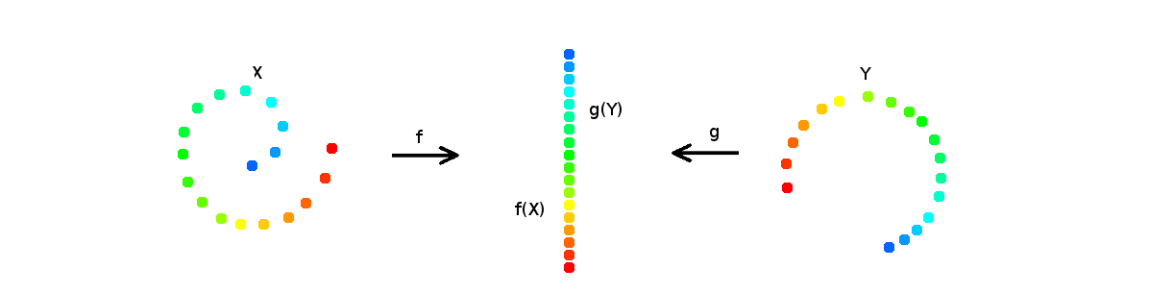
\includegraphics[width=\textwidth]{images/review/alignment.png}
    \caption{
        Figure taken from \cite{ManifoldLearningTheoryAndApplications}. The $\vecX$ and $\vecY$ spirals denote the two datasets, with the center line showing the data points embedded into the shared space, with local similarity relations being preserved. $f$ and $g$ denote the functions mapping $\vecX$ and $\vecY$ respectively into the shared space. 
    }
    % generated by analyse.py 
\end{figure}

If $f(x_i) = g(y_j)$, then $x_i$ and $y_j$ are in correspondence. If we know ahead of time that $x_i$ and $y_j$ are analogous points in their datasets, then we can provide this information to the algorithm that is trying to infer $f$ and $g$. The union of the ranges of $f$ and $g$ is then the joint latent space. This can be generalised to more than two datasets. 

This however is a definition that maps both domains into the same space. 

\subsubsection{Alignment as learning mappings from one domain to another}

In the previous definition, alignment requires that both domains be mapped to a single latent domain. This can be useful for certain problems, For example, to find a single language-independent representation of the data in multilingual related corpora. There is another definition for alignment, which requires only that domains can be mapped to each other directly. 

\begin{figure}[H]
\label{fig:alignment2}
    \centering
    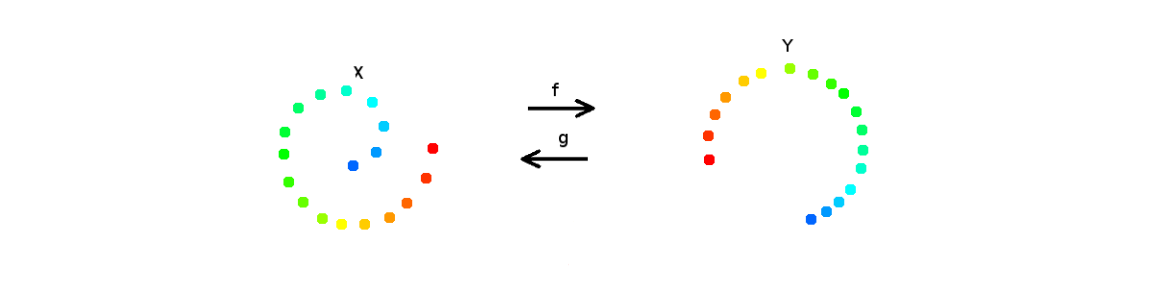
\includegraphics[width=\textwidth]{images/review/alignment2.png}
    \caption{
        The $\vecX$ and $\vecY$ spirals still denote the two datasets, but this time $f$ and $g$ denote the functions mapping $\vecX$ and $\vecY$ respectively to each other, instead of into some shared space.
    }
    % generated by analyse.py 
\end{figure}

We wish to find mappings $f(\vecX) \rightarrow \vecY$ and $g(\vecY) \rightarrow \vecX$ where the spaces $\vecX$ and $\vecY$  have similar structures. This is slightly different from the definition of alignment in the previous section. This definition may be used when it is not clear what the dimensionality of the latent space should be. 

We will use this definition of alignment in our problem, as we indeed do not know what an appropriate dimensionality should be for a latent space that represents data from both domains. 

\subsubsection{Second order isomorphism}

Returning to an idea first raised in \cite{SHEPARD19701}, we want second order isomorphism- functional relationships between clusters of concepts over the two modalities. Even if there is no structural resemblance between a concept and that concept's representation, the same structure should be observed between the relationships between the concepts  and the representations. As stated by \cite{GOLDSTONE2002295}, the meaning of a concept is tied to its relationships to other concepts in the same network. Similarity relationships between concepts within the same system can therefore be used to map between systems; using only these relationships, \cite{GOLDSTONE2002295} found an algorithm, ABSURDIST, that was able to translate between two such networks. Without constraints on the systems, or even on the number of concepts in each system, ABSURDIST was able to find translations using only similarity matrices created by some external agent (for example, a German-English bilingual human). ABSURDIST found that while within-system relationships are enough to find a translation, this translation can be made more robust to noise by adding external, extrinsic information about correspondences (for example, higher weights for certain correspondences). This is a concrete example of why the relationships between concepts are important; because they can be used to perform alignment. 

\cite{GOLDSTONE2002295} found that ABSURDIST's mappings were better for systems that had a greater number of elements. This is because such a system has more similarity relations, and each similarity relation provides a constraint to uniquely identify each member. Therefore, systems with more elements are more constrained. 

\subsubsection{Applications of alignment problems}

Some other examples of alignment problems spanning a range of applications are given below.  

\begin{itemize}
    \item Biological manifold alignment: \cite{magan} applies Generative Adversarial Networks \cite{GAN} to the problem of alignment of cell correspondence between cytometry batches.
    \item Neural style transfer: \cite{CycleGAN} takes as input differently styled source and target image sets and applies adversarial network techniques to translate images from the source set style into the target set style. 
    \item Bilingual lexical induction: \cite{wordtranslationwithoutparalleldata} applies unsupervised alignment between monolingual word representations to derive a dictionary between those languages.
    \item Deep multimodal embedding: \cite{DeepMultimodalEmbedding} relates information from three modalities- point-cloud, natural language and manipulation trajectory data, to teach a robot arm  how to manipulate new objects. 
\end{itemize}

\newpage
\subsection{Methods for concept alignment}

In this section, the following notation applies:

\begin{equation*}
\begin{split}
    &\vecX \medspace \text{denotes embeddings in the source domain},\\
    &\vecY \medspace \text{denotes embeddings in the target domain},\\
    &\vecW \medspace \text{denotes a transformation matrix}.\\
\end{split}
\end{equation*}

\subsubsection{Regression and related models}

Regression models are the simplest form of alignment model. They only require learning a transformation matrix $\vecW$ from one domain to another, minimising mean squared loss $|| (\vecW \vecX + \vecb) - \vecY||_2^2$ which can then be applied to a new source vector to map into the target space. \cite{MikolovMachineTranslation} uses this to find a ``translation matrix" that can map from word embeddings in one language space to another. Orthogonal models constrain the learned $\vecW$ matrix to be orthogonal, which is appropriate if the angles between embeddings are more important as a measure of similarity than the distances between them. Various standard preprocessing steps may be applied like normalisation to unit norm / mean centering, decorrelation to have unit variance, or SVD for dimension reduction.

Maximum margin models are similar to the support vector machine \cite{SVM} in that they balance increasing the weights from matching pairs with reducing the weights learned from known generated noise pairs. An example loss function (reproduced from \cite{kalinowski2020survey}) is:

\begin{equation*}
\begin{split}
\sumin \sum_{j \neq i}^{k} &\max \{0, \gamma - \cos(\vecW \vece_i^s, \vece_i^t) + \cos(\vecW \vece_i^s, \vece_j^t)\}\\
\spaced{with}& \vece_i, \vece_j \lspaced{being the $i$th and $j$th of $n$ embeddings},\\
& \vecW \lspaced{being the transformation matrix},\\
& k \lspaced{being the number of noise pairs}, \\
& \lspaced{and}\medspace \gamma \lspaced{being the margin parameter}.
\end{split}
\end{equation*}

This is different from regression models which rely largely on minimising the mean-squared error. \cite{Hubness} found that this form of loss reduced the effect of hubs that can plague regression and orthogonal techniques. Hubs are embeddings with high similarity to all vectors in the space, due to entities that are too common (such as words that are very frequent in a corpus) or simply as an artifact of the transformation where many features get mapped to a small region of embedding space spuriously. \cite{ImprovingSupervisedBilingualMapping} introduce another metric to reduce hubness, cross-domain similarity local scaling, that incorporates the mean of $k$-nearest neighbour distances of points in the target space to capture the neighbourhood geometry. 

Point set registration, most commonly found in computer vision, is the alignment problem applied to sets of points in 2 or 3 dimensions. \cite{PointSetRegistrationReview} reviews many current techniques; one key difference between this problem and the general alignment problem is that the points are known to lie on a 2- or 3-dimensional manifold, and this is quite a significant constraint. We cannot make any such assumptions about the dimensionality of our embeddings. 

\subsubsection{Manifold alignment models}

As stated in \cite{ManifoldLearningTheoryAndApplications}, manifold alignment is a type of constrained simultaneous dimensionality reduction with the aim of finding a low-dimensional embedding of all input datasets that preserves the topology of correspondences between them. The datasets may have disjoint features. The data may be of very high dimension, but if all the data points lie on a low-dimensional manifold, this manifold may be learnable.  

This requires the multiple datasets to be representable by a shared underlying structure. It may be convenient to learn the mappings between datasets without ever formalising this shared structure, or it may be useful to find common features. For example, in language translation it may be enough to know the mappings from words or phrases in one language to the equivalent entities in another language. However if the problem is multilingual information retrieval, it may be more useful to express the translations of different documents as a single underlying joint representation. Our specific problem is learning aligned embeddings from co-occurrence data that represent the statistics of how concepts occur in different human-created media. If we consider the ultimate underlying generative process of all these media to be ``the real world", it is plausible that the embeddings could have some underlying shared joint representation, but we do not know anything about this representation, particularly the dimensionality of the underlying process. 

Some existing dimensionality reduction techniques that can be used in alignment are the Isomap \cite{Isomap}, which reduces dimension while preserving distances between points; locally linear embedding \cite {LocallyLinearEmbedding}, which reduces dimension while keeping distances the same between local neighbourhoods; and the Laplacian eigenmap \cite{LaplacianEigenmaps}, which approximates the manifold by the adjacency graph derived from the embeddings. These algorithms all try to find a low dimensional representation of a single dataset, and manifold alignment simply uses these or similar algorithms to find embeddings for multiple datasets simultaneously. Without correspondence information, manifold alignment will result in independent embeddings for each input dataset, but if direct correspondence information is provided, or a means for inferring it, manifold alignment will use this to constrain the embeddings to be aligned. %Manifold alignment considers each individual dataset to be part of one larger dataset whose range includes the mapped values of all other datasets. 

In \cite{UnsupervisedAlignmentWP}, an approach to aligning two sets of existing embeddings (learned separately from the alignment procedure) using a combination of Procrustes analysis and the Wasserstein distance is described. Procrustes analysis is normally used to learn an affine transformation between two sets of points with a known correspondence. If we consider $\vecX \in \R^{n \times d}$ ($n$ vectors of dimension $d$) and $\vecY \in \R^{n \times d}$ (another set of vectors of the same size), the Procrustes linear transformation is the solution to the following:

\begin{equation*}
    \argmin{\vecW \in \R^{d \times d}} \quad  ||\vecX \vecW - \vecY||_2^2
\end{equation*}

\cite{Goodall1991ProcrustesMI} used this to analyse two-dimensional shapes, where the shapes are considered to be the same if by application of rotation, translation and isotropic scaling, one can be transformed to the other. \cite{MikolovMachineTranslation} applied this technique to learn linear mappings between word embeddings in different languages using a bilingual dictionary. 

The Wasserstein distance, also known as the Earth Mover Distance, is the solution of the following optimisation problem

\begin{equation*}
\begin{split}
    &\argmin{\vecP \in \mathscr{P}_n} \quad || \vecX - \vecP \vecY ||_2^2 \\
    \spaced{where}&\mathscr{P}_n = \{\vecP \in \{0, 1\}^{n \times n}, \vecP \one_n = \one_n, \vecP^T \one_n = \one_n \}
\end{split}
\end{equation*}

where $\vecP$ denotes a permutation matrix. It enforces a one-to-one mapping from the rows of $\vecX$ to $\vecY$.

%If the source and target embeddings $\vecX$ and $\vecY$ are thought of as probability distributions, $\mathscr{P}_n$ denotes a permutation matrix that moves mass from $\vecX$ to create $\vecY$. 

\cite{Zhang2017EarthMD} used this distance measure as a minimisation objective to perform automated translation without supervision. By using the Wasserstein distance as a measure of closeness between the source and target embedding spaces, they formulate a system in which minimisation of this distance draws the two distributions closer. %The translation problem faced by \cite{Zhang2017EarthMD} did not have a one-to-one mapping between symbols, because some symbols in one space map to one symbol in the other space, therefore the minimisation of the objective had to be considered over the whole distribution. 

%\cite{UnsupervisedAlignmentWP} combined both Procrustes analysis and the Wasserstein distance, to solve the following optimisation problem:

%\begin{equation*}
%\begin{split}
%\argmin{\vecQ \in \mathscr{O}_d} \quad \argmin{\vecP \in \mathscr{P}_n }\quad || \vecX \vecQ - \vecP \vecY||_2^2
%\end{split}
%\end{equation*}

%where $\vecQ$ is an orthogonal matrix. In order to practically solve this optimisation, they developed a novel stochastic algorithm to minimise a convex relaxation of this problem, details of which are omitted here. 

\subsubsection{Graph matching and graph similarity methods}

A system of interconnected concepts can be represented as a graph whose nodes represent concepts and whose edges represent relationships between concepts. For example, in \cite{Absurdist2}, such a system is represented as a directed graph with $N$ nodes whose edges are connected with labels from the set $S$ representing all combinations of possible relationships between any two nodes. Examples of such relations are ``Similar to", ``Is-A" or other hyponymic / synonymic relationships, or weights corresponding to the degree of co-occurrence of the two concepts. \cite{Absurdist2}, a sequel to \cite{GOLDSTONE2002295}, further describes how alignment of two conceptual systems may be formalised as matching two graphs.

The general graph isomorphism problem, that of telling if two graphs represent the same structure, is NP-hard \cite{GraphIsomorphismNPHard}. As cited in \cite{Absurdist2}, much work has been done in the field of finding approximate isomorphisms; finding a function $s(.)$ such that for two graphs $G_1$ and $G_2$, the distance between $s(G_1)$ and $s(G_2)$ is minimised, where $s$ is a problem-specific distance measure. There are polynomial-time algorithms for certain subtypes of graphs or trees, but in general heuristic algorithms are the only practical possibilities. 

The ABSURDIST II algorithm described in \cite{Absurdist2} creates a matrix of feasible translations between the two concept graphs which is iteratively updated based on the similarity between distances between elements of the system. At the end of the iterations, the output is a correspondence matrix that describes the strength of correspondence between elements of the source and target sets; this is used to create the mapping from source to target items. 

The \texttt{torch-two-sample} Python library and its corresponding paper \cite{torchtwosample} introduce smoothed versions of some graph-based similarity measures, such as the Friedman-Rafsky test and k-nearest neighbours test, that can be used as loss functions for learning similar graph structures. These are not actual graph isomorphism methods, but rather aim to provide distributional similarity metrics based on graph-based properties. These are converted to smooth functions by taking the statistics to be expectations of a probability distribution, thus allowing implementations to be used as loss functions trainable by backpropagation. Further details may be found in the appendix (\ref{appendix:graphbased}). 

\subsubsection{Generative adversarial networks}

The ``generative" part of a generative adversarial model is a function (usually learned by a deep learning network) that outputs samples from a distribution indistinguishable from a particular input dataset. A discriminator model is then trained against the generated outputs so that it learns to tell the difference between real and synthetic outputs; this is the ``adversarial" part. By alternating the training of these two models, the generator learns to produce better and better samples. In effect, the generator is learning to produce samples from the manifold on which the input data lies. This model was first introduced in \cite{GAN} and while the main objective is usually to generate new samples from a given distribution, there are examples where it has been used for alignment.

The Manifold Alignment GAN \cite{magan} attempts to counteract some of the problems with traditional GANs, one of them being that generated items can fool the discriminator at a batch level because the two manifolds are superimposed, rather than being aligned. When the manifolds are superimposed rather than aligned, it is as if the ``edges" of the manifolds match, but the points within may be in any position. If we were to overlay the manifolds, the corresponding points would not overlap. There are an exponential number of possible mappings that result in overlapping but unaligned manifolds. The MAGAN introduces a correspondence loss that measures the distance between a data point and its mapped image in the other domain, as well as the reconstruction loss (difference between an original point and its reconstructed image after going through both generators). %It also uses the mini-batch discrimination technique described in \cite{ImprovedTechniquesTrainingGANS} to prevent mode collapse, where all inputs get mapped to the same embedding by the generator.

%\cite{wordtranslationwithoutparalleldata} presents an adversarial method for learning cross-lingual word embeddings without supervision (without knowing beforehand any correspondences between the languages). If we consider the usual notation of $\vecX$ being the source embedding space and $\vecY$ being the target embedding space, the objective is to learn $\vecW$ such that $\vecW \vecX$ and $\vecY$ are as similar as possible. The discriminator is trained to distinguish between random samples from $\vecW \vecX$ and $\vecY$, while the generator is trained to learn $\vecW$ to prevent the discriminator from predicting accurately. They found however that the adversarial method alone did not yield better results than the supervised baseline. Therefore they also adopted a refinement procedure using Procrustes analysis to further improve the learned $\vecW$. They found that the adversarial approach would try to align all words even if they are not frequent, but the embeddings for rare words are then less frequently updated. Since the learned mapping is linear ($\vecW \vecX$) it would make sense to learn the mapping using only the most frequent words and refine afterwards. They also used the cross-domain similarity local scaling metric, which uses nearest neighbour information of each embedding to provide additional information to the optimisation.

CycleGAN \cite{CycleGAN} is not specifically an alignment model, but contains useful ideas for our purposes. CycleGAN is intended to provide image-to-image translation, where given two unordered image collections, one can be ``translated" into the style of the other. For example, transforming pictures in the style of Monet into photographic style images. CycleGAN contains two GANs; one learns a mapping $f$ from the input set $\vecX$ to the target set $\vecY$, and one learns the mapping $g$ which maps $\vecY$ to $\vecX$. A key part of the CycleGAN model is the cycle consistency loss, which for the domain $\vecX$ is $f(g(\vecY)) - \vecX$ (there is an equivalent cycle consistency loss going the other way). This loss is intended to induce $f$ and $g$ to be consistent with each other; the MAGAN model also uses this loss, calling it ``reconstruction loss". The cycle consistency / reconstruction loss is intended to reduce the possibility of the learned mapping distribution matching the output distribution, but individual inputs not being mapped to individual outputs, a different way of expressing the alignment problem. 

While GANs provide a useful basis for some alignment problems, certain types of datasets are better suited as inputs. Datasets with large numbers of object classes are not suited to GANs as they tend to underestimate the entropy in the distribution \cite{ImprovedTechniquesTrainingGANS}. Many GAN implementations take images as input, and generally the input datasets are very large, providing many samples from which to learn the appropriate distribution. Our particular dataset could be considered to have only one stimulus per concept, if we take all concepts as end nodes in the taxonomy tree.  Additionally, the salient features of images are more likely to lie on 2- or 3-dimensional manifolds. We do not know the appropriate dimensionality for the distribution that would represent any underlying manifold the concept embeddings may lie on; if the dimension of the GAN's latent space is not adequate, it will not be able to explore the sample space well, and learning will not occur. 

\section{Summary}
Regression or other similar linear algebra-based techniques are not suitable, as our source and target embeddings are of very different size (19996 concepts vs 526 concepts with an intersection of 230 concepts). While there is a one-to-one mapping between the concepts in the intersection of source and target domains, the size of this intersection set is small relative to the number of concepts in each domain, thus many concepts would be unaccounted for. 

Manifold alignment techniques dependent on mapping both domains to a shared latent space are also not considered, as we do not know anything about the dimension of this space and the wrong choice of dimensionality would greatly affect any algorithm chosen.

Graph matching, being NP-hard, is not likely to be feasible on a domain with 19996 concepts forming a complex network. Any techniques from computer vision / point set registration are unlikely to work because of the previously mentioned constraint that most of those points will lie on a 2- or 3-dimensional manifold. 

Generative adversarial networks work best when the input datasets meet certain criteria (outlined in the previous paragraph), which ours do not. However, some of the loss functions used in various GAN architectures are of interest to us, and we will make use of them when designing our approach. 




\chapter{Methodology and implementation}

\todo[inline]{Description of experiments, model architecture and reasoning behind choices. Not yet enough equations but I'm not sure how much should be included. }

\section{Dataset}

As previously mentioned, we use a dataset that represents two modalities. 

The Open Images dataset collated by Google\cite{openimages}  consists of 7337077 annotated images tagged with concepts that occur within them. Images and concepts are given IDs, and the number of occurrences of a particular concept ID in a particular image with a specific ID are recorded. We use this co-occurrence data to build a co-occurrence matrix that indicates which concepts occur together in the dataset. This is exactly analogous to the co-occurrence matrix used in \cite{pennington2014glove} from which GloVe embeddings are derived. (The dataset also contains other annotations like bounding boxes, but these are not used in this experiment)

The AudioSet dataset \cite{audioset} consists of 22160 annotated sound clips, where clips are given IDs and labelled according to which concept IDs are present in them. As this dataset is also collated by Google, the label IDs are almost the same (a small amount of preprocessing had to be done to exactly match them). Similarly to the above, a co-occurrence matrix is created from the annotation data. 

In total there are 20522 labelled concepts; 19996 from Open Images and 526 from AudioSet, with an intersection of 230 concepts present in both datasets. 

The concept labellings are both human- and machine-generated. They are not always completely accurate. For example, the image below has been labelled, by a human annotator, with the terms ``Tortoise" and ``Sea turtle". As these two terms represent distinct species, the tagged object cannot be both. In the case of this image it is presumably because the image is of a woman sitting next to a fountain in which there is a statue of a tortoise-like animal, the type of which the human tagger could not determine exactly. This pattern persists throughout the image library, where images are tagged with labels that are clearly related, but not always accurate. (In particular the Tortoise / Sea turtle mislabelling appears many times). For the purposes of this study this is less significant, but if we were trying to relate the relationships found by the experiments back to real-life data, it might be. However, the co-occurrence statistics do capture the relationships that humans think exist, even if these are inaccurate. It is a philosophical point as to whether these are accurate in a different way- that of capturing the human judgement of these relationships, even if that judgement is factually incorrect.   

In this experiment, the concept labellings have no connection to other items in the external world. In fact, the embeddings are learnt completely independently of any labellings; the embeddings are numbered by the index they occur in the co-occurrence data. For example, the first index in the Open Images co-occurrence matrix is for ``Sprenger's tulip", a type of flower, which has label ``/m/0100nhbf", but neither of these labels (the human name or the machine ID) are used anywhere in the learning system. Any ``meanings" that we ascribe to relationships between embeddings must be inferred from later re-mapping the names/IDs back to the indexes. If the system learns a system of embeddings that relate concepts 15268 and 5296 in such a way that they are close in embedding space, we will not know until later that the concepts 15268 and 5296 are ``Coffee" and ``Tea" (in which case they are related, and our algorithm is fit for purpose), or that they are ``Sprenger's tulip" and ``Ferret" (in which case they are not related). 

\begin{figure}[H]
    \centering
    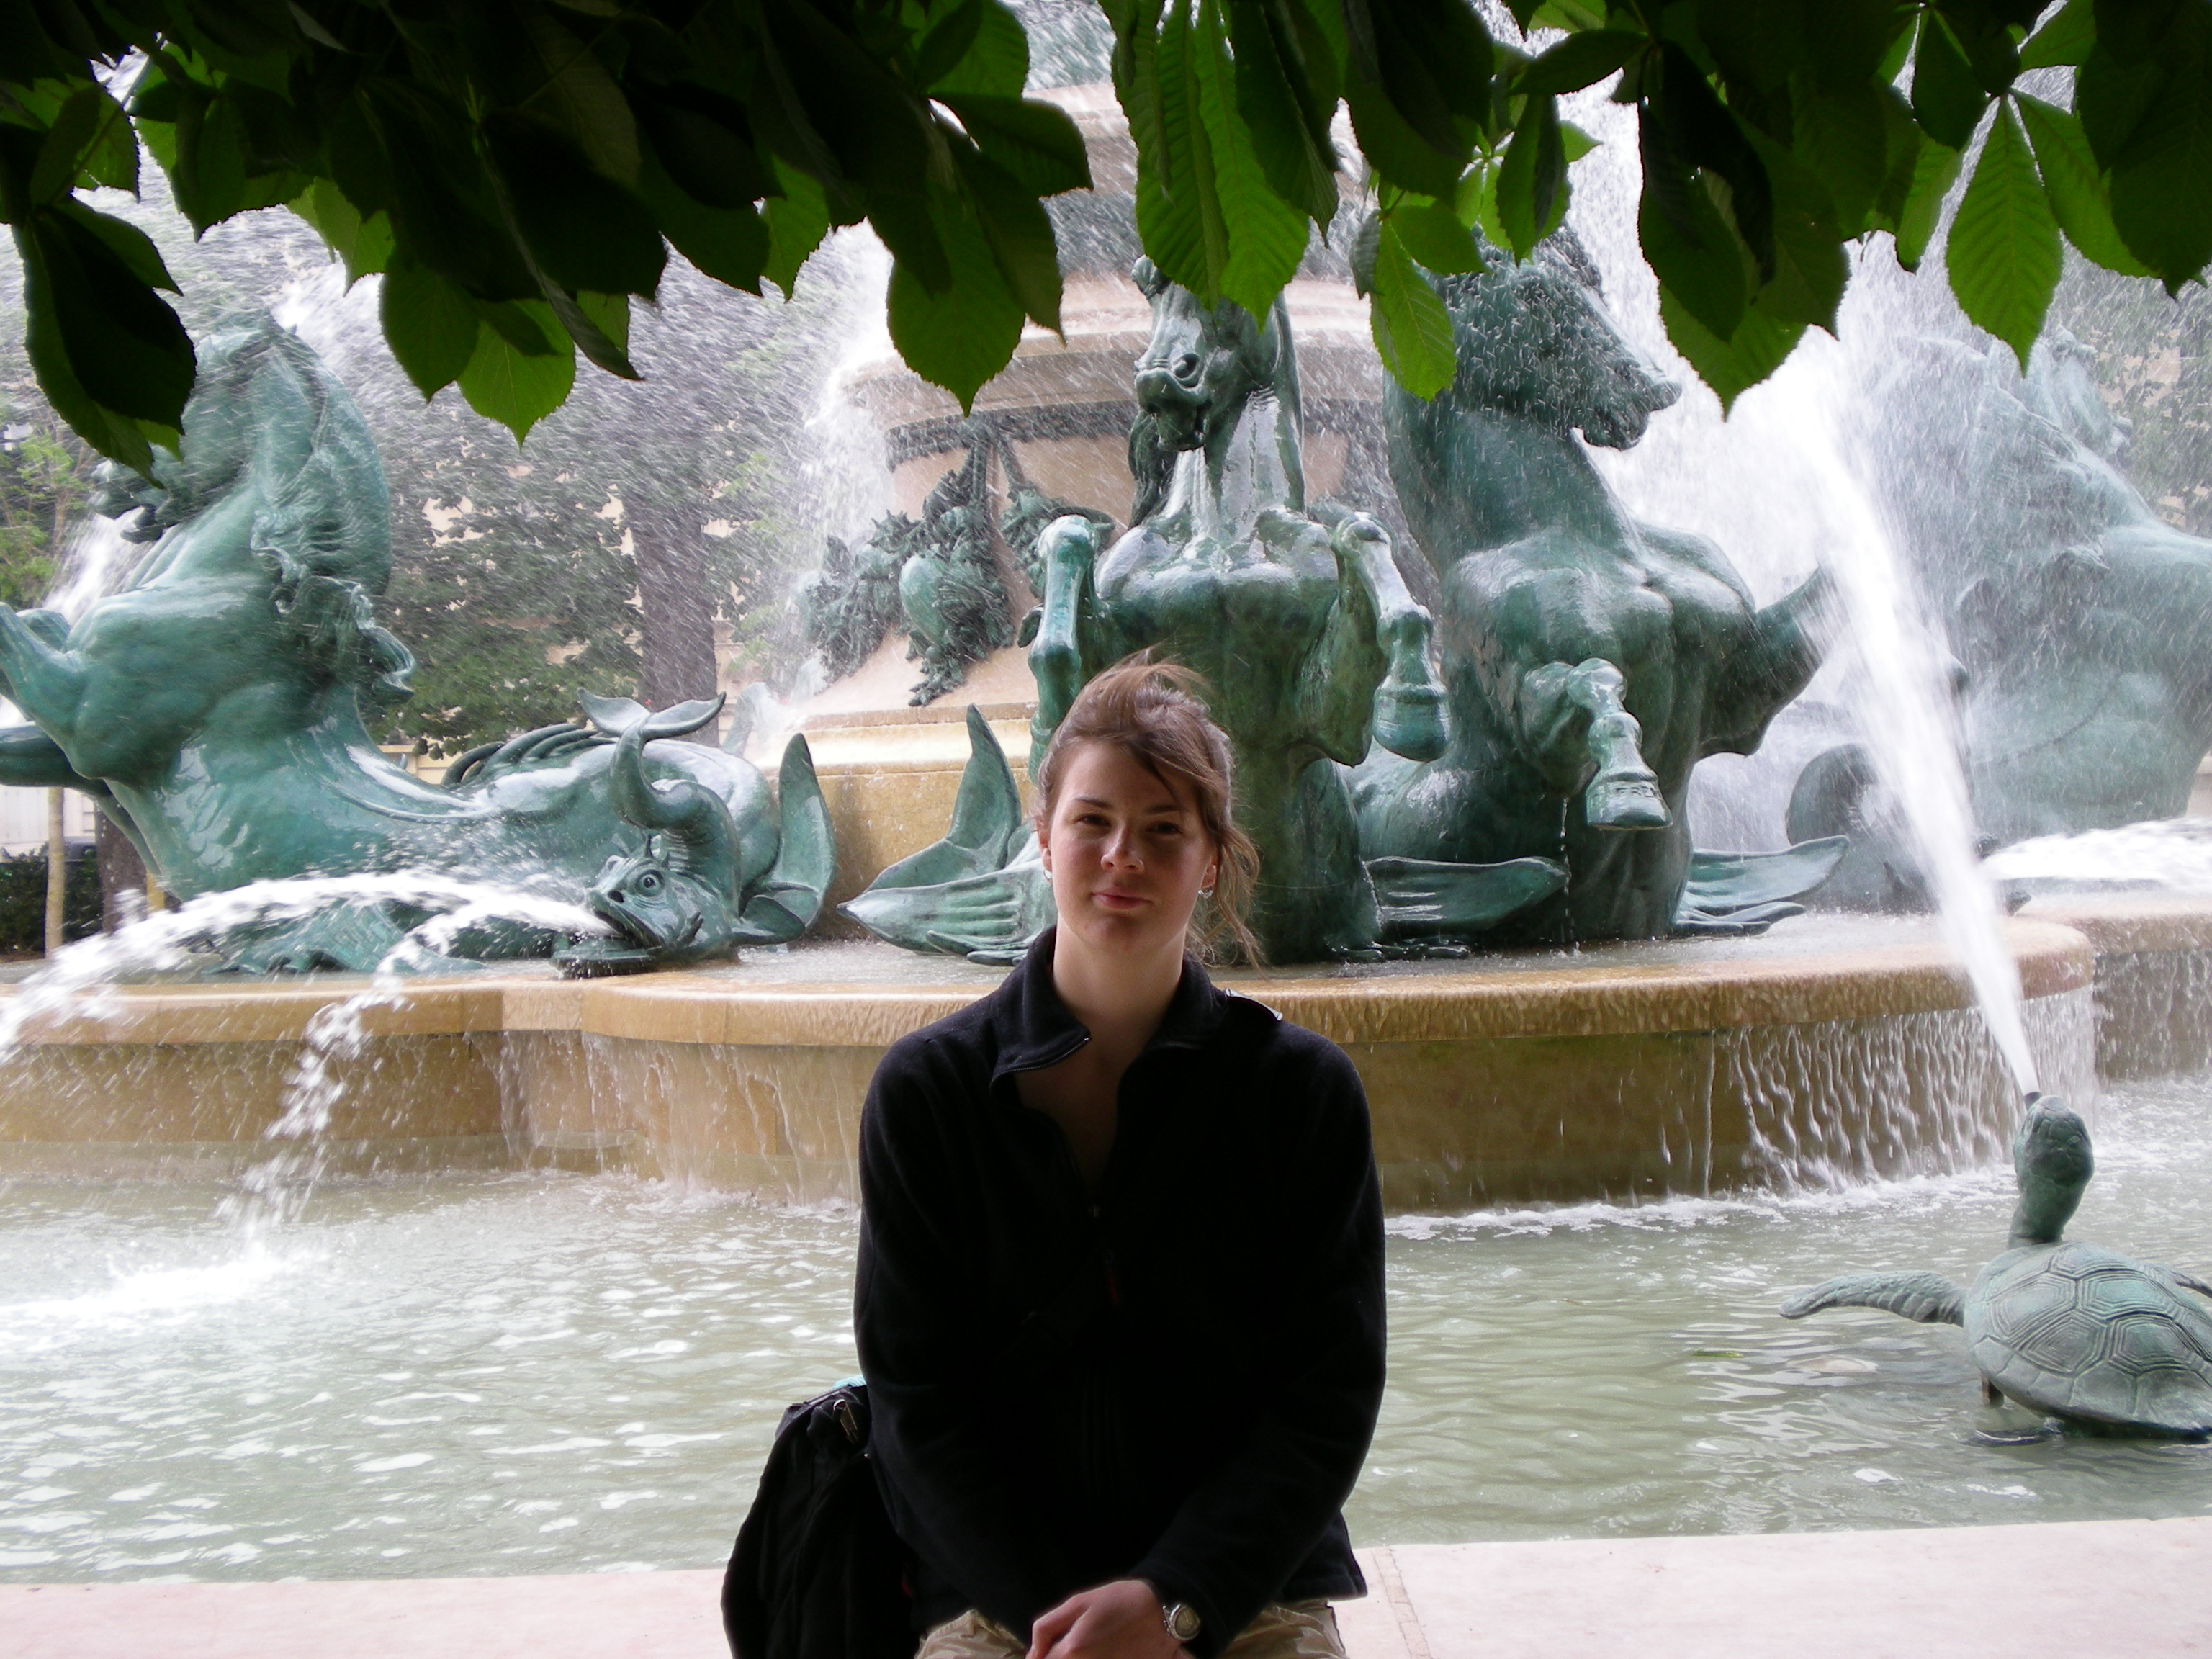
\includegraphics[width=0.95\textwidth]{images/method/tortoise_seaturtle.jpg}
    \caption{
        An image with at least one mislabelled concept: The fountain statue is labelled as both ``Tortoise" and ``Sea turtle"; it cannot be both. 
    }
\end{figure}


The co-occurrence matrices for the Open Images and AudioSet datasets, as well as the concept name to label mapping files, make up the dataset for these experiments. This dataset should represent the statistical distribution of co-occurrence of concepts in the two modalities (image and audio). \\

Other points

\begin{itemize}
    \item Both datasets also have ontology / hierarchy information
    \item Open Images: https://storage.googleapis.com/openimages/2018\_04/bbox\_labels\_600\_hierarchy\_visualizer/circle.html
    \item AudioSet: http://research.google.com/audioset/ontology/index.html
    \item Add item about how co-occurrence matrices were created and saved
\end{itemize}

\section{Choice of embeddings: Probabilistic GloVe embeddings}

As the dataset comprises co-occurrence statistics, it is similar input to that used to learn GloVe embeddings \cite{pennington2014glove}. The GloVe learning algorithm is particularly efficient, as it uses only the non-zero items in the co-occurrence matrix, which for our dataset is extremely sparse. The computational complexity of the model depends on the number of such non-zero items rather than on the size of the co-occurrence matrix. It has been found to produce reasonable clusters of concepts, that is, the concepts learnt from this algorithm are close in embedding space if they are close in semantic space. \cite{pennington2014glove} found that the embedding space produced by this algorithm gave an accuracy of 75\% on a word analogy test, which was state-of-the-art at the time of their publication. 

Stability: https://arxiv.org/pdf/2004.14876v1.pdf - number of overlaps of N nearest neighbours (usually 10) over different runs of the embeddings. 

We make two further additions to this embedding model. Firstly, we implement probabilistic embeddings; the original GloVe embeddings are deterministic. The probabilistic/deterministic distinction refers not to the learning algorithm (which has a probabilistic component as it uses minibatch gradient descent), but to the embedding representation. The original GloVe embeddings are represented by multidimensional vectors; a single vector for each concept. In our implementation, each probabilistic embedding is intended to represent a multivariate Gaussian distribution with independent dimensions (diagonal covariance matrix). 

A probabilistic embedding is a sample from the following distribution:
\begin{equation}
    \mu + \sigma \N(0, 1)
\end{equation}

Both $\mu$ and $\sigma$ are learnt parameters. In practice, $\sigma$ is further parametrised as follows, to enforce positivity:

\begin{equation}
    \sigma = \ln (1 + \exp (\rho))
\end{equation}

Therefore the full equation for a probabilistic embedding is 

\begin{equation}
\label{eq:stochemb}
    \mu + \ln (1 + \exp(\rho)) \cdot \N(0, 1)
\end{equation}

\subsection{Implementation}

A probabilistic version of the GloVe learning algorithm was implemented in Python using the PyTorch \cite{pytorch}, PyTorch Lightning \cite{pytorchlightning} and Pyro \cite{pyro} libraries. Specifically, a custom neural network layer was implemented which took as input a co-occurrence matrix, and learnt probabilistic GloVe embeddings based on iterating over the concepts represented in the matrix. Each mini-batch represented a random sampling of the rows and columns of the co-occurrence matrix, with all rows and columns being used over the course of one training epoch. 

The GloVe loss function is reproduced here:

\begin{equation}
\label{eq:gloveloss}
\begin{split}
L &= \sum_i \sum_j f(X_{ij}) (w_i^T w_j + b_i + b_j - \log X_ij)^2\\
f(x) &= \begin{cases}
(x/x_{max})^{\alpha}\spaced{if} x \le x_{max}\\
1\spaced{otherwise}
\end{cases}
\end{split}
\end{equation}

\begin{itemize}
    \item The values of hyperparameters $\alpha = 0.75$ and $x_{max} = 100$  are set as in the original paper, \cite{pennington2014glove}. 
    \item The $X_{ij}$ are samples of the current probabilistic embeddings represented by equation \ref{eq:stochemb}. 
\end{itemize}

The Pyro library provides backpropagation through the random sampling, as described in \cite{deeplearninggoodfellow} (section 20.9). The next section describes how these probabilistic embeddings were verified. 

\subsection{Validation}

The probabilistic embeddings were validated as follows:

\begin{itemize}
    \item Train embeddings learnt from Open Images and AudioSet co-occurrence data. 
    \item Each domain's embeddings are learnt individually without regard for alignment. 
    \item For each run of each domain, the random seed was manually set. 10 seeds were used in total capturing 10 separate embeddings for each domain. 
    \item The following learning parameters were used:
    \begin{itemize}
        \item Embedding dimension of 6. This choice was heuristic: the test implementation of GloVe embeddings implemented in PyTorch had 1 million unique tokens and dimensionality of 300, to keep the same ratio of effective tokens to dimensionality, 6 was the closest integer. 
        \item Mini-batch size of 500
        \item The Adam \cite{kingma2017adam} optimiser, with learning rate 0.01
        \item 250 epochs of training for Open Images and 2000 epochs for AudioSet. This was enough to ensure convergence of the GloVe loss decreasing to asymptotic levels. 
        \begin{itemize}
            \item It is interesting that AudioSet needed many more epochs to converge. This is consistent with an earlier point mentioned in \cite{GOLDSTONE2002295} that systems with more concepts are easier to learn as they are more constrained. 
        \end{itemize}
    \end{itemize}
    \item No hyperparameter tuning was done; as this is not a supervised learning problem, we measure convergence only by the decrease in GloVe loss (equation \ref{eq:gloveloss}). Overfitting does not occur and the GloVe loss decreases steadily to an asymptotic value. 
\end{itemize}

The output of this training are 10 sets of probabilistic embeddings (parametrised by their mean and variance) for each domain (Open Images / AudioSet). These embeddings are doubly stochastic; one source is stochasticity in the learning algorithm leading to 2 runs with different seeds converging to different mean embeddings, and the other is caused by each embedding being a sample from a multivariate Gaussian distribution. 

\subsubsection{Clustering}
As a sanity check, the t-SNE (t-Distributed Stochastic Neighbor Embedding, \cite{tsne}) algorithm was  used to reduce the dimensionality of the embeddings from 6 to 2, and the resulting points plotted for the top 300 most frequently occurring concepts in each domain (measured by number of occurrences in images or audio clips). As we expected, there are clear clusters of concepts visible. This clustering was visible over different seeds. While t-SNE adds a further level of stochasticity during the dimensionality reduction process, two runs of t-SNE on the same input data with the same t-SNE random seed set, will produce the same result. Therefore, we can assume that the stochasticity introduced by t-SNE is accounted for. 

This is a qualitative analysis only intended to confirm that the implementation is correct and converges to embeddings that have sensible semantic relationships. This technique of using t-SNE to sanity check embedding quality is commonly used in other similar experiments (for example \cite{CoocurrenceVisionLanguage2021}). 

\begin{figure}[H]
    \centering
    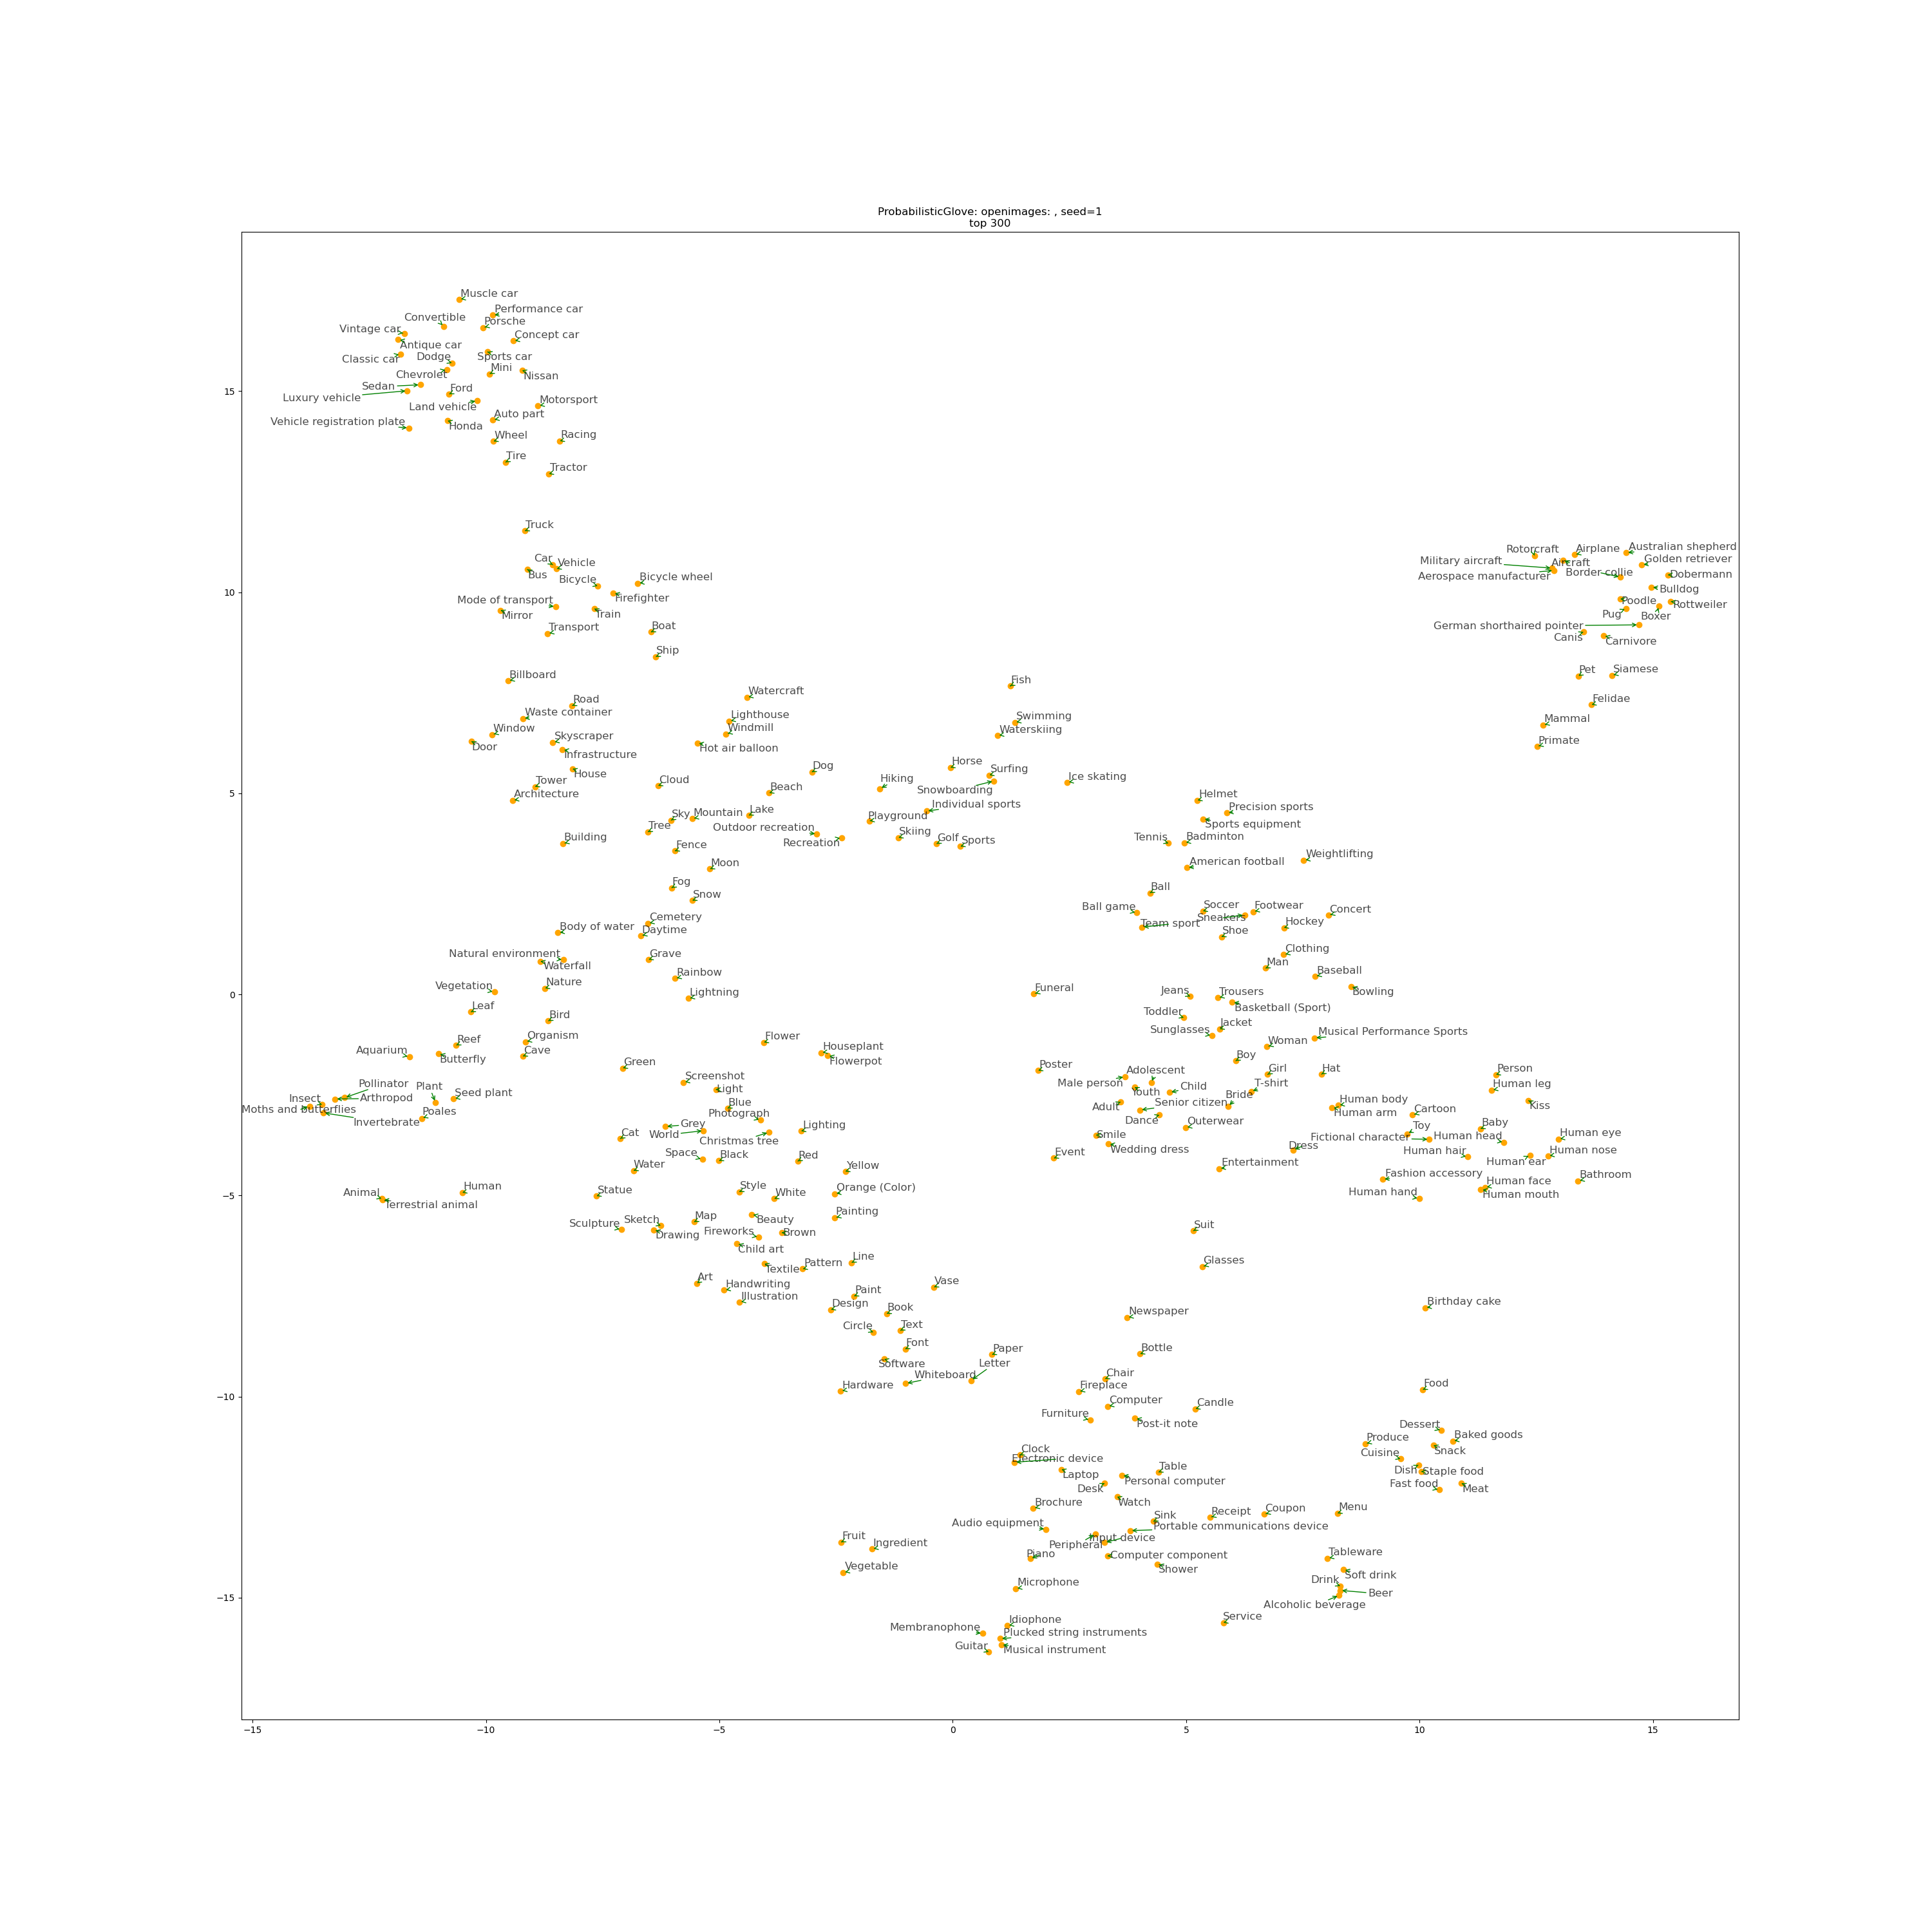
\includegraphics[width=1.0\textwidth]{images/method/probabilistic_independent/top300_tsne_openimages__ProbabilisticGlove_1.png}
    \caption{
        Open Images top 300 most common concepts. There are clearly visible clusters corresponding to, amongst other things, different types of dog, different types of vehicle, and different types of human body part. Blue points correspond to concepts present in both Open Images and AudioSet. Orange points correspond to the top 300 most frequently occurring concepts in the Open Images dataset (that are not also in the intersection of concepts).
    }
    % generated by inspect_results.py 
\end{figure}

\begin{figure}[H]
    \centering
    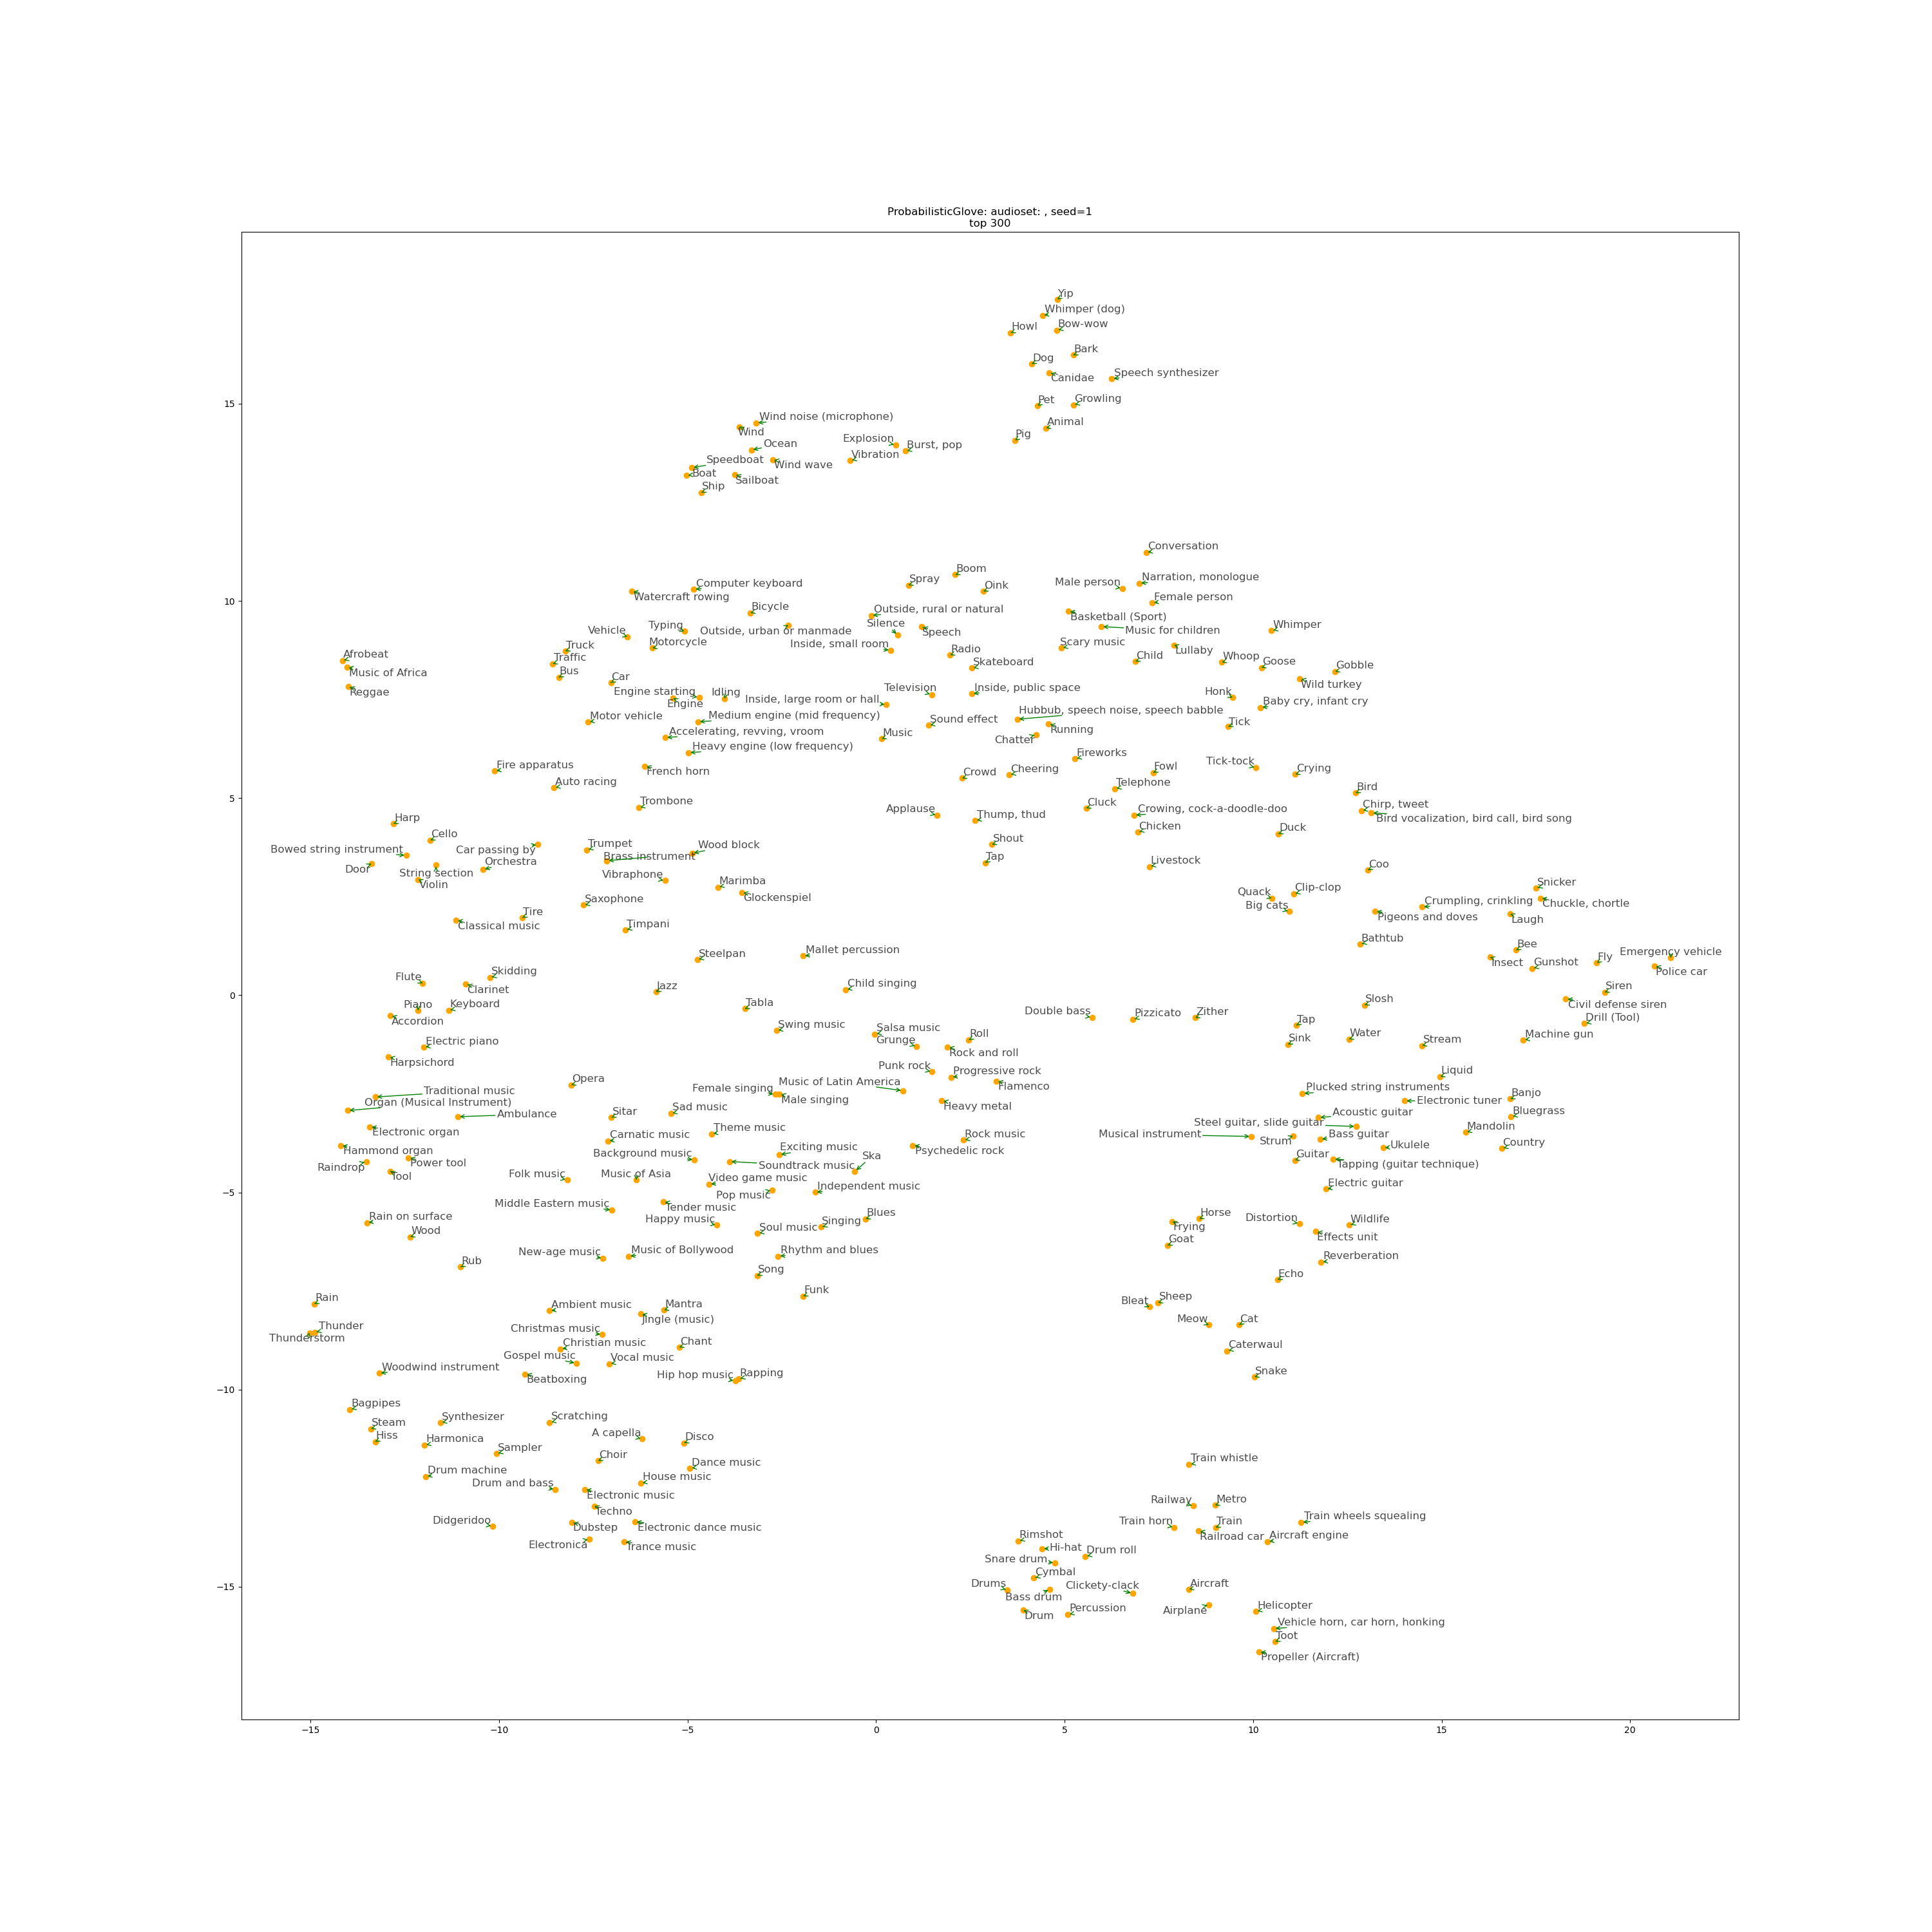
\includegraphics[width=1.0\textwidth]{images/method/probabilistic_independent/top300_tsne_audioset__ProbabilisticGlove_1.png}
    \caption{
        AudioSet top 300 most common concepts. Again there are clearly visible clusters comprising, for example, sounds made by water, sounds made by percussion instruments, and sounds made by dogs. Blue points correspond to concepts present in both Open Images and AudioSet. Orange points correspond to the top 300 most frequently occurring concepts in the AudioSet dataset (that are not also in the intersection of concepts).
    }
    % generated by inspect_results.py 
\end{figure}

Plots of the Open Images top 300 concepts t-SNE plots annotated to show the clusters, for random seeds 1 and 2, show that roughly the same concepts cluster for each run. They also reveal a characteristic of our alignment problem: The cluster arrangements relative to each other across runs are not consistent. Ideally, we would like the different clusters to have the same spatial arrangement across runs. As described in \cite{SHEPARD19701}, we would like to identify second order isomorphisms in the data; not just the clusters, but the relationship between the clusters. 

\begin{figure}[H]
    \centering
    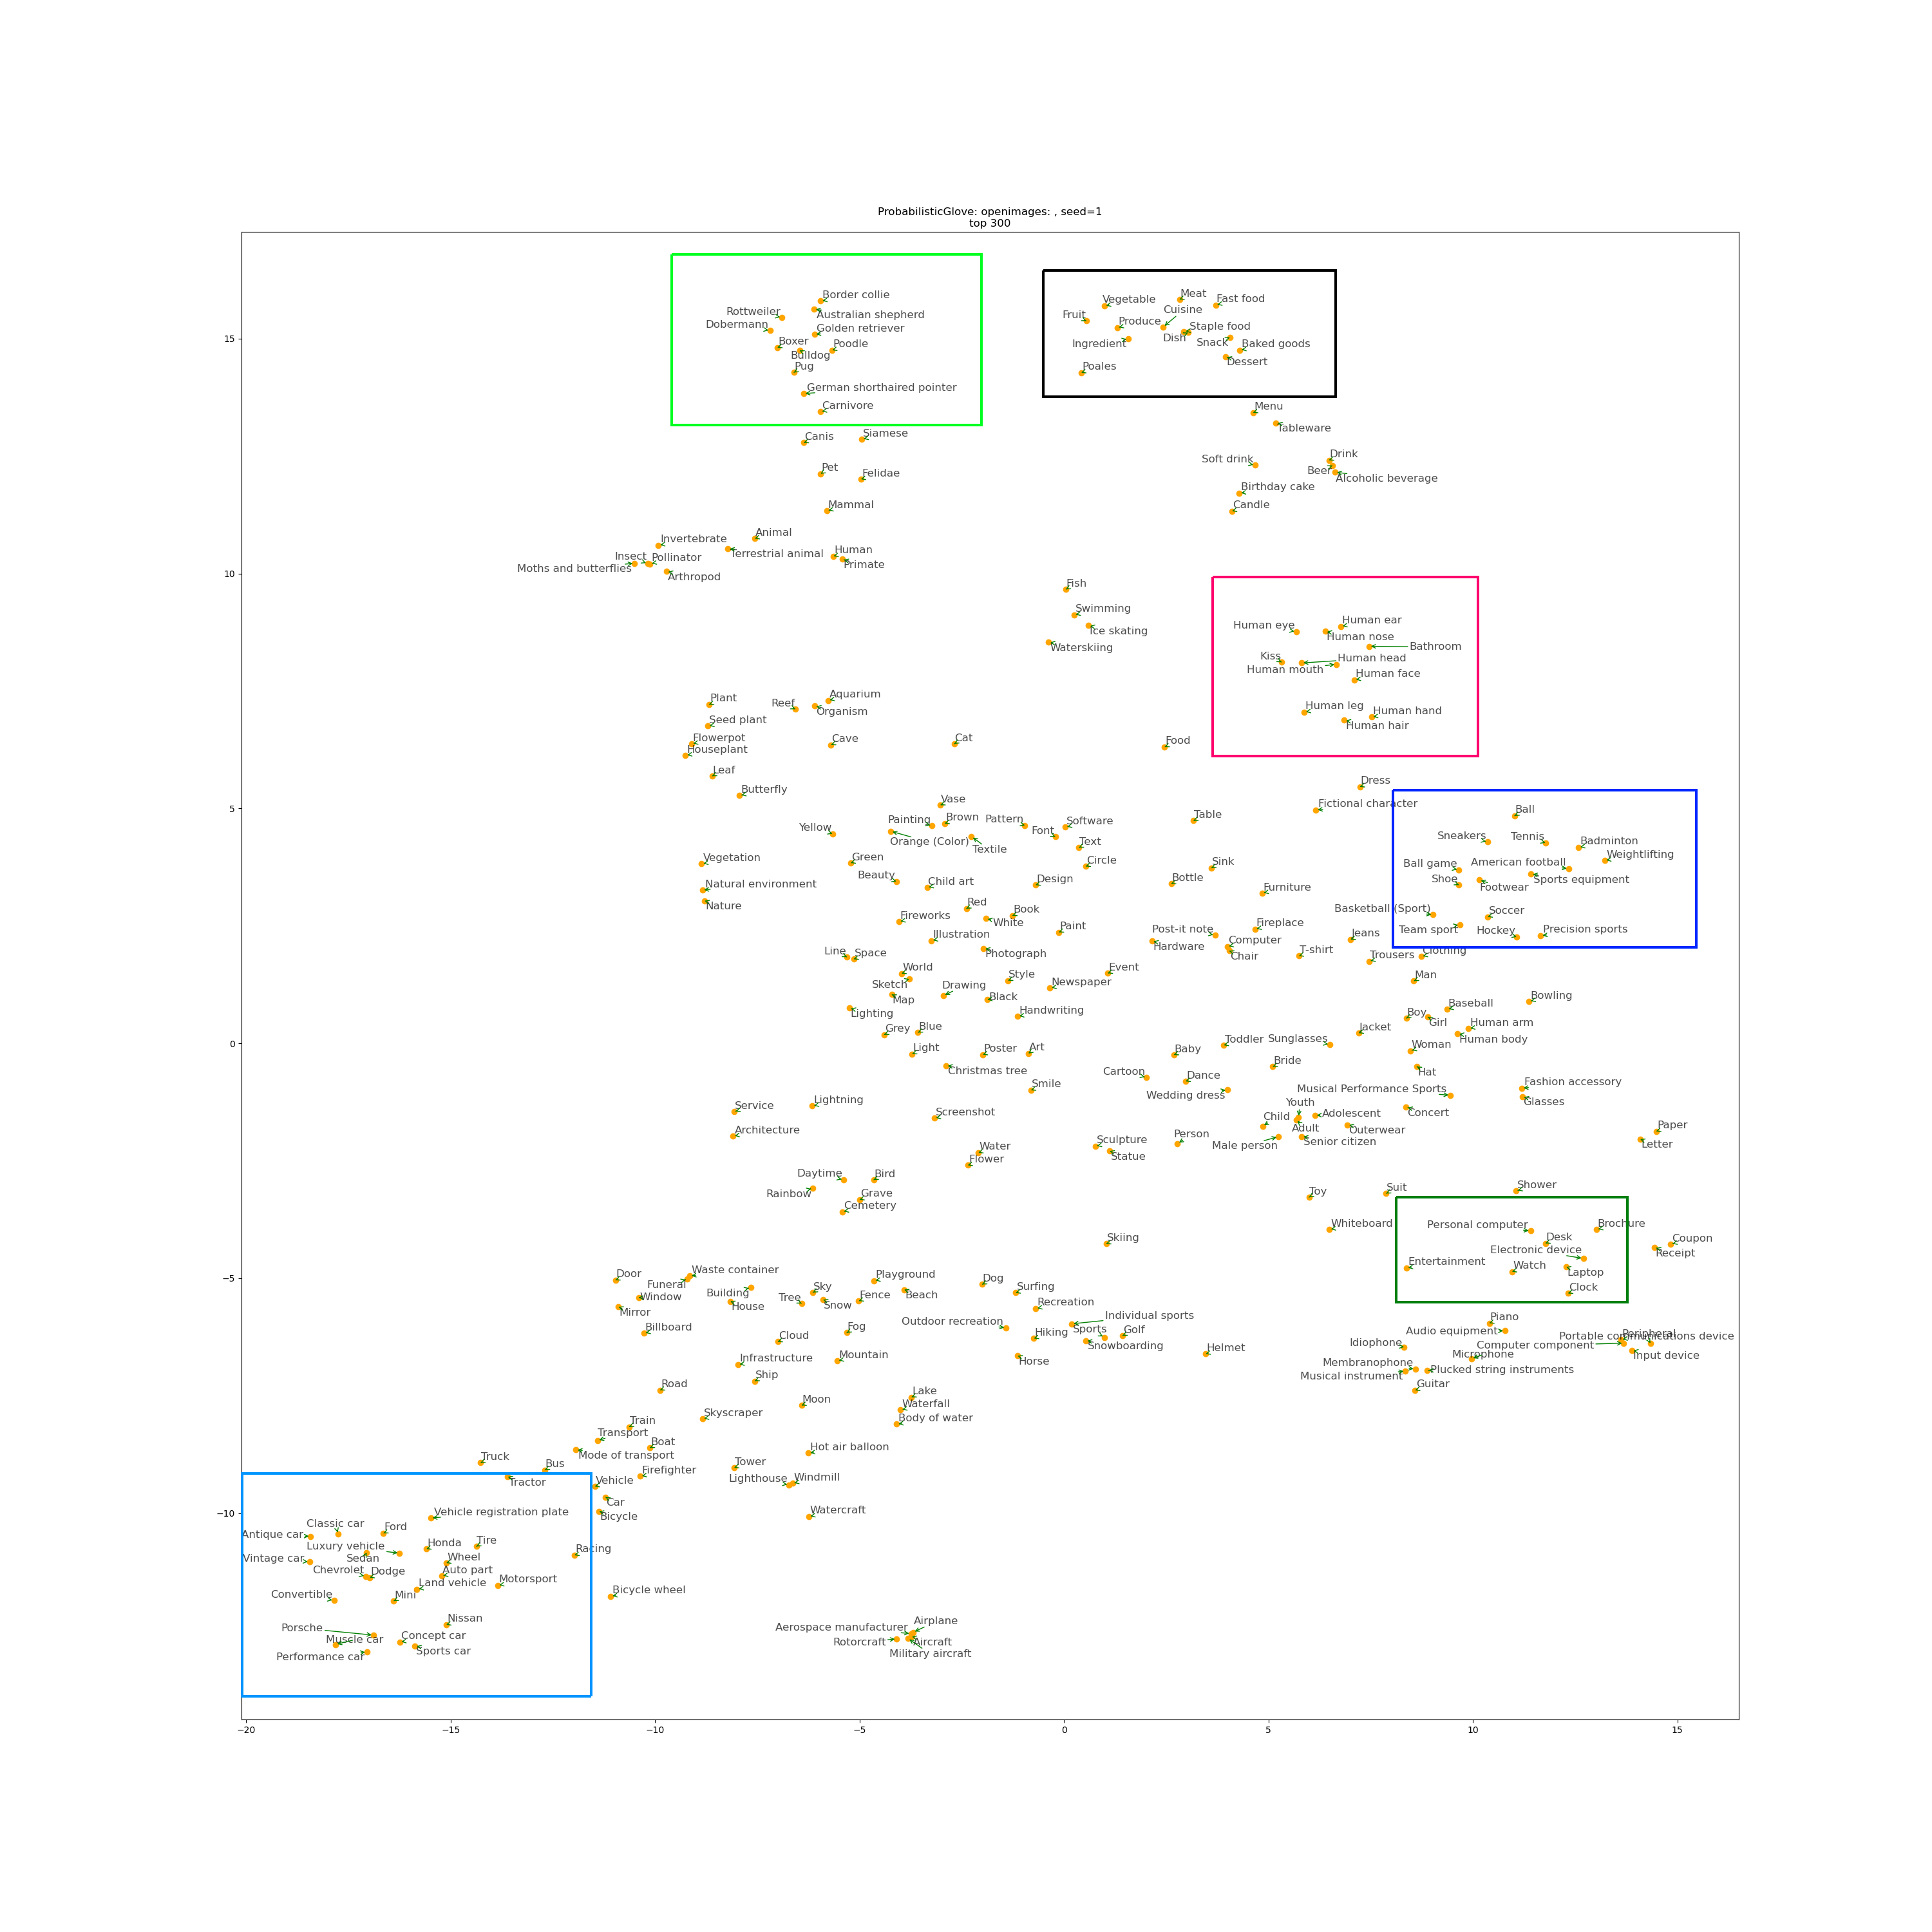
\includegraphics[width=0.95\textwidth]{images/method/probabilistic_independent/top300_tsne_openimages__ProbabilisticGlove_1_clusters.png}
    \caption{
        Coloured boxes indicate clusters 
    }
    % generated by inspect_results.py 
\end{figure}

\begin{figure}[H]
    \centering
    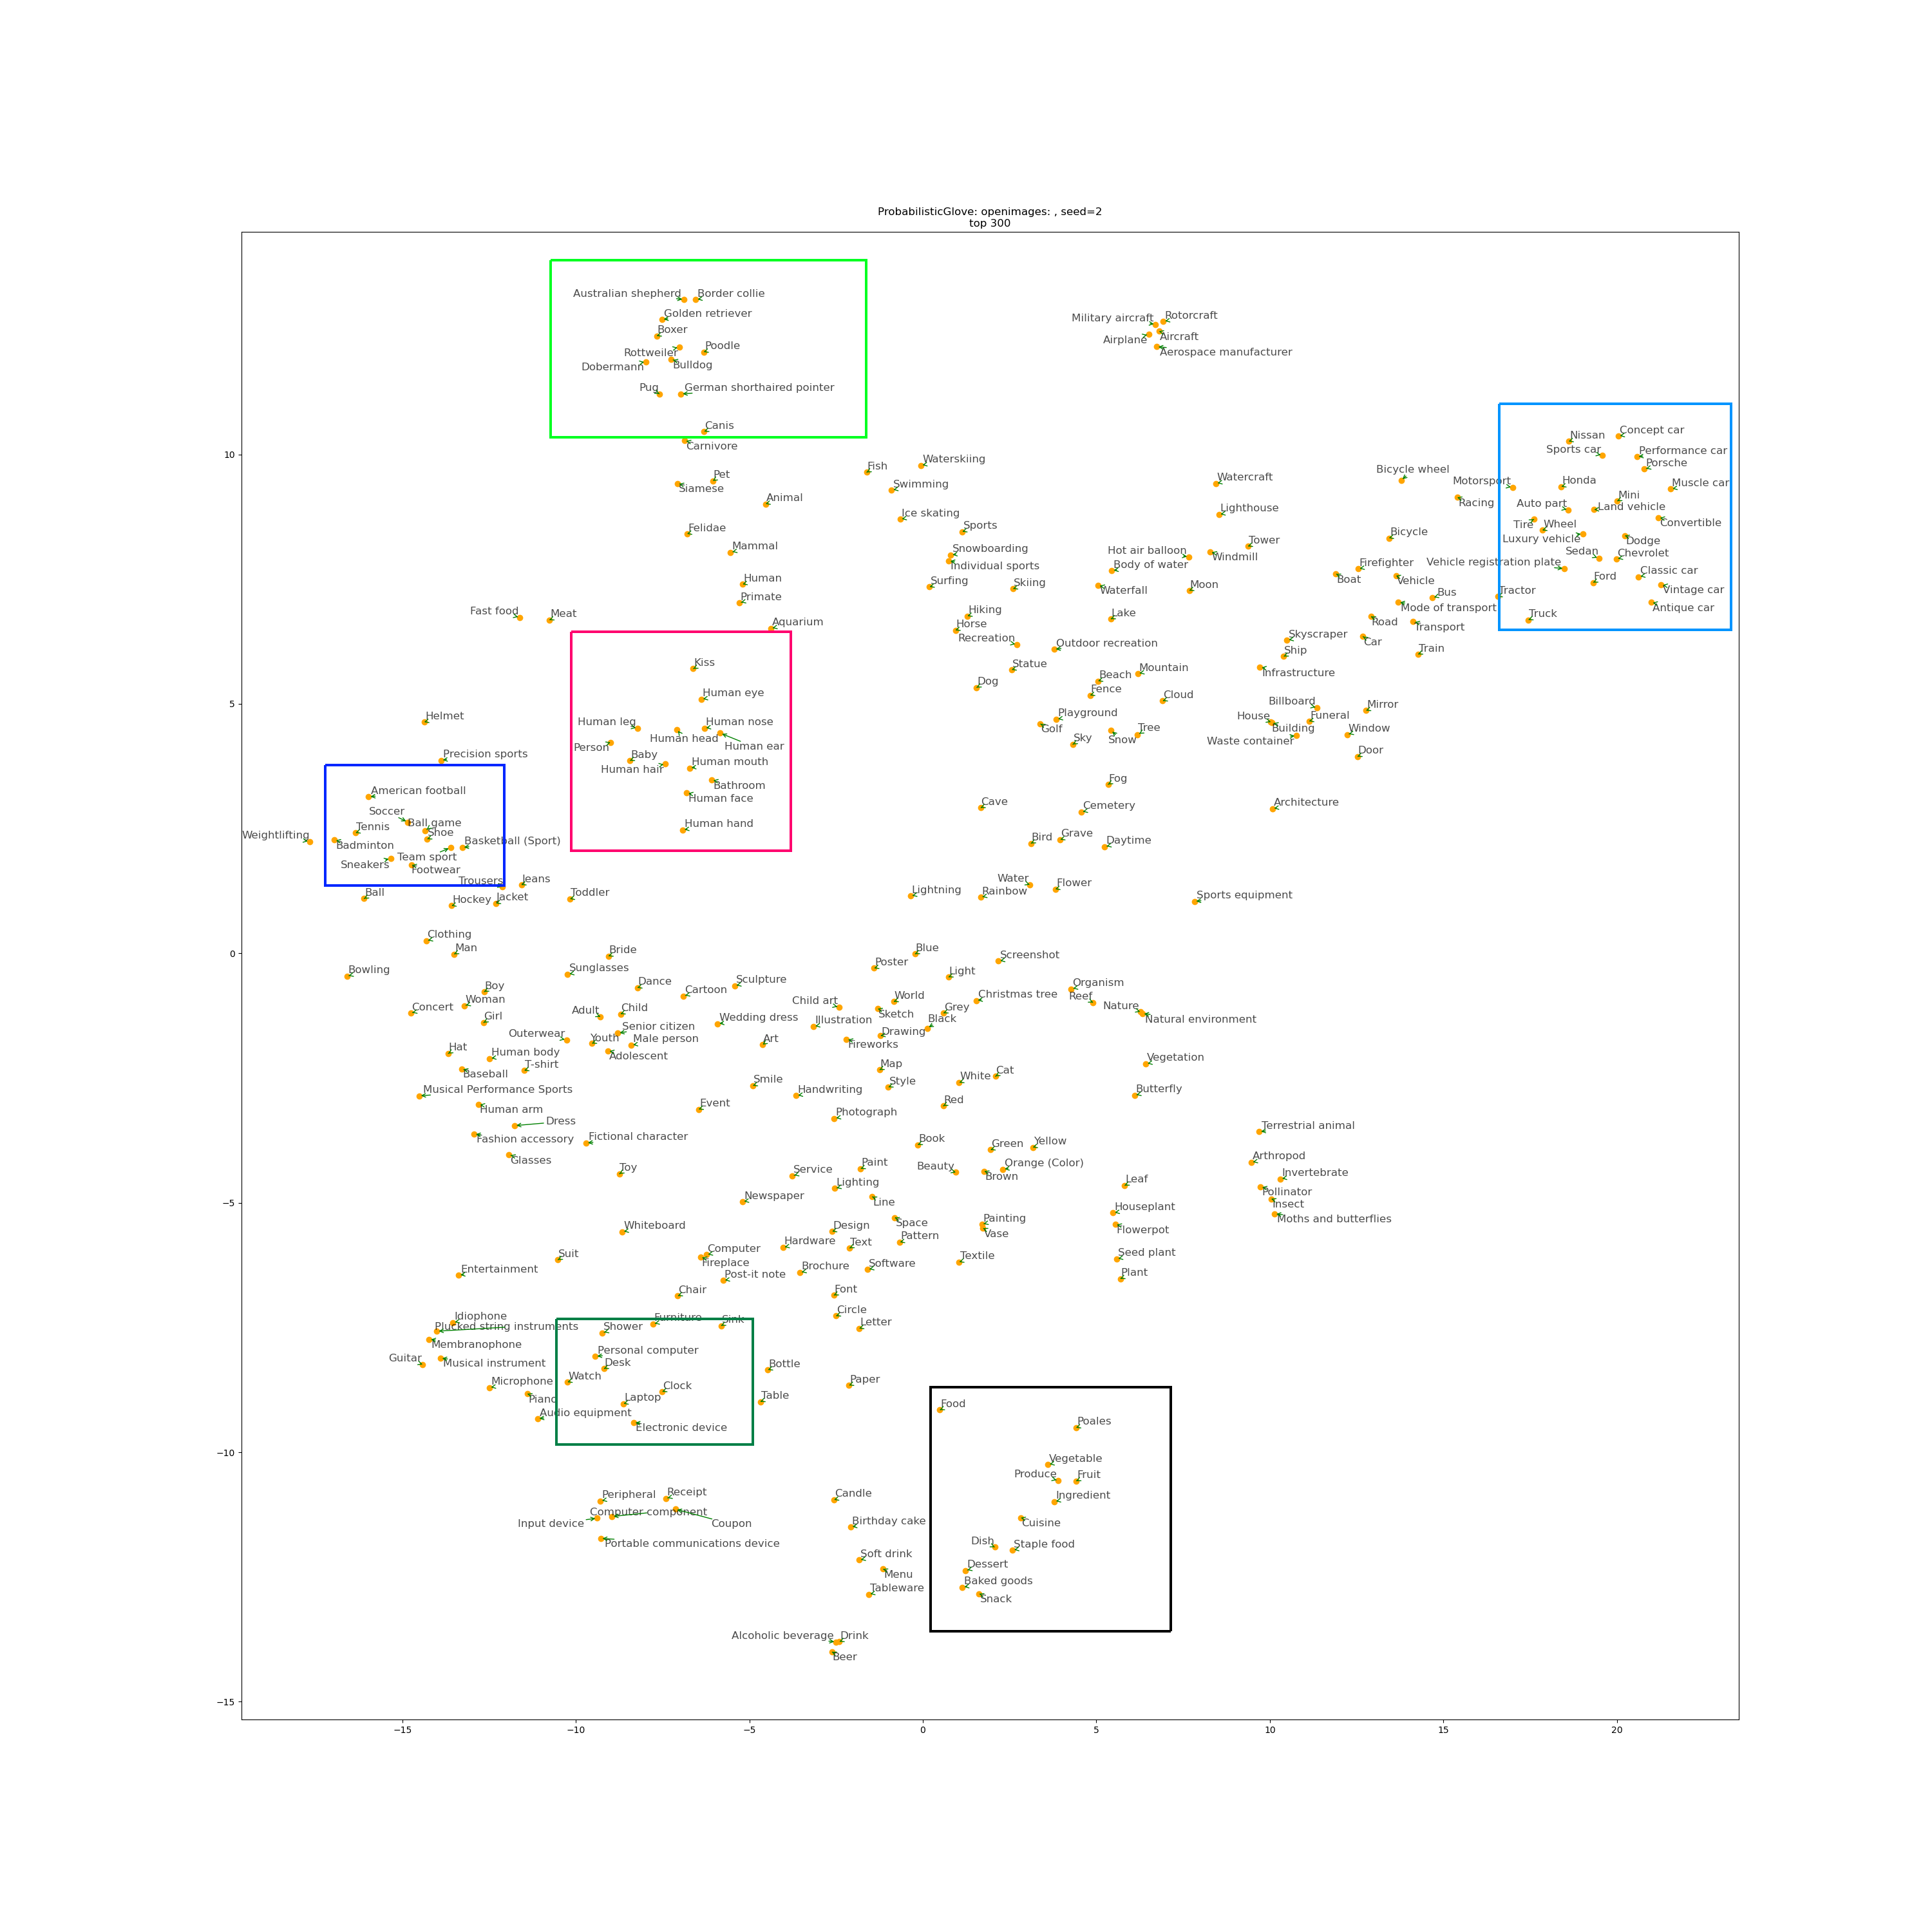
\includegraphics[width=0.95\textwidth]{images/method/probabilistic_independent/top300_tsne_openimages__ProbabilisticGlove_2_clusters.png}
    \caption{
        The same clusters are in different locations in embedding space compared to the previous run, and their orientation relative to each other is different; it is not a simple rotation and stretch of the clusters. Although t-SNE introduces more stochasticity, both t-SNE runs were done with the same t-SNE random seed set, which is known to generate the same output if given the same inputs. 
    }
    % generated by inspect_results.py 
\end{figure}

\subsubsection{Learnt parameters of the probabilistic embeddings}

We also examine the learnt means and variances, $\mu$ and $\sigma = \ln(1 + \exp(\rho))$, of each embedding. 

This is done as follows for each domain (Open Images and AudioSet separately):

\begin{itemize}
    \item Dot product distances are calculated between the learnt $\mu$ (the mean of the stochastic embeddings) for every pair of concepts. Since the stochastic embeddings can be thought of as distributions about a mean, where the mean would be the embedding learnt in the deterministic case. 
    \item This gives a similarity matrix between each embedding and itself, for each seed. 
    \item The correlation between the values of each run's similarity matrix with every other run was computed, and the mean value taken. A high value should indicate that the concepts in each run have the same similarity with each other. 
    \item This was $ \pm $ for AudioSet and $0.9989 \pm 8.5261e-06$ for OpenImages. 
% /home/petra/spond/spond/experimental/glove/results/audioset/ProbabilisticGlove/audioset_analytics.hdf5
% /home/petra/spond/spond/experimental/glove/results/openimages/ProbabilisticGlove/openimages_analytics.hdf5
\end{itemize}

The variances were examined by analysing the entropy of each embedding. Since each embedding is a multivariate Gaussian with a diagonal covariance matrix:

\begin{equation}
\begin{split}
H(x) &= \frac{1}{2} \ln |\Sigma| + \frac{D}{2}(1 + \ln(2 \pi))\\
&= \frac{1}{2} \ln \prod_{i=1}^D \sigma_i + \frac{D}{2}(1 + \ln(2 \pi))\\
\end{split}
\end{equation}

In the above, $\sigma_i$ is the variance for dimension $i$. 
 
By examining histograms of the entropies of each run (with different seeds), we can check if the algorithm is producing stable results. 
\begin{figure}[H]
    \centering
    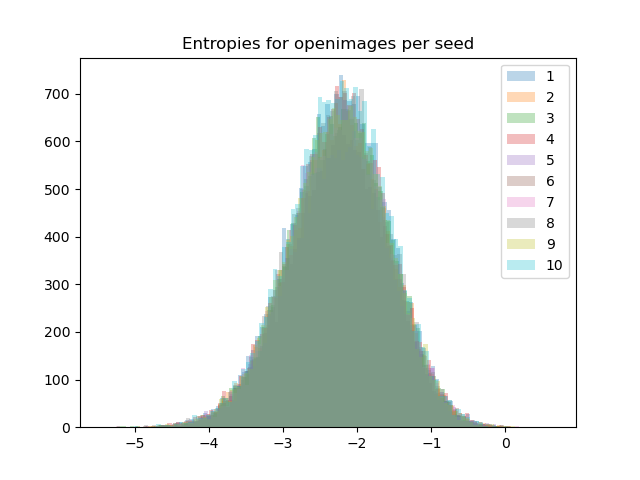
\includegraphics[width=0.9\textwidth]{images/method/probabilistic_independent/openimages_entropies.png}
    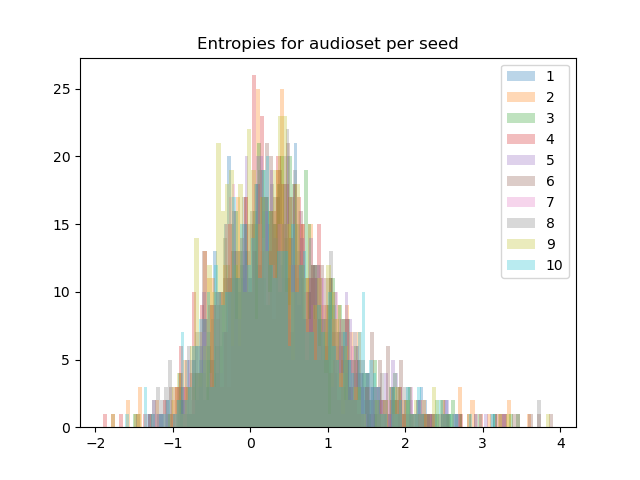
\includegraphics[width=0.9\textwidth]{images/method/probabilistic_independent/audioset_entropies.png}
    \caption{
        Histograms of entropy distributions for Open Images and AudioSet embeddings. 
    }
    % generated by analyse.py 
\end{figure}
 
The histograms indicate that the distributions of the variances of learned embeddings are stable even if the random seed is changed. The AudioSet graph is less smooth because there are only 526 concepts vs. 19996 in Open Images. 
 
We expect that concepts with lower incidence (that are present fewer times in the universe of images / audio clips) should have a higher variance, and therefore higher entropy. This is confirmed by calculating the Spearman correlation of the entropies with the number of incidences of a concept. For AudioSet, this results in a mean Spearman correlation of -0.3465 over 10 random seeds, and for Open Images this is a mean of -0.3369 over 10 random seeds. 

\todo[inline]{We also have the correlation with the deterministic embeddings. Does it mean anything? }

\todo[inline]{Run stability calculation eg. how many of 5-nearest neighbour are present in different runs of same seed, top 200 concepts. }
% audioset
%In [8]: det_learnt_corr.mean()
%Out[8]: 0.9189375433154889
%
%In [9]: entropy_count_rcorr.mean()
%Out[9]: 
%spearmanr   -3.465071e-01
%p            7.865913e-14
%dtype: float64


% openimages
%In [5]: det_learnt_corr.mean()
%Out[5]: 0.2926545426484884
%In [6]: entropy_count_rcorr.mean()
%Out[6]: 
%spearmanr   -0.336871
%p            0.000000
%dtype: float64


% For the following, run inspect_results.py and call mostalike to dump top 5 neighbours for a few seeds
% then 

The table below shows the 3 nearest neighbours (in the rows) to the concept ``Cat" in the Open Images domain, over five seeds. The distance metric is Euclidean distance. There is a consistency to the items, but they do not appear to be very related to the concept of ``Cat".  

    \begin{table}[]
    \begin{tabular}{@{}llll@{}}
Rank / Seed &1 &2 &3 \\
\toprule
1&\begin{tabular}[c]{@{}l@{}} Rope \\ 0.290 \end{tabular}&\begin{tabular}[c]{@{}l@{}} Cage \\ 0.257 \end{tabular}&\begin{tabular}[c]{@{}l@{}} Totem pole \\ 0.392 \end{tabular} \\
2&\begin{tabular}[c]{@{}l@{}} Surfing \\ 0.302 \end{tabular}&\begin{tabular}[c]{@{}l@{}} Human \\ 0.306 \end{tabular}&\begin{tabular}[c]{@{}l@{}} Sketch \\ 0.422 \end{tabular} \\
3&\begin{tabular}[c]{@{}l@{}} Hammock \\ 0.302 \end{tabular}&\begin{tabular}[c]{@{}l@{}} Mammal \\ 0.403 \end{tabular}&\begin{tabular}[c]{@{}l@{}} Peace symbols \\ 0.429 \end{tabular} \\
4&\begin{tabular}[c]{@{}l@{}} Picnic table \\ 0.364 \end{tabular}&\begin{tabular}[c]{@{}l@{}} Fawn \\ 0.412 \end{tabular}&\begin{tabular}[c]{@{}l@{}} Beach \\ 0.429 \end{tabular} \\
5&\begin{tabular}[c]{@{}l@{}} Screenshot \\ 0.394 \end{tabular}&\begin{tabular}[c]{@{}l@{}} Vertebrate \\ 0.421 \end{tabular}&\begin{tabular}[c]{@{}l@{}} Outdoor furniture \\ 0.438 \end{tabular} \\

    \end{tabular}
    \end{table}



This table shows the 5 nearest neighbours to the concept ``Domestic short-haired cat" in the Open Images domain, also over 3 seeds. This looks a lot more sensible. 


    \begin{table}[]
    \begin{tabular}{@{}llll@{}}
Rank / Seed &1 &2 &3 \\
\toprule
1&\begin{tabular}[c]{@{}l@{}} Malayan cat \\ 0.100 \end{tabular}&\begin{tabular}[c]{@{}l@{}} Malayan cat \\ 0.083 \end{tabular}&\begin{tabular}[c]{@{}l@{}} Malayan cat \\ 0.144 \end{tabular} \\
2&\begin{tabular}[c]{@{}l@{}} Burmese \\ 0.195 \end{tabular}&\begin{tabular}[c]{@{}l@{}} Russian blue \\ 0.118 \end{tabular}&\begin{tabular}[c]{@{}l@{}} Himalayan \\ 0.183 \end{tabular} \\
3&\begin{tabular}[c]{@{}l@{}} Russian blue \\ 0.215 \end{tabular}&\begin{tabular}[c]{@{}l@{}} Bombay \\ 0.229 \end{tabular}&\begin{tabular}[c]{@{}l@{}} Russian blue \\ 0.200 \end{tabular} \\
4&\begin{tabular}[c]{@{}l@{}} Abyssinian \\ 0.228 \end{tabular}&\begin{tabular}[c]{@{}l@{}} Polydactyl cat \\ 0.237 \end{tabular}&\begin{tabular}[c]{@{}l@{}} Bengal \\ 0.238 \end{tabular} \\
5&\begin{tabular}[c]{@{}l@{}} Tabby cat \\ 0.240 \end{tabular}&\begin{tabular}[c]{@{}l@{}} Ragdoll \\ 0.256 \end{tabular}&\begin{tabular}[c]{@{}l@{}} Tabby cat \\ 0.267 \end{tabular} \\

    \end{tabular}
    \end{table}


\todo[inline]{It is a known weakness of Euclidean embeddings to represent hierarchical concepts. Hyperbolic / Poincare embeddings may be needed. }


\todo[inline]{Is it possible to relate the results to the entropies? It is often the more specific terms that have more sensible nearest neighbours. This is the opposite of what I expected when looking at the entropies.}

We observe that often, the more specific terms in the domain have more sensible nearest neighbours. For example, these are the 5 nearest neighbours to the concept ``Roti canai", which is a very specific type of Malaysian flatbread. The nearest neighbours are extremely specific and accurate; ``Roti prata", ``Paratha" and ``Uttapam" are all types of Asian flatbread. 

    \begin{table}[]
    \begin{tabular}{@{}llll@{}}
Rank / Seed &1 &2 &3 \\
\toprule
1&\begin{tabular}[c]{@{}l@{}} Roti prata \\ 0.222 \end{tabular}&\begin{tabular}[c]{@{}l@{}} Roti prata \\ 0.264 \end{tabular}&\begin{tabular}[c]{@{}l@{}} Roti prata \\ 0.145 \end{tabular} \\
2&\begin{tabular}[c]{@{}l@{}} Tortilla de patatas \\ 0.235 \end{tabular}&\begin{tabular}[c]{@{}l@{}} Roti \\ 0.299 \end{tabular}&\begin{tabular}[c]{@{}l@{}} Pastelón \\ 0.329 \end{tabular} \\
3&\begin{tabular}[c]{@{}l@{}} Pastelón \\ 0.244 \end{tabular}&\begin{tabular}[c]{@{}l@{}} Paratha \\ 0.303 \end{tabular}&\begin{tabular}[c]{@{}l@{}} Timballo \\ 0.340 \end{tabular} \\
4&\begin{tabular}[c]{@{}l@{}} Paratha \\ 0.287 \end{tabular}&\begin{tabular}[c]{@{}l@{}} Uttapam \\ 0.315 \end{tabular}&\begin{tabular}[c]{@{}l@{}} Pastitsio \\ 0.350 \end{tabular} \\
5&\begin{tabular}[c]{@{}l@{}} Timballo \\ 0.360 \end{tabular}&\begin{tabular}[c]{@{}l@{}} Naan \\ 0.358 \end{tabular}&\begin{tabular}[c]{@{}l@{}} Bobotie \\ 0.376 \end{tabular} \\

    \end{tabular}
    \end{table}



\section{Alignment techniques}

\subsection{Definition of alignment for this problem}

As stated in \cite{ManifoldLearningTheoryAndApplications}, the alignment problem involves finding a transformation of one dataset that maps it to another. 

The $x$- and $y$-embeddings (Open Images and AudioSet respectively) are considered to be aligned if the following holds:

\begin{itemize}
    \item For every member of the set $x_{intersect} = y_{intersect}$ of concepts that exist in both domains, the nearest neighbour of mapped concept $f(x_i)$ is the corresponding member $y_i$ in set $y_{intersect}$, and the nearest neighbour of mapped concept $g(y_i)$ is the corresponding member $x_i$ in set $x_{intersect}$. 
\end{itemize}

The accuracy is computed after each epoch of training. It is defined as the fraction of concepts (only in the intersection set) in a domain whose nearest neighbour after mapping is the known other embedding in that domain. 

\subsection{Alignment network}

The alignment network comprises the following:

\begin{itemize}
    \item A probabilistic GloVe embedding layer representing the first domain of embeddings to be aligned (henceforth referred to as the x-embeddings). In the case of these experiments, this is Open Images. 
    \item A probabilistic GloVe embedding layer representing the second domain of embeddings to be aligned (henceforth referred to as the y-embeddings). In the case of these experiments, this is AudioSet. 
    \item A multi-layer perceptron with 3 hidden layers of 100 nodes each, that learns a mapping from the x-embeddings to the y-embeddings: $f(x) \rightarrow y$
    \item A multi-layer perceptron with 3 hidden layers of 100 nodes each, that learns a mapping from the y-embeddings to the x-embeddings: $g(y) \rightarrow x$
\end{itemize}

\todo[inline]{DIAGRAM}

\subsubsection{Full loss function}
\begin{itemize}
    \item The GloVe loss for $x$ as in \ref{eq:gloveloss}. 
    \item The GloVe loss for $y$ as in \ref{eq:gloveloss}. 
    \item The cycle consistency loss from x to y: $||g(f(x)) - y||_2$
    \item The cycle consistency loss from y to x: $||f(g(y)) - x||_2$
    \item The distance loss between $f(x)$ and $y$: difference between the mapped $x$ embeddings and the current $y$ embeddings, for only the intersection of concepts: $||f(x_{intersect}) - y_{intersect}||_2$
    \item The difference between $g(y)$ and $x$: the mapped $y$ embeddings and the current $x$ embeddings, for only the intersection of concepts: $||g(y_{intersect}) - x_{intersect}||_2$
    \item An optional distributional similarity measure between $f(x_{intersect})$ and $y_{intersect}$
    \item An optional distributional similarity measure between $g(y_{intersect})$ and $x_{intersect}$
\end{itemize}

where $x_{intersect}$ and $y_{intersect}$ represent the embeddings in both domains of the intersection of concepts between those domains. 

\subsubsection{Other model parameters}

\begin{itemize}
    \item Mini-batch size 500
    \item 10 samples of each concept embedding are taken for each mini-batch for a total of 5000 points per mini-batch
    \item Alignment accuracy is defined as: for $x$, the number of $i$ such that nearest neighbour of $f(x_i)$ is  $y_i$. For $y$, the number of $i$ such that the nearest neighbour of $g(y_i)$ is $x_i$. 
    \item The model is run for 150 epochs; the mean accuracy (over $x$ and $y$) is measured after every epoch and the model is saved if the mean accuracy is greater than the last epoch mean accuracy.
    \item The Adam optimiser is used with a learning rate of 0.01.
    \item No hyperparameter tuning is done. 
\end{itemize}

In the next sections, the individual items in the loss are discussed more thoroughly.

\subsection{GloVe loss}
\todo[inline]{Summarise loss section of GloVe paper}

Experimentally, it was found that the GloVe loss had to be scaled by the ratio of concepts: there are 19996 Open Images concepts and 526 Audioset concepts, so the $x$ glove loss (Open Images) is multiplied by 19996 / 526. Without this, the GloVe loss was not enough to result in sensible clusters. 


\subsection{Cycle consistency}

We relate a domain's mapped embeddings (through the $f(x)$ and $g(y)$ MLP layers) to the other domain using what is referred to as cycle-consistency loss. This uses transitivity to self-supervise training; we want $g(f(x))$ to be close to $x$ and $f(g(y))$ to be close to $y$. 

In \cite{CycleGAN}, the reason for requiring cycle consistency is stated: Simply requiring $f(x)$ to be close to $y$ and $g(y)$ to be close to $x$ is insufficient as overfitting can result in a network being able to map an arbitrary set of inputs to an arbitrary set of outputs. In \cite{CycleGAN}, the L1 norm is used, in this experiment we use the L2 norm as we do not want a sparsity constraint. 

Thus the cycle consistency loss takes the following form:

\begin{equation}
\begin{split}
L_{cycle} &= E_x ||f(g(x)) - x||_2 + E_y ||g(f(y) - y||_2
\end{split}
\end{equation}

This loss is also used in other alignment architectures, for example \cite{magan} (in which it is known as the reconstruction loss). 


\subsection{Distance loss}

This measures how far away the mapped embedding is from the original embedding. This loss represents the semi-supervised component of the algorithm; it is only calculated for items in the intersection of the 2 concept domains (the 230 concepts present in both Open Images and AudioSet, for our problem). 
\begin{equation}
\begin{split}
L_{distance} &= E_x||f(x) - y||_2 + E_y||g(y) - x||_2
\end{split}
\end{equation}

\todo[inline]{There is something about this in the MAGAN paper \cite{magan}}

\subsection{Distributional similarity}

We would like the distribution of $f(x)$ to be similar to the distribution of $y$, and that of $g(y)$ to be similar to that of $x$. For the intersection of concepts, this means that the distribution of $f(x_{intersect})$ should be similar to $y_{intersect}$, and the distribution of $g(y_{intersect})$ should be similar to $x_{intersect}$. There exist various measures by which two distributions can be compared; for these to be used as loss functions for neural network training, they should generate a scalar value that is minimised when the distributions are identical. 

\todo[inline]{Introduce distance measures?}

\subsubsection{Maximum mean discrepancy}

The maximum mean discrepancy (MMD) statistic is introduced in \cite{MMDGretton} as a difference in feature means of the two distributions, where the features are obtained by applying a kernel function to the two samples. Under certain conditions met by the kernel function, the MMD between samples of 2 distributions is 0 if the distributions are identical. Summarising the full theory that can be found in \cite{MMDGretton}, the following conditions must hold:

\begin{itemize}
    \item The kernel must be a characteristic kernel: If the inputs are random variables $X$ with domain $\Omega$ and distribution $P$, there is a one to one mapping between the mean value in feature space and the distributions. \cite{KernelMeanEmbeddingReview} \todo[inline]{ADD EQUATIONS? Unclear how much proof is needed}
    \item That is, each value for the mean in feature space maps to a different possible distribution. 
    \item An intuitive way of looking at this is that the kernel function must be "rich enough" to represent all possible distributions. A known characteristic kernel function that is commonly used is the Gaussian kernel function $k(\vecx, \vecy) = \exp(-\alpha ||\vecx - \vecy||_2^2)$, and this is what we use in our experiments. 
    \item $\alpha$ of 0.01 was used for both domains. This value was chosen because it is close to the median of the pairwise distances \todo[inline]{Find citation for median heuristic} which is a good heuristic for convergence. 
\end{itemize}

Other random bits

\begin{itemize}
    \item MMD with a characteristic kernel will be 0 if the distributions are the same and certain conditions are met of the embedding space. 
    \item MMD is like infinite moment matching, if a characteristic kernel is used. 
\end{itemize} 

Given the following:

\begin{itemize}
    \item $\vecx_i$ are $m$ samples from one distribution  $X$
    \item $\vecy_j$ are $n$ samples from the other distribution $Y$
    \item $k(\vecx, \vecx')$ is a characteristic kernel function
\end{itemize}

The empirical unbiased MMD statistic is as follows:

\begin{equation}
\label{eq:mmd}
\begin{split}
MMD (k, x, y) &= \frac{1}{m(m-1)} \sumim \sum_{j \neq i}^m k(\vecx_i, \vecx_j) + \frac{1}{n(n-1)} \sumin \sum_{j \neq i}^n k(\vecy_i, \vecy_j) \\
&- \frac{2}{mn} \sumim \sumjn k(\vecx_i, \vecy_j)
\end{split}
\end{equation}

It can be seen that this is the sum of the within-distribution similarities, less the sum of the cross-distributional similarities. 

(Can include more items described in http://ssa.cf.ac.uk/big-data/slides/Gretton-MMD-TrainingNetworks.pdf)

(Empirical MMD can be negative)

The implementation from the \texttt{torch-two-sample / https://torch-two-sample.readthedocs.io} library \cite{torchtwosample} was used.  




\chapter{Results}

In this chapter we present the results of semi-supervised learning of jointly aligned embeddings, where ``jointly aligned" means that embeddings for both domains and the mapping from one to the other are all learned simultaneously. 


\section{Summary}
\begin{itemize}
    \item Alignment accuracies of greater than 95\% were achieved for both domains ($f(x) \rightarrow y$ and $g(y) \rightarrow x$).
    \item Visualisation of the jointly aligned embeddings through t-SNE dimensionality reduction showed good clustering behaviour with semantically meaningful clusters.
    \item Aligned embeddings were found to be of higher quality compared to independently learned embeddings, when using a similarity metric based on the WordNet lexical database. Specific definitions of ``quality" and ``similarity" are given in a later section.
    \item Aligned embeddings were found to be less stable compared to independently learned embeddings. 
    \item The MMD metric increased alignment accuracy, but sometimes decreased embedding quality. 
\end{itemize}


\section{Visualising clusters}
Similar to what was done with the independently learned embeddings, we run the t-SNE algorithm on the aligned embeddings for both domains, and plot the results.

In Figures \ref{fig:openimagesaligned} and \ref{fig:audiosetaligned} below, the blue points represent the concepts in the intersection i.e. they are present in both Open Images and AudioSet. The orange points represent the concepts that are in the 300 most frequent for the respective domain that are not also in the intersection. Only the t-SNE plots for alignment run without MMD are shown, as the plots for alignment run with MMD look materially similar. 

\begin{figure}[H]
    \centering
    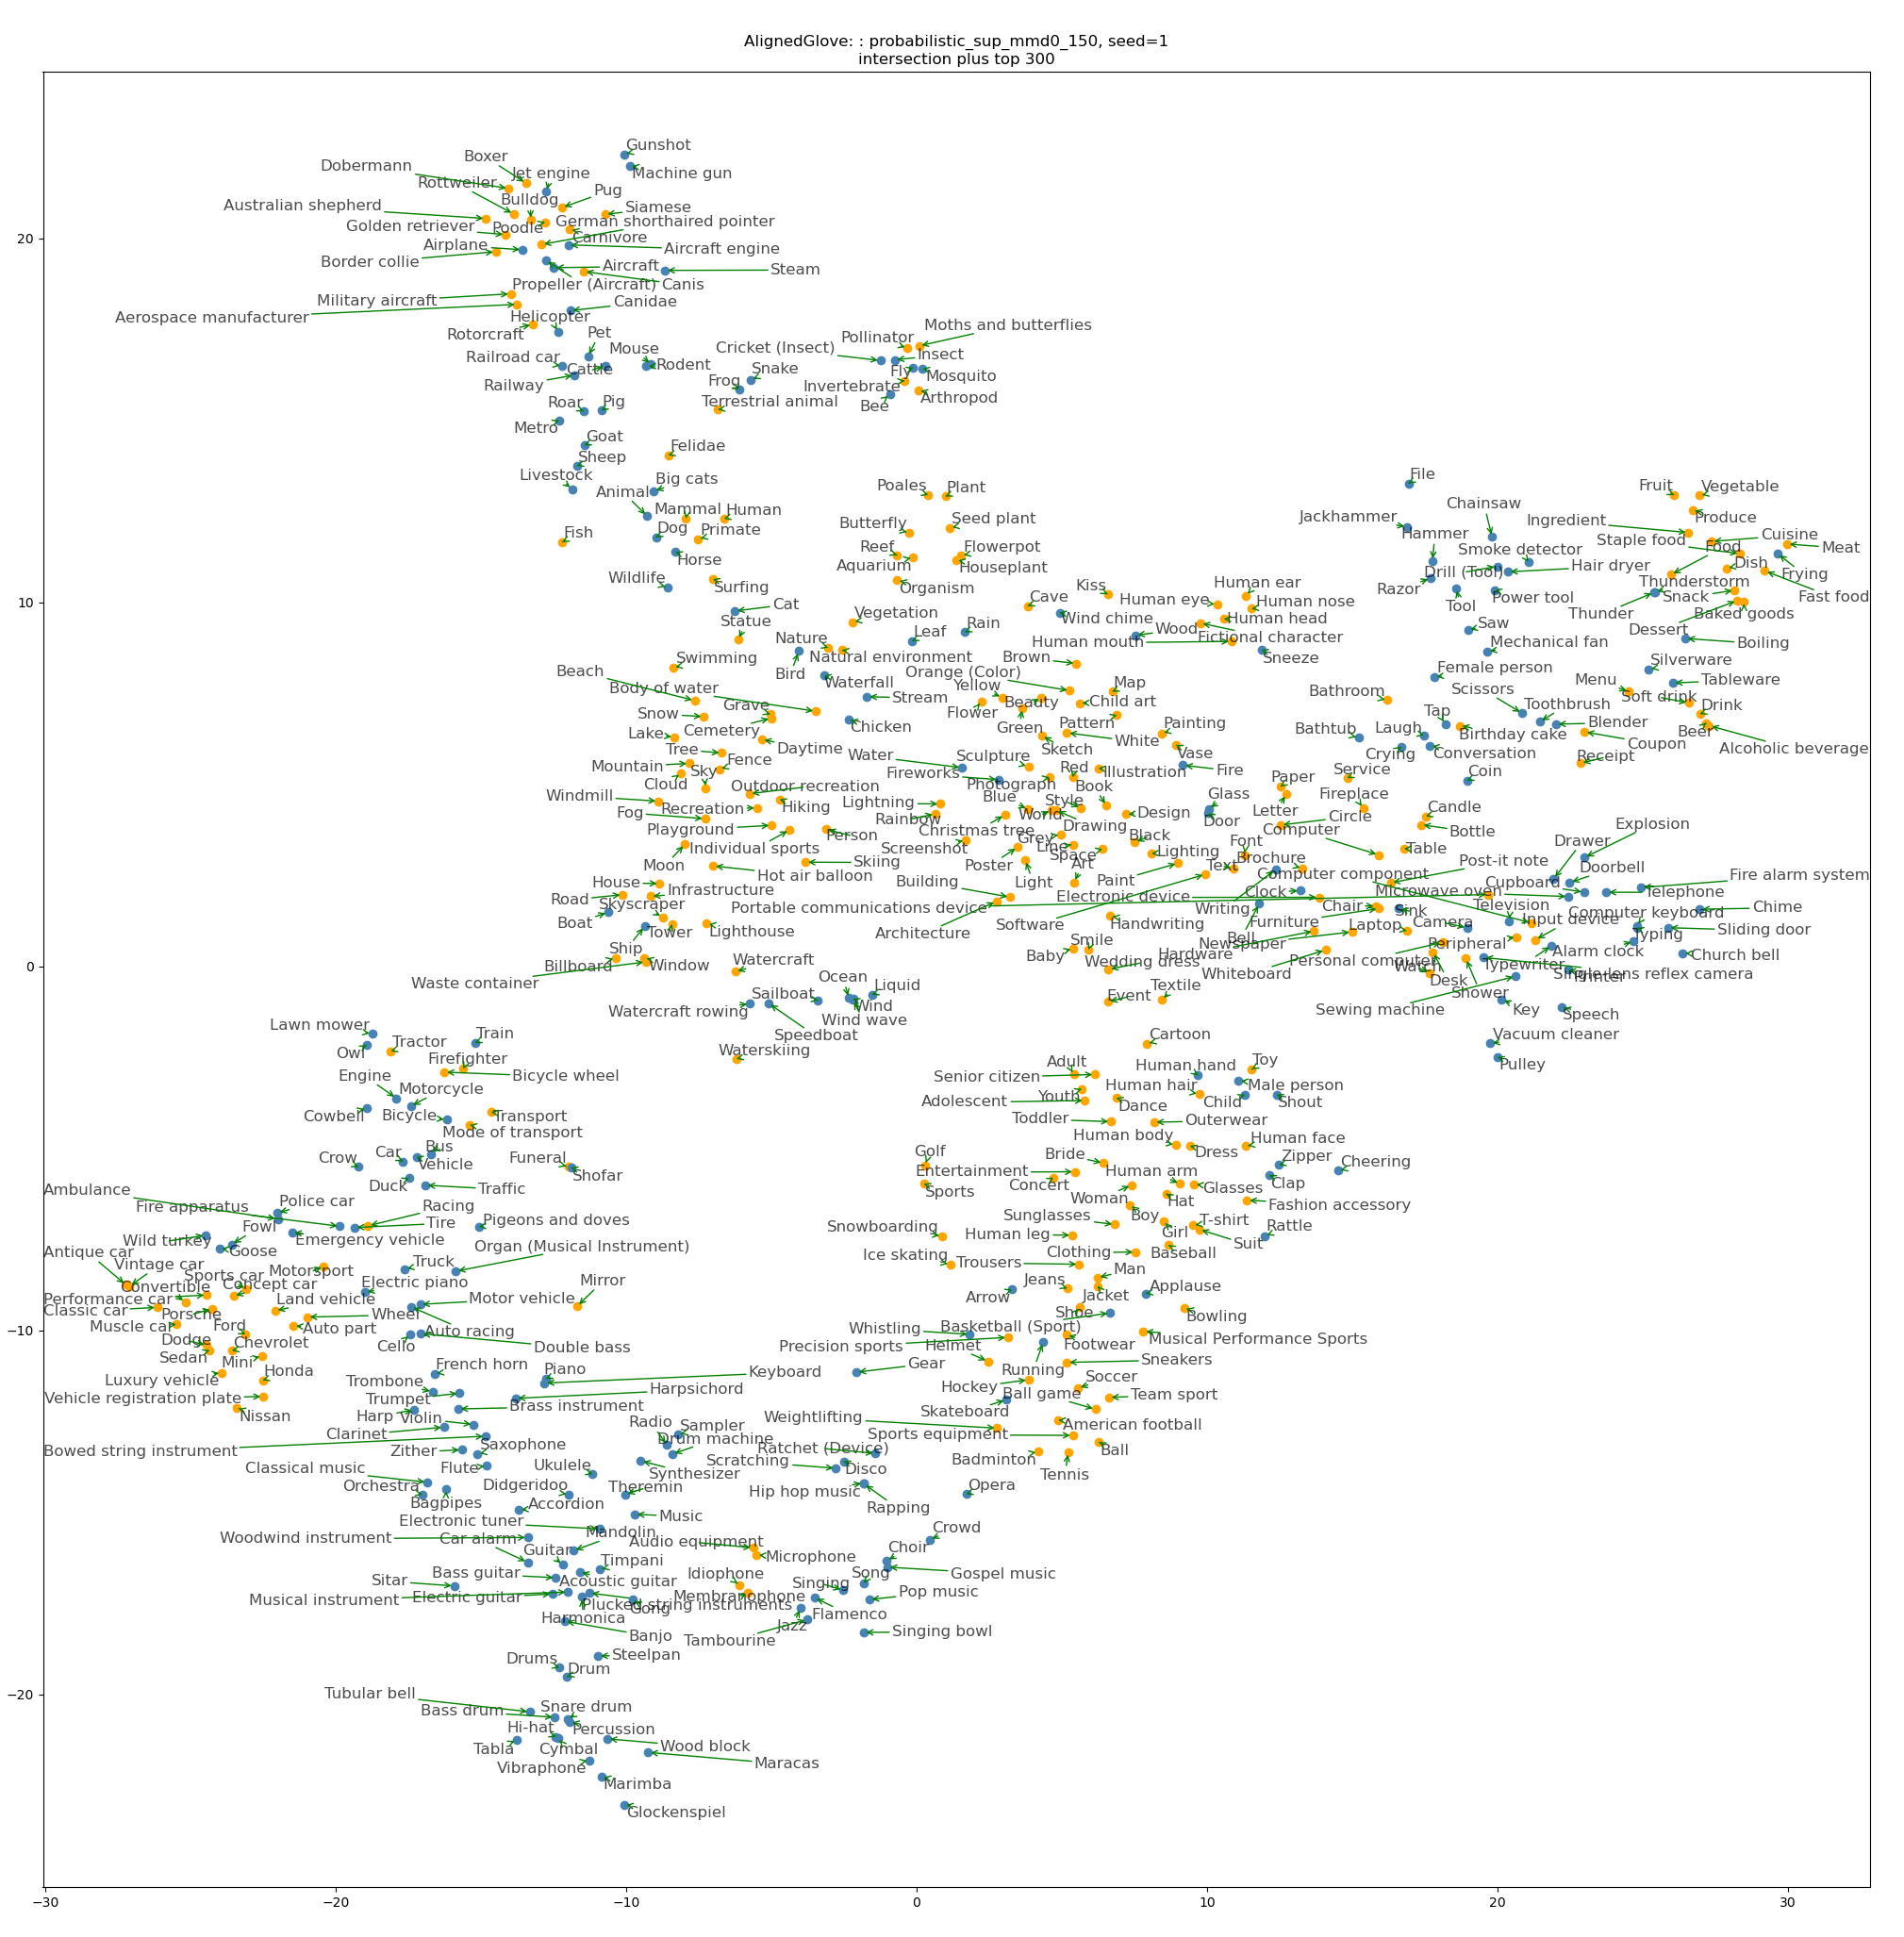
\includegraphics[width=\textwidth]{images/results/intersection_top300_tsne_openimages_probabilistic_sup_mmd0_150_AlignedGlove_1.png}
    \caption{
        \label{fig:openimagesaligned}
        t-SNE plot of concept embeddings for Open Images that are in the intersection of both domains (blue points) or in the top 300 most frequent (orange points). These are the embeddings for alignment run without MMD. See Figure \ref{fig:openimageszoom} for zoomed-in examples. 
    }
\end{figure}

\begin{figure}[H]
    \centering
    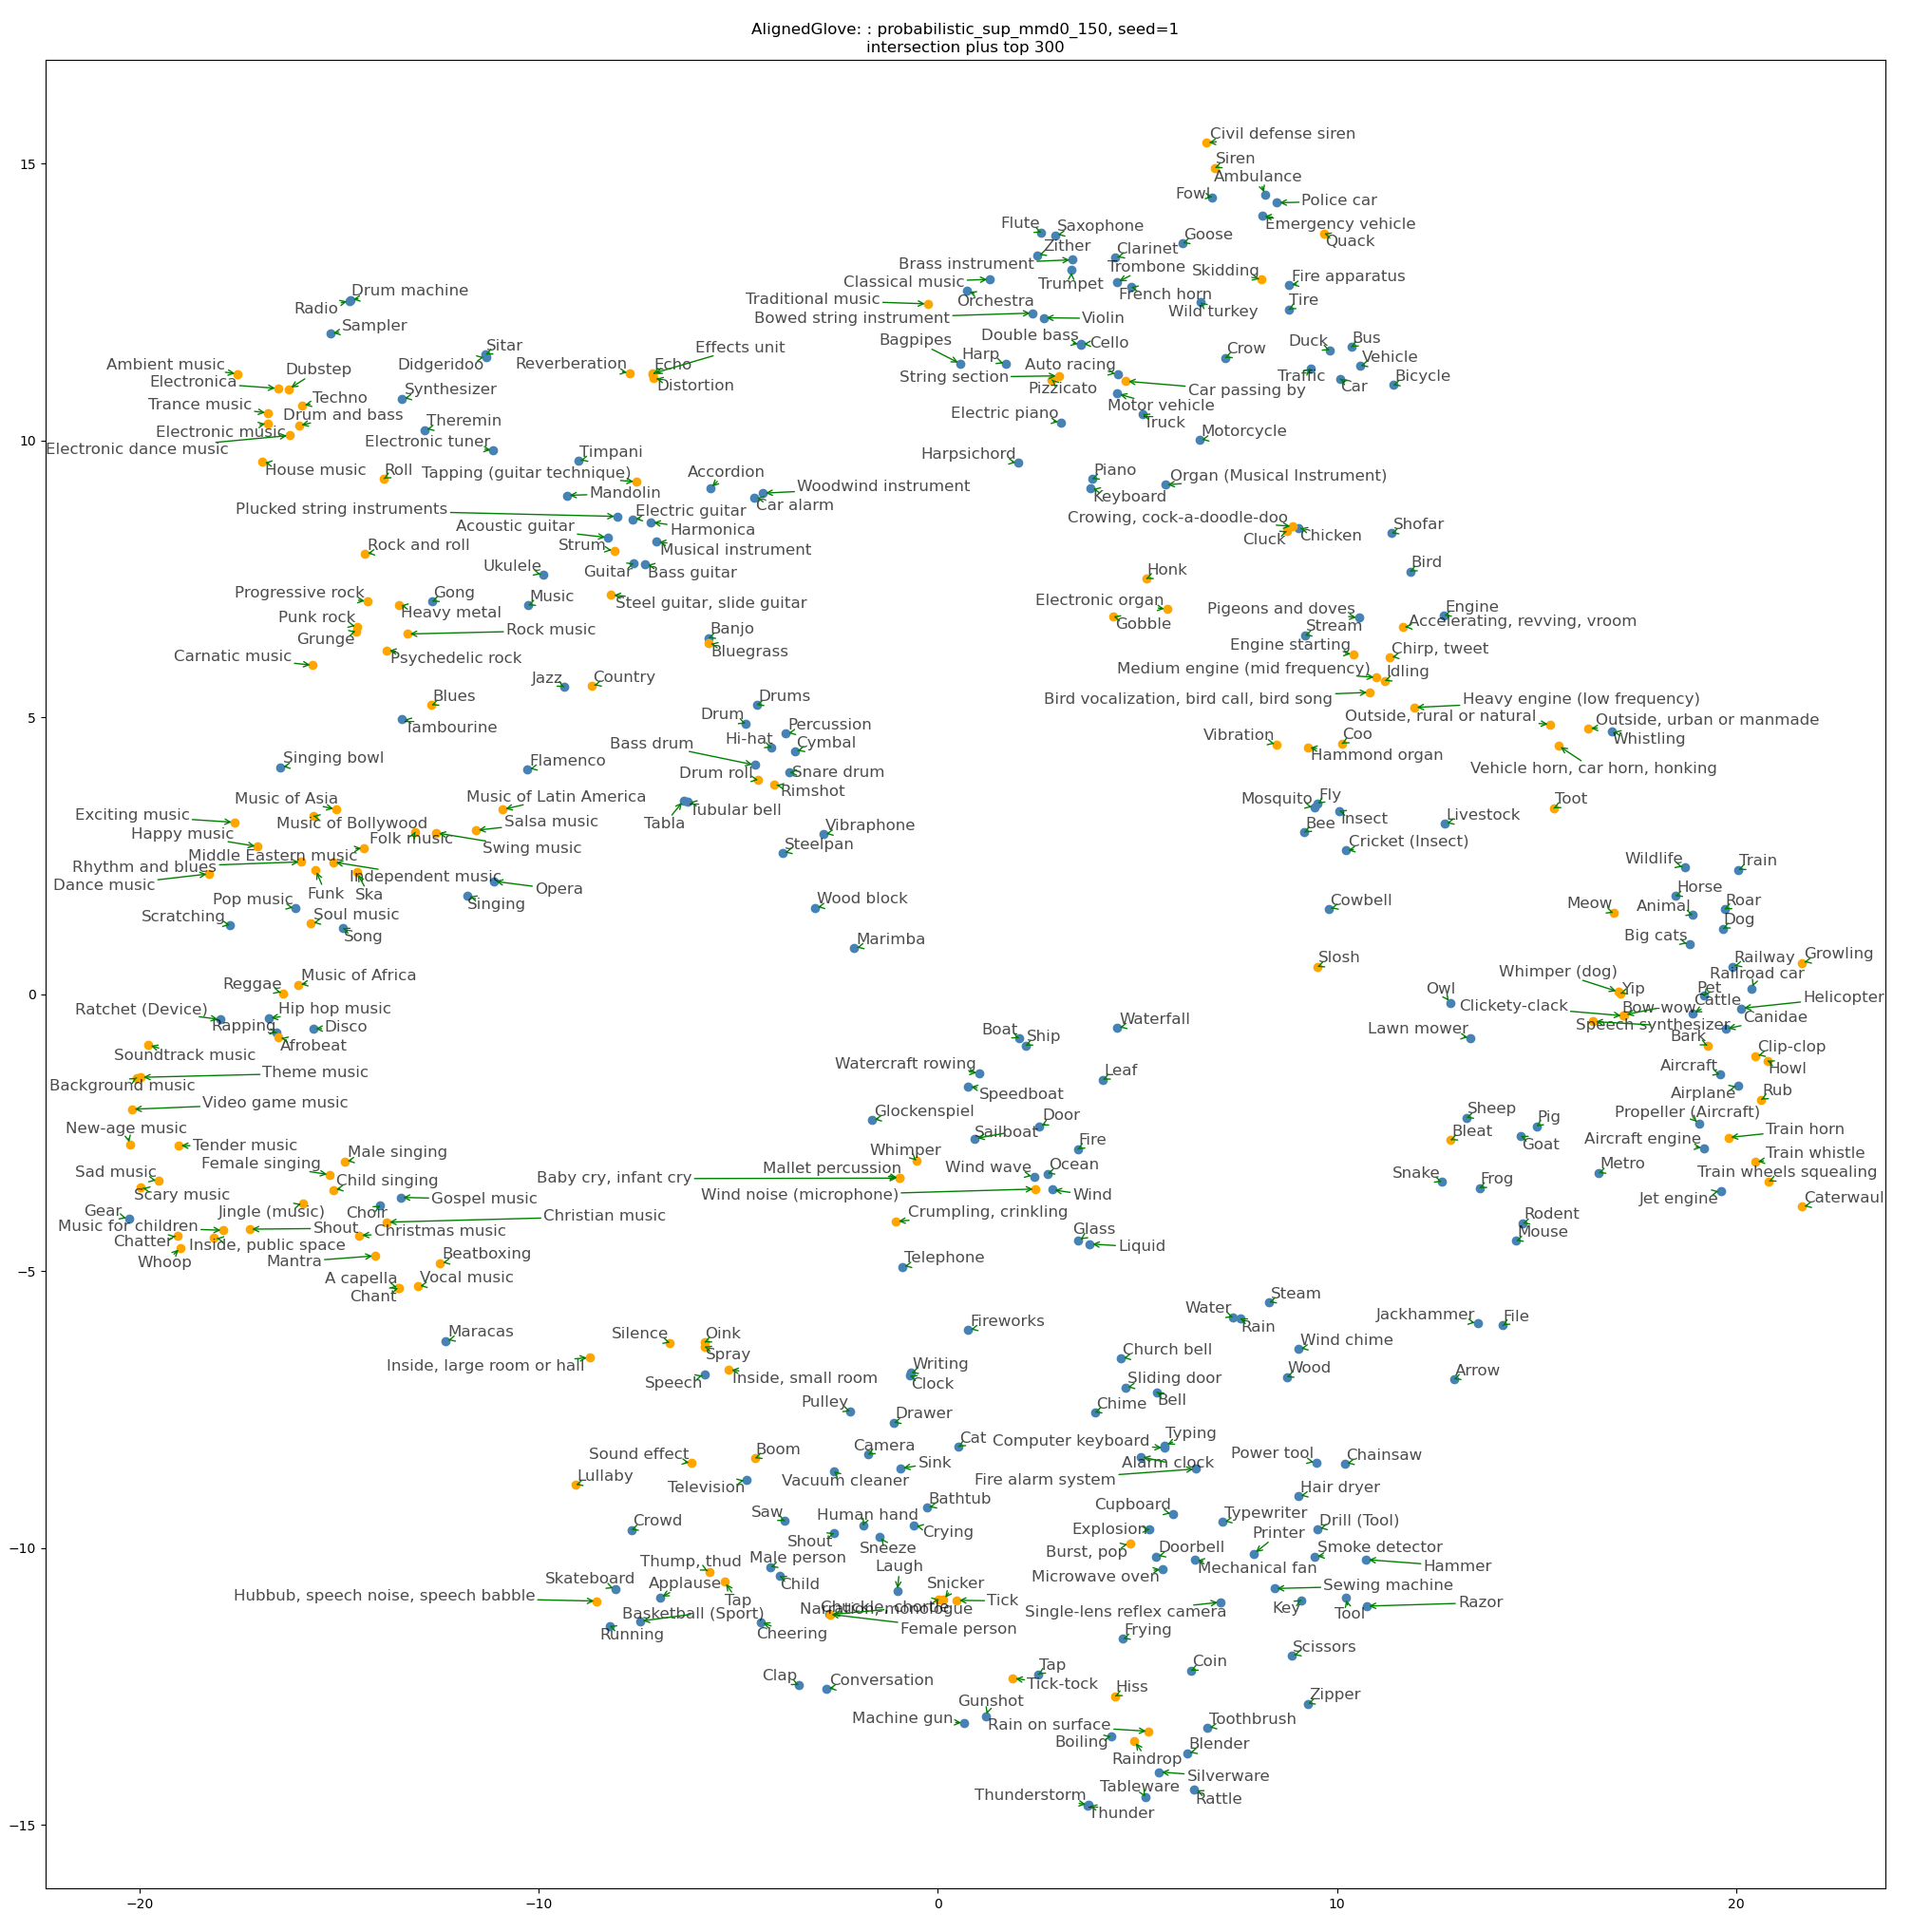
\includegraphics[width=\textwidth]{images/results/intersection_top300_tsne_audioset_probabilistic_sup_mmd0_150_AlignedGlove_1.png}
    \caption{
        \label{fig:audiosetaligned}
        t-SNE plot of concept embeddings for AudioSet that are in the intersection of both domains (blue points) or in the top 300 most frequent (orange points). These are the embeddings for alignment run without MMD. See Figure \ref{fig:audiosetzoom} for zoomed-in examples. 
    }
\end{figure}

In Figures \ref{fig:openimageszoom} and \ref{fig:audiosetzoom} below, we show some enlarged examples of clusters which show concepts in the intersection and out of the intersection. These clusters show that a good balance is struck between the GloVe loss and the distance loss / MMD; for an example of what happens when this balance is not found, see Figure \ref{fig:dysfunctional_clusters}, where the GloVe loss was not weighted sufficiently compared to the distance loss / MMD. 


\begin{figure}[H]

    \centering
    \fbox{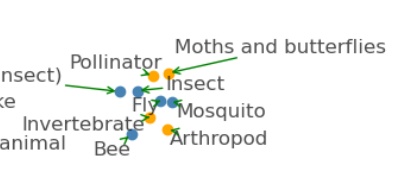
\includegraphics[width=0.4\textwidth]{images/results/openimages_zoom_insects.png}}
    \fbox{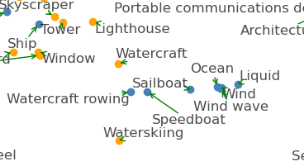
\includegraphics[width=0.4\textwidth]{images/results/openimages_zoom_ships.png}}
    \caption{\label{fig:openimageszoom}Enlarged view of two regions of the Open Images t-SNE plot, showing that concepts in and out of the intersection but semantically similar do form good clusters. As blue points denote concepts present in both domains and orange points denote concepts amongst the most frequent in the domain being examined, we want a mixture of orange and blue. }
\end{figure}

\begin{figure}[H]

    \centering
    \fbox{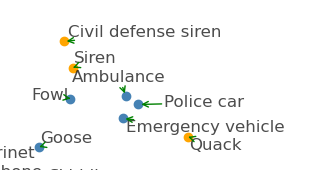
\includegraphics[width=0.4\textwidth]{images/results/audioset_zoom_sirens.png}}
    \fbox{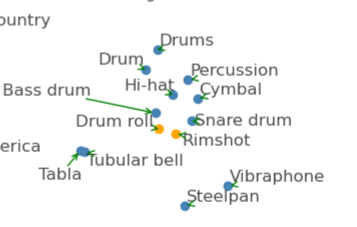
\includegraphics[width=0.4\textwidth]{images/results/audioset_zoom_drums.png}}
    \caption{\label{fig:audiosetzoom}Enlarged view of two regions of the AudioSet t-SNE plot showing the same phenomenon as described above.}
\end{figure}


\section{Statistics}

\subsection{Correlations}

We examine the correlations of self-similarity matrices over different random seeds, to get an idea of how consistent each set of embeddings is with itself. The similarity matrix of the embeddings for a given run is like a ``signature" of how the different concepts relate to each other within that run. We would like a high correlation of similarity matrices between runs, because that tells us that the algorithm is producing stable embeddings where concepts have the same degree of similarity with other concepts over many runs. 

\subsubsection{Average (Pearson) cross-correlation of self-similarity matrices of embedding means}

\begin{table}[H]
\centering
\begin{tabular}{lrrr}
\toprule
Domain &   Independent & Aligned     &  Aligned  \\
       &               & without MMD &  with MMD \\
\midrule
Open Images    & 0.590 $\pm$ 0.049 & 0.474 $\pm$ 0.044 &     0.420 $\pm$  0.040 \\
AudioSet    & 0.412 $\pm$ 0.045 &  0.399 $\pm$ 0.044  &      0.346  $\pm$ 0.043  \\
\bottomrule
\end{tabular}
\caption{\label{table:corrmeans}The similarity measure used for this table is the dot product of the means of the embeddings. The average is taken over all combinations of random seeds (1x2, 1x3, ..., 9x10).}
\end{table}

\subsubsection{Average (Pearson) cross-correlation of self-similarity matrices of samples of embeddings}
\begin{table}[H]
\centering
\begin{tabular}{lrrr}
\toprule
Domain &   Independent & Aligned     &  Aligned  \\
       &               & without MMD &  with MMD \\
\midrule
Open Images    & 0.589 $\pm$ 0.049 & 0.480 $\pm$ 0.040 &     0.434 $\pm$  0.040 \\
AudioSet    & 0.412 $\pm$ 0.044 &  0.399 $\pm$ 0.044  &      0.346  $\pm$ 0.043  \\
\bottomrule
\end{tabular}
\caption{\label{table:corrsamples}The similarity measure used for this table is mean of the dot product of 100 samples of each embedding (100 samples are taken, the pairwise dot product similarity computed, and the mean of those 100 similarity matrices is taken). This measure was used to take into account the variance of the embeddings, where the previous table used only the learned means of the embeddings. The average is taken over all combinations of random seeds (1x2, 1x3, ..., 9x10). It is not a typographical error that the values for AudioSet for mean of 100 similarity matrices are the same as the values for the embedding means in the previous table. }
\end{table}

The runs of the independently learned embeddings are more correlated with each other, compared to the equivalent calculation with the aligned embeddings. This means that the similarity matrices (of each run's embeddings with itself) are more consistent across runs. This correlation has dropped in the aligned runs, indicating that the output embeddings are less similar to themselves across runs. We can say that the alignment introduces more variation in the embeddings. MMD in particular seems to introduce more variability. 

\subsubsection{Mean Spearman correlation of entropy with frequency of occurrence}
\begin{table}[H]
\centering
\begin{tabular}{lrrr}
\toprule
Domain &   Independent & Aligned     &  Aligned  \\
       &               & without MMD &  with MMD \\
\midrule
Open Images    &  -0.179 $\pm$ 0.011 & 0.0421 $\pm$ 0.019 &     0.0362 $\pm$  0.012 \\
AudioSet    &  -0.400 $\pm$ 0.041 & -0.000539 $\pm$   0.074 &      0.0359  $\pm$ 0.026  \\
\bottomrule
\end{tabular}\\
\end{table}
There is a slight negative Spearman correlation between the entropy of a concept and its frequency of occurrence, in the independently learned cases. Entropies of less frequently occurring concepts are found to be higher, which is intuitively sensible; there is less information about those concepts so we would expect the variance, and therefore the entropy, to be higher. 

This correlation has largely disappeared in the aligned cases, being roughly around zero, indicating that there is now no relationship between the variance of the learned embedding for a concept and the frequency of that concept in the dataset. In this respect, the aligned probabilistic embeddings are less informative than the independent probabilistic ones. 
\subsection{Entropy plots of aligned embeddings}

\todo[inline]{I think the absolute positions of the entropy distributions for each run are not significant eg. comparing independent / aligned / aligned + MMD for seed = 1 is not relevant. I think it is the comparison of the distributions across all runs that is significant eg. independent for all seeds, aligned for all seeds, etc. }

\subsubsection{Open Images}

\begin{figure}[H]
\label{fig:entropyviolinimgs}
\centering
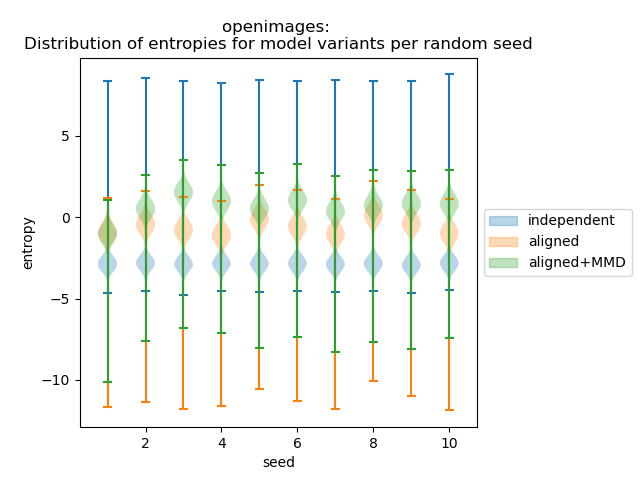
\includegraphics[width=\textwidth]{images/results/openimages_entropies_violin.png}
\caption{Violin plots of entropy distributions for independent embeddings, aligned without MMD and aligned with MMD. The entropy distribution for aligned embeddings is more variable between runs than that for independent embeddings. The use of MMD increases this variability. These results are consistent with the self-similarity correlations between runs shown in Tables \ref{table:corrmeans} and \ref{table:corrsamples}, which also indicated that the aligned embeddings were more unstable over different runs.}
\end{figure}

\subsubsection{AudioSet}

\todo[inline]{Does it mean anything that the aligned entropies are all lower in value (more negative) than aligned + MMD and independent? See above note on the relative comparisons per seed}

\begin{figure}[H]
\label{fig:entropyviolinaudio}
\centering
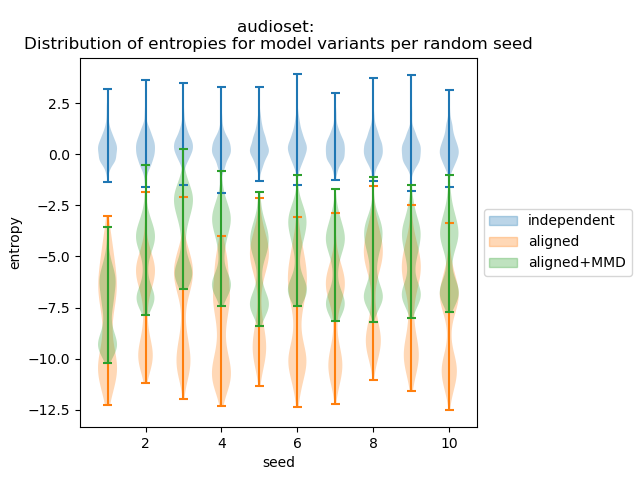
\includegraphics[width=\textwidth]{images/results/audioset_entropies_violin.png}
\caption{Violin plots of entropy distributions for independent embeddings, aligned without MMD and aligned with MMD. The aligned embeddings, whether run with or without MMD, show a bimodal entropy distribution and much greater variability than that of the independent embeddings.  These results are consistent with the self-similarity correlations between runs shown in Tables \ref{table:corrmeans} and \ref{table:corrsamples}, which also indicated that the aligned embeddings were more unstable over different runs. }
\end{figure}

\section{Alignment accuracy and embedding quality}

The table below shows the alignment accuracy for both domains, over 10 random seeds. Using the MMD statistic as a component of the loss marginally increased the accuracy. 

\begin{table}[H]
\centering
\begin{tabular}{lrrrr}
  \toprule
       &    Open Images&               &  AudioSet    &            \\
{Seed} &    Without MMD &   With MMD   &  Without MMD &   With MMD \\
\midrule
1    &       0.9479 &        0.9478&    0.9478 &  0.9652  \\
2    &       0.9565 &        0.9826&    0.9696 &  0.9826  \\
3    &       0.9348 &        0.9565&    0.9565 &  0.9783  \\
4    &       0.9522 &        0.9652&    0.9565 &  0.9565  \\
5    &       0.9478 &        0.9609&    0.9435 &  0.9696  \\
6    &       0.9522 &        0.9739&    0.9739 &  0.9696  \\
7    &       0.9652 &        0.9652&    0.9478 &  0.9739  \\
8    &       0.9696 &        0.9522&    0.9609 &  0.9522  \\
9    &       0.9565 &        0.9565&    0.9609 &  0.9783  \\
10   &       0.9609 &        0.9522&    0.9652 &  0.9783  \\
\midrule                                                         
mean &       0.9543 &        0.9613 &   0.9583 &  0.9704  \\
\bottomrule
\end{tabular}
\end{table}

High alignment accuracy between embeddings in both domains does not necessarily mean the embeddings are good. Figure \ref{fig:dysfunctional_clusters} below is a t-SNE plot of aligned embeddings (reduced to 2 dimensions) of very high accuracy (97\%), meaning that the embeddings in Open Images and AudioSet are well aligned. However, the actual embeddings did not form good clusters; concepts that were related semantically tended not to be close in embedding space. 

\begin{figure}[H]

    \centering
    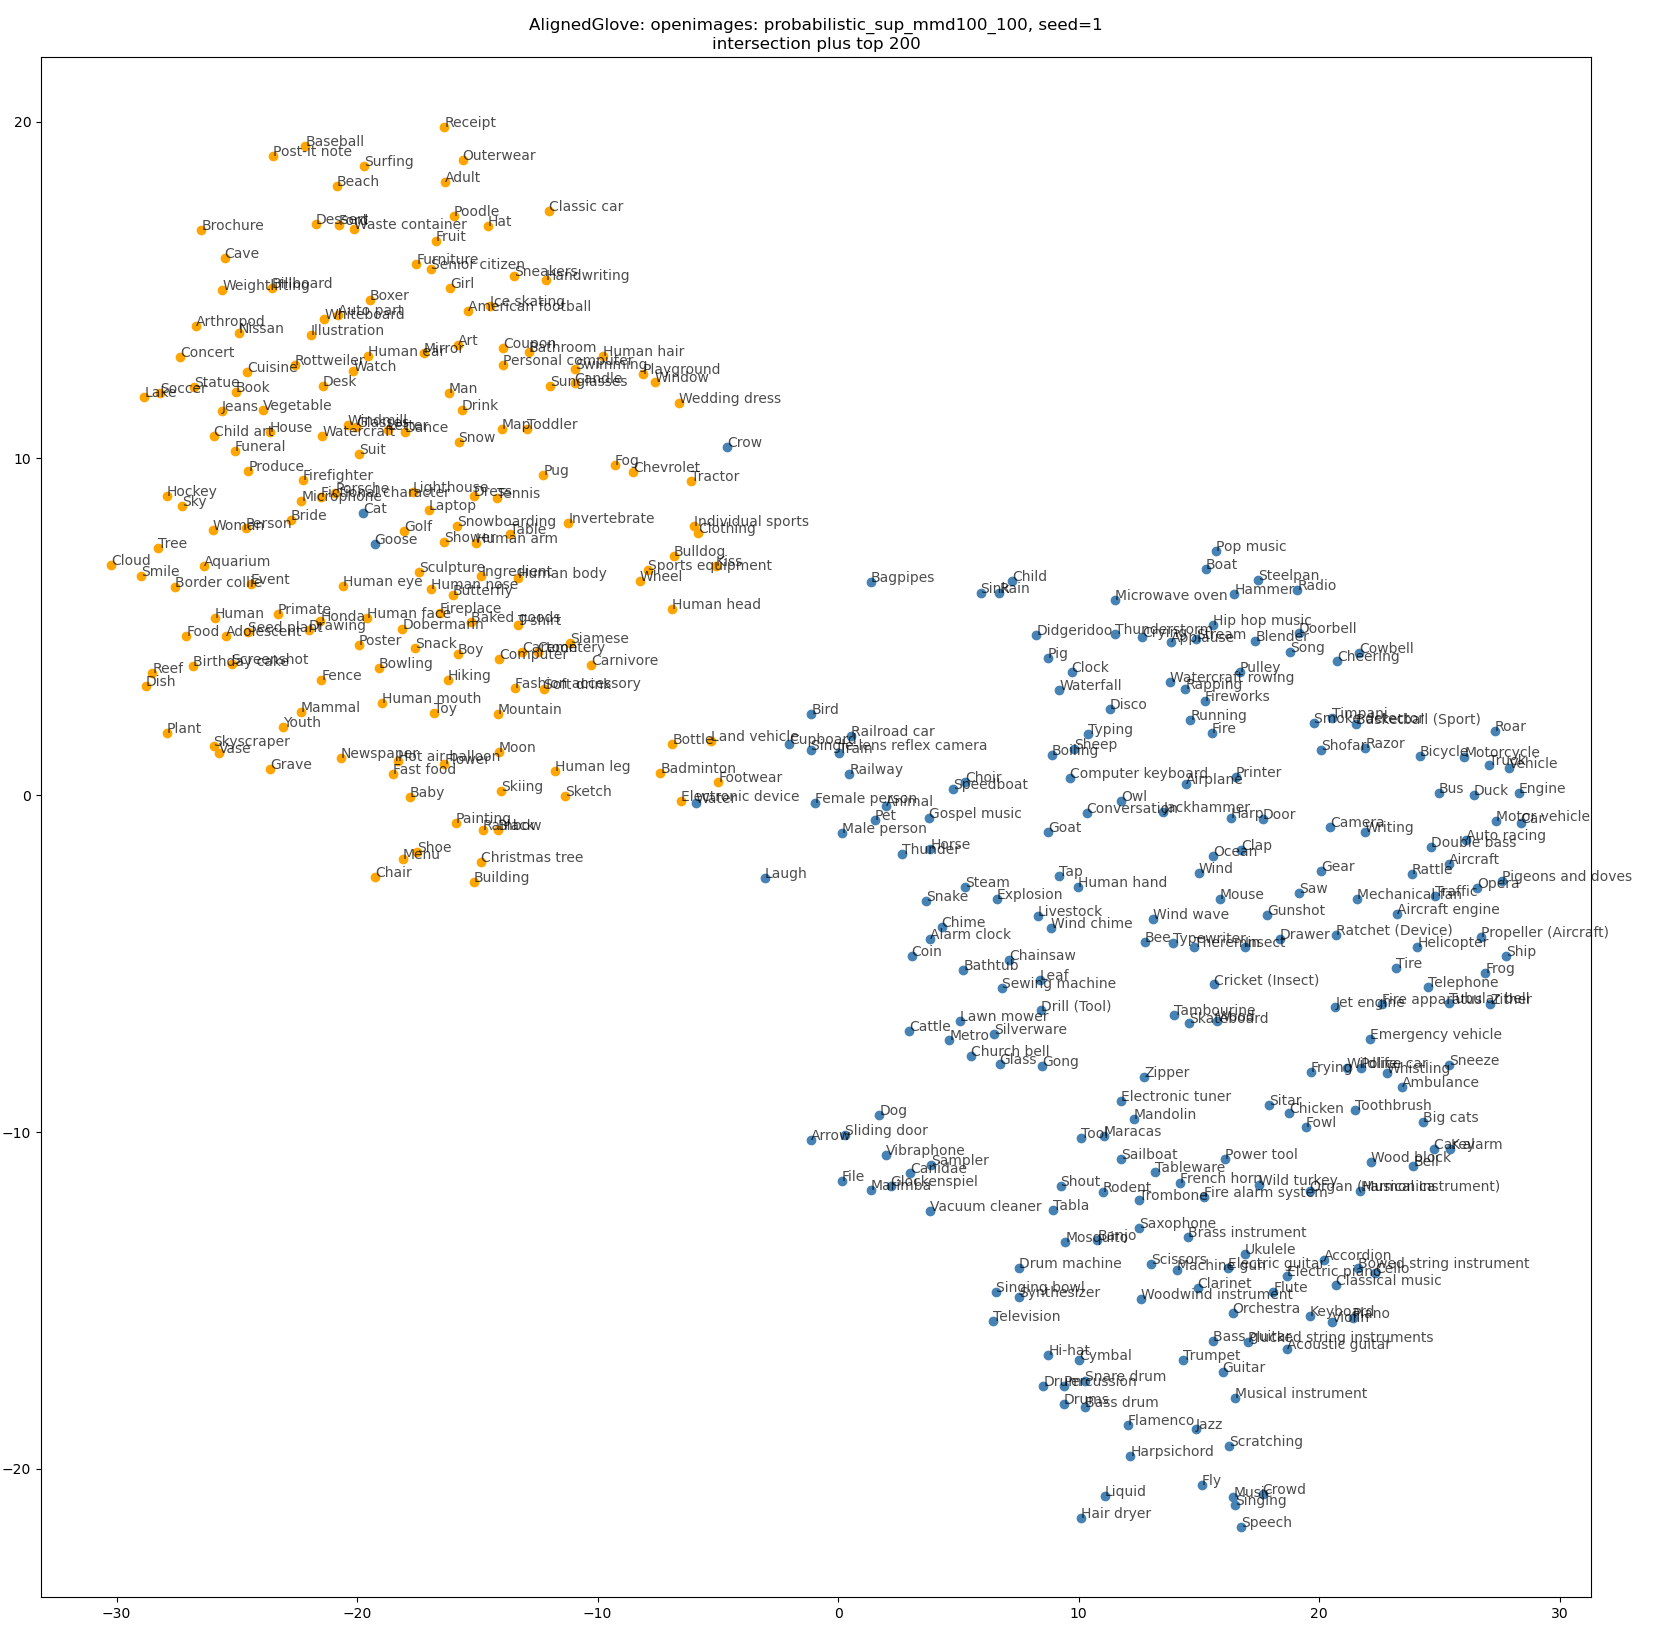
\includegraphics[width=1.0\textwidth]{images/method/probabilistic_aligned/dysfunctional_clusters.png}
    \caption{\label{fig:dysfunctional_clusters}
        The alignment accuracy for this set of embeddings is 97\%. The blue points denote concepts that are in the intersection of concepts (present in both Open Images and AudioSet). The orange points denote concepts that are in the 200 most frequent concepts occurring in Open Images. It is immediately visible that the algorithm has clustered concepts in the intersection degenerately; concepts that are in the intersection are more likely to be close to other concepts in the intersection rather than concepts that are semantically close.
    }
\end{figure}

Hence, alignment accuracy is insufficient as a metric. We can also examine the average Pearson correlations of the similarity matrices of the aligned and independent embeddings over 10 random seeds, for the two model variants: 

%inspect_results.py function aligned_vs_ind_corrs
\begin{table}[H]
\centering
\begin{tabular}{lrrrr}
  \toprule
       &    Open Images&               &  AudioSet    &            \\
{} &    Without MMD &   With MMD   &  Without MMD &   With MMD \\
\midrule
   &       0.532 \pm 0.035 &   0.465 \pm 0.038 &   0.334 \pm 0.036 &  0.331 \pm 0.038  \\
\bottomrule
\end{tabular}
\end{table}

The above are aggregate statistics that only tell us that there is a positive correlation between the similarities of the aligned and independent embeddings. We do not know if the aligned embeddings are actually semantically more meaningful than the independent, or the other way around. 

\subsection{Comparing aligned embeddings with human similarity scores}

A plausible measure of embedding quality would be a comparison of the similarity of concept pairs as calculated from embeddings, with the similarity of concept pairs as evaluated by humans. In order to do this, we need to find datasets that capture human ratings of similarity. If our alignment algorithm is good, we should expect that the aligned embeddings are of higher quality than the independently learned embeddings and correlate more highly with human similarity judgement. 

\textbf{MTURK-771}: The MTURK-771 dataset was created by the authors of \cite{mturk771}, a study in learning the relatedness of word pairs. The predictions are tested by comparing the Spearman correlation of its predictions with human judgements. The MTURK-771 dataset comprises 771 pairs of words with human-rated similarity scores, collected using the Amazon Mechanical Turk tool. The intersection of the 771 word pairs with our Open Images and AudioSet concepts was small - 171 (0.013\%)  for Open Images and only 3 (0.0071\%) for AudioSet. 

\textbf{WordNet}: The WordNet \cite{WordNet} lexical database contains English nouns, verbs and adjectives grouped according to synonymy (semantic similarity) and hypernymy/hyponymy (hierarchy). Words are represented by ``synsets" which denote a particular sense of the word (for example, ``orange" may refer to the colour or the fruit). Therefore, one word may map to several synsets. The relationships between word senses were hand-encoded from various corpora and thesauri, which themselves were human-curated; therefore, we consider the lexical and semantic information contained within WordNet to be an appropriate representation of human judgement. The WordNet database can be accessed directly from the \texttt{nltk} Python package. 

There is a substantial overlap between pairs of words found in WordNet and pairs of concepts from our dataset.  Out of approximately 128 million (128005400) nonzero pairs occurring in Open Images, approximately 27 million (27052350, 21.1\%) are also present in WordNet. Out of 42002 nonzero pairs in AudioSet, 19208 (45.7\%) are also present in WordNet. 

\textbf{ILSVRC}: A third available dataset originates from a prototype model for \cite{RoadsLoveCVPR}, in which human similarity judgements of pairs of concepts were collected to supplement the ImageNet Large-Scale Visual Recognition Challenge (ILSVRC) 2012 task. This dataset will be referred to as the ``enhanced ILSVRC" dataset. These judgements were collected from participants using Amazon Mechanical Turk. The data collection process used probabilistic techniques for trial selection to maximise the expected information gain from each trial. In this dataset, 147070 (0.115\%) pairs overlap with Open Images, and 93 (0.221\%) pairs overlap with AudioSet. One word, ``tick", was removed from the AudioSet pairs when computing the comparison, because that label as used in AudioSet is used to describe the sound and not the insect. We know that the ImageNet label corresponds to the insect. 

We adopt the method used by \cite{mturk771} of comparing the Spearman correlation of the similarity of our embedding concept pairs with the similarity of the human-measured dataset to evaluate the quality of aligned embeddings compared to independently learned embeddings. The Spearman correlation is used because we wish to evaluate whether there is a monotonic relationship, and the similarity measures all use different scales. The cosine similarity measure is used as it contains the dot product, which is an input into the GloVe algorithm that generates the embeddings, and the magnitude of the embeddings is not meaningful. 

The similarity of two concepts with indexes $i$ and $j$ in embedding space is:

\begin{equation*}
s_{ij} = \frac{\vece_i \cdot \vece_j}{||\vece_i||_2 \medspace ||\vece_j||_2}
\end{equation*}

where $\vece_i$ represents the $i$-th embedding.

If the correlation with the human similarity dataset is higher for aligned embeddings than for independently learned embeddings, this indicates that the alignment process is adding value, resulting in more cognitively plausible embeddings. This is because it indicates that the aligned embedding pairs are in aggregate more like human judgement of similarity than the independent embedding pairs. We will use this as a metric for embedding quality, where higher quality means more similar to human judgement.  We evaluate the model variants with and without MMD by this metric to assess the effect of MMD. 

The MTURK-771 and enhanced ILSVRC datasets are pre-existing mappings of concept pairs to similarity values, which can be used without any preprocessing. There is no such WordNet dataset of direct similarity, so we have to construct one. WordNet makes available similarity measures between synsets that can be computed directly from the Python library. We choose the Leacock-Chodorow (LCH) similarity measure \cite{LeacockChodorow}, which takes the shortest path between the two synsets, scaled by the maximum depth from the top of the taxonomy tree of the two synsets (this measure was chosen as it is the only one that combines path length between nodes and depth of the tree).  

As a single word or phrase may map to several synsets, and we have no sense information in our Open Images / AudioSet concept names to disambiguate between choices, we may have more than one feasible synset pair per concept pair in our dataset. We use the following heuristic algorithm to decide which specific synset pair's scores to use:

\begin{itemize}
    \item Check every pair in the domain (Open Images or AudioSet) that appears at least once (its entry in the co-occurrence matrix is nonzero).
    \item Convert the pair words to lowercase with spaces replaced with underscores (this is the WordNet naming scheme).
    \item Check if both words have synsets in WordNet. If either does not, ignore the pair.
    \item For each combination of the first 2 synsets for each word (up to 4 pairs in total), compute the LCH similarity if both elements in the pair have the same part of speech, otherwise ignore the pair. \footnote{WordNet similarity is not defined for synsets which do not have the same parts of speech. } This is to handle pairs like ``mandarin orange" and ``orange". ``Mandarin orange" has two synsets; the first refers to the mandarin orange tree, and the second refers to the fruit. Therefore the second ``mandarin orange" synset matches the first ``orange" synset (which denotes the fruit, rather than the colour) more closely. One mode of failure for this algorithm is for words that occur in both Open Images and AudioSet but with different meanings, for example, ``tap" and ``tick" are different concepts when referring to objects or sounds. 
    \item The WordNet similarity for the pair is taken to be the largest such value. This algorithm will therefore be biased high.
\end{itemize}


\subsection{Results of comparison with human similarity metrics}

\subsubsection{Degree of overlap of human similarity datasets with domain pairs}

These are the percentages of data overlap for the different domains:

\begin{table}[H]
\centering
\begin{tabular}{lrr}
\toprule
{Human similarity dataset} &  Open Images &   AudioSet\\
\midrule
MTURK-771    &     0.013\% &  0.0071\%  \\
WordNet    &     21.1\% &  45.7\%  \\
enhanced ILSVRC    &    0.115\% &  0.221\% \\
\bottomrule
\end{tabular}
\centering
\end{table}

\subsubsection{Open Images, Spearman correlation with human similarity metrics}
\begin{table}[H]
\centering
\begin{tabular}{lrrrrrrrrr}
  \toprule
   &     &   MTURK-771        &               &      &    WordNet       &               &     &  ILSVRC           & \\
{Seed} &  Ind. &   Aligned &  Aligned  & Ind. &   Aligned &  Aligned  & Ind. &   Aligned &  Aligned   \\
{}     &              &           & +MMD      &            &            & +MMD      &             &           &   +MMD \\
\midrule
1    &     0.357 &  0.306 &   0.331 &     0.205 &  0.229 &    0.228 &   0.524 &  0.493 &  0.488  \\
2    &     0.343 &  0.271 &   0.296 &     0.196 &  0.221 &    0.230 &   0.471 &  0.460 &  0.458  \\
3    &     0.376 &  0.338 &   0.287 &     0.200 &  0.240 &    0.240 &   0.483 &  0.486 &  0.433  \\
4    &     0.343 &  0.300 &   0.290 &     0.210 &  0.233 &    0.229 &   0.514 &  0.531 &  0.482 \\
5    &     0.358 &  0.256 &   0.225 &     0.191 &  0.226 &    0.226 &   0.505 &  0.466 &  0.456  \\
6    &     0.374 &  0.309 &   0.271 &     0.207 &  0.239 &    0.237 &   0.541 &  0.473 &  0.451  \\
7    &     0.347 &  0.297 &   0.292 &     0.208 &  0.229 &    0.239 &   0.506 &  0.468 &  0.447  \\
8    &     0.343 &  0.284 &   0.283 &     0.215 &  0.217 &    0.218 &   0.553 &  0.458 &  0.468  \\
9    &     0.340 &  0.279 &   0.271 &     0.217 &  0.224 &    0.233 &   0.508 &  0.463 &  0.439  \\
10   &     0.367 &  0.267 &   0.284 &     0.207 &  0.225 &    0.230 &   0.531 &  0.464 &  0.452  \\
\midrule                                                                                         
mean &     0.355 &  0.291 &   0.283 &     0.205 &  0.228 &    0.231 &   0.514 &  0.476 &  0.458  \\
\bottomrule
\end{tabular}
\end{table}

\subsubsection{Open Images, differences of Spearman correlation between aligned model variant and independently learned embeddings}


\begin{table}[H]
\centering
\begin{tabular}{lrrrrrr}
  \toprule
       &   MTURK-771 &           &  WordNet  &           &  ILSVRC  &            \\
{Seed} &   Aligned   &  Aligned  &   Aligned &  Aligned  &  Aligned &  Aligned   \\
{}     &             & +MMD      &            & +MMD     &          &   +MMD     \\
\midrule
1    &     -0.0512 &    -0.0260  &   0.0244 &     0.0234 &    -0.0305 &    -0.0353   \\
2    &     -0.0716 &    -0.0465  &   0.0255 &     0.0346 &    -0.0107 &    -0.0130   \\
3    &     -0.0374 &    -0.0884  &   0.0402 &     0.0402 &     0.00349 &    -0.0495   \\
4    &     -0.0433 &    -0.0530  &   0.0232 &     0.0185 &     0.0174 &    -0.0322   \\
5    &     -0.102  &    -0.133   &   0.0354 &     0.0356 &    -0.0385 &    -0.0484   \\
6    &     -0.0650 &    -0.103   &   0.0320 &     0.0301 &    -0.0686 &    -0.0904   \\
7    &     -0.0509 &    -0.0552  &   0.0216 &     0.0308 &    -0.0383 &    -0.0595   \\
8    &     -0.0592 &    -0.0599  &   0.00189 &    0.00313 &   -0.0948 &    -0.0851   \\
9    &     -0.0614 &    -0.0686  &   0.00696 &    0.0166 &    -0.0448 &    -0.0691   \\
10   &     -0.0995 &    -0.0828  &   0.0184 &     0.0235 &    -0.0674 &    -0.0793   \\
\midrule                                                                                          
mean &     -0.0641 &    -0.0716  &   0.0230 &     0.0256 &    -0.0373 &    -0.0562   \\
\bottomrule
\end{tabular}
\end{table}


For Open Images, using the WordNet comparison metric, the aligned embeddings are more correlated with human similarity than the independently learned embeddings, as the mean Spearman correlation of alignment pairwise cosine similarity with WordNet similarity is greater for aligned embeddings than for independent embeddings. 

The reverse is observed with the MTURK-771 comparison metric, but we do note that this is a very small dataset of only 170 pairs present in both Open Images (out of 120 million pairs) and MTURK-771. The same phenomenon as with MTURK-771 is also observed when comparing with the ILSVRC metric, where the aligned embeddings are less correlated with human judgement than the independently learned embeddings degree of correlation with human judgement. 

However, the ILSVRC dataset is unbalanced, and some of the choices of included concepts are strange. There are 1000 concepts present in it, of which 124 are different breeds of dog. In fact, 398 of the concepts present in the ILSVRC are different types of animal. There are some concepts in the selected 1000 that almost certainly are not amongst the most common humanly known concepts, for example, ``shoji"\footnote{A Japanese sliding door made of paper.} and ``bicycle-built-for-two" (with ``bicycle" not present). The only flowers present are ``cardoon" \footnote{A type of thistle.}, ``daisy" and ``yellow lady's slipper". In short, the concepts represented in the ILSVRC dataset do not appear to be a very good sample of human concepts. To investigate whether the imbalance of the dataset was affecting results, runs were tried of the ILSVRC dataset excluding all the animals and then only including animals, but the results were broadly the same. 

\textbf{Given that the overlap of WordNet pairs with our domain pairs is considerable (21.1\% for Open Images and 45.7\% for AudioSet), we think that the higher correlation with WordNet similarity for aligned Open Images embeddings constitutes evidence that embedding quality is improved by alignment.} This would be consistent with hypotheses that multi-task learning adds value by producing a model that generalises better.

However, playing devil's advocate, we do also point out that the WordNet similarity score is an artificial score inferred from properties of the WordNet database, whereas the MTURK-771 and  ILSVRC similarity measures are directly collected from humans. 

Using the MMD as a component of the loss appears to increase accuracy, as well as alignment quality as measured against the WordNet metric. If comparing to the MTURK-771 and ILSVRC datasets, using MMD appears to decrease the alignment quality.  

\subsubsection{AudioSet, Spearman correlation with human similarity metrics}

MTURK-771 is excluded from this comparison, as with only 3 pairs present in both MTURK-771 and AudioSet, no meaningful results could be obtained. 

\begin{table}[H]
\centering
\begin{tabular}{lrrrrrrrrr}
  \toprule
       &       &   WordNet &           &      &  ILSVRC   &            \\
{Seed} &  Ind. &   Aligned &  Aligned  & Ind. &   Aligned &  Aligned   \\
{}     &       &           & +MMD      &      &           &   +MMD     \\
\midrule
1    &    0.139 &  0.163 &   0.153 &   0.635 &  0.683 &   0.502 &   \\
2    &    0.132 &  0.130 &   0.147 &   0.585 &  0.687 &   0.651 &  \\
3    &    0.157 &  0.175 &   0.133 &   0.647 &  0.428 &   0.617 &  \\
4    &    0.147 &  0.148 &   0.169 &   0.560 &  0.610 &   0.649 &  \\
5    &    0.116 &  0.151 &   0.152 &   0.562 &  0.513 &   0.578 &  \\
6    &    0.144 &  0.134 &   0.125 &   0.631 &  0.609 &   0.504 &  \\
7    &    0.150 &  0.134 &   0.170 &   0.539 &  0.563 &   0.546 &  \\
8    &    0.140 &  0.183 &   0.128 &   0.553 &  0.675 &   0.682 &  \\
9    &    0.147 &  0.136 &   0.187 &   0.524 &  0.718 &   0.681 &  \\
10   &    0.150 &  0.166 &   0.143 &   0.607 &  0.717 &   0.699 &  \\
\midrule                                                                   
mean &    0.142 &  0.152 &   0.151 &   0.584 &  0.620 &   0.611 &  \\
\bottomrule
\end{tabular}
\end{table}



\subsubsection{AudioSet, differences of Spearman correlation between aligned model variant and independently learned embeddings}


\begin{table}[H]
\centering
\begin{tabular}{lrrrr}
  \toprule
       &     WordNet  &           &  ILSVRC  &            \\
{Seed} &      Aligned &  Aligned  &  Aligned &  Aligned   \\
{}     &               & +MMD     &          &   +MMD     \\
\midrule
1    &    0.0237 &     0.0138  &   0.0489 &    -0.132    \\
2    &   -0.00278 &     0.0144 &   0.102  &     0.0662   \\
3    &    0.0176 &    -0.0237  &  -0.219  &    -0.0293   \\
4    &    0.00162 &     0.0221 &   0.0497 &     0.0886   \\
5    &    0.0350 &     0.0361  &  -0.0488 &     0.0160   \\
6    &   -0.00988 &    -0.0189 &  -0.0218 &    -0.127    \\
7    &   -0.0156 &     0.0202  &   0.0237 &     0.00677  \\
8    &    0.0423 &    -0.0127  &   0.122  &     0.129    \\
9    &   -0.0117 &     0.0401  &   0.194  &     0.157    \\
10   &    0.0160 &    -0.00696 &   0.110  &     0.0918   \\
\midrule                                                                    
mean &    0.00964 &     0.00844 &   0.0361 &     0.0267  \\
\bottomrule
\end{tabular}
\end{table}

\textbf{When compared with both WordNet and ILSVRC, AudioSet aligned embeddings are more correlated with human similarity judgement than the independently learned embeddings.}  However, only 93 pairs present in AudioSet overlap with ILSVRC pairs, so this is not a large sample for comparison. It is also subject to the vagaries of the ILSVRC dataset concept choice, as discussed in the previous section. We observe an asymmetry, where Open Images improves AudioSet with respect to ILSVRC, but AudioSet does not improve Open Images, which could be due to the fact that there are nearly 40 times as many concepts in Open Images than AudioSet, so there is simply much more information there to assist with alignment of AudioSet than there is in the other direction. 

Similar to Open Images, including MMD in the loss function increases accuracy, but it slightly decreases alignment quality when compared to independently learned embeddings using both WordNet and ILSVRC metrics.

\subsection{Overall results}
\textbf{When compared with WordNet similarity, both domains' aligned embeddings showed more correlation with human similarity judgement than the equivalent independently learned embeddings. This is some evidence to show that the information gained from learning both domains simultaneously results in both domains' embeddings being of higher quality.} 
 
This is consistent with our hypothesis that constraining the embedding learning problem for both domains by adding alignment would allow each domain to act as an inductive bias for the other, leading to a better global solution. This also matches the multi-task learning research showing that learning from multiple sources results in models that generalise better.


\subsection{Embedding stability}

Another metric of embedding quality is their stability over multiple runs. As previously mentioned, the stochasticity in the GloVe embedding training means that different embeddings are produced for different runs, corresponding to different local minima. The structures of these are not the same from run to run, as we saw in a table of the top 5 nearest neighbours for various concepts, over different random seeds (Tables \ref{table:cat}, \ref{table:subclasscat}). 

We use two measures of stability; one is the metric mentioned in \cite{WordEmbeddingStability}, a simple count of the number of intersecting concepts in the 5 nearest neighbours of any concept, over 10 seeds (divided by 5 to normalise to 1). We also define an alternate similarity metric which is easier to plot and visualise as follows:

\begin{itemize}
    \item Measure the size of the union of all the top 5 nearest neighbours of a concept, by Euclidean distance, for 10 random seeds. Let this be $C$. 
    \item Take the mean of $5/C$ for the top 300 concepts in Open Images and Audioset.
    \item If the embeddings were very stable, then the top 5 nearest neighbours of a concept over all runs should be the same, and the stability will be 1. If they are very unstable, the top 5 nearest neighbours will be different with each run, and the stability will be a small number. 
\end{itemize}

\subsubsection{Mean stability of embeddings by model variant}

Empirically, alignment appears to decrease stability of the embeddings, meaning that the nearest neighbours of a particular concept (measured by Euclidean distance) tend to change more over different random seeds. Intuitively this is reasonable. Training aligned probabilistic embeddings involves more variables and a more complex loss function, so we might expect the variances to be greater. 

\begin{table}[H]
\centering
% generated by inspect_results.py: print(sdf.to_latex())
\begin{tabular}{lllrr}
\toprule
Embedding type  & MMD    & Domain          & Union metric & Intersection metric         \\
\midrule
Aligned & Without MMD   & Open Images &  0.2373 & 0.0733\\
            &     & AudioSet &  0.2108 & 0.0535\\
            & With MMD & Open Images &  0.2103 & 0.0527\\
                   &     & AudioSet &  0.2248 & 0.0816\\
Independent & N/A   & Open Images &  0.2900 & 0.1013 \\
                   &     & AudioSet &  0.3901 & 0.3311 \\
\bottomrule
\end{tabular}\\
\end{table}

\subsubsection{Plots of stability by relative frequency}

The per-item plots very clearly show that alignment decreases the stability of the embeddings, as seen from the distribution of the stability values per rank of concept frequency. For the independently learned embeddings, some concepts have a stability of 1.0 which means that over 10 random seeds, the 5 nearest neighbours of those concepts did not change over all runs. The aligned embeddings do not have any concepts with a stability of 1.0. 

\cite{WordEmbeddingStability} ran stability analysis for word embeddings across languages. They found that languages with higher morphological complexity tended to be less stable than languages with less complex morphology. The morphological complexity of a language depends on the relationships between the words in that language; more complex relationships means a higher morphological complexity \cite{MorphologicalComplexity}. If we draw a parallel between the combined (AudioSet + Open Images) embeddings and language, it can be suggested that the combined embeddings have more complex relationships, so we would expect them to be less stable. 

\begin{figure}[H]
    \centering
    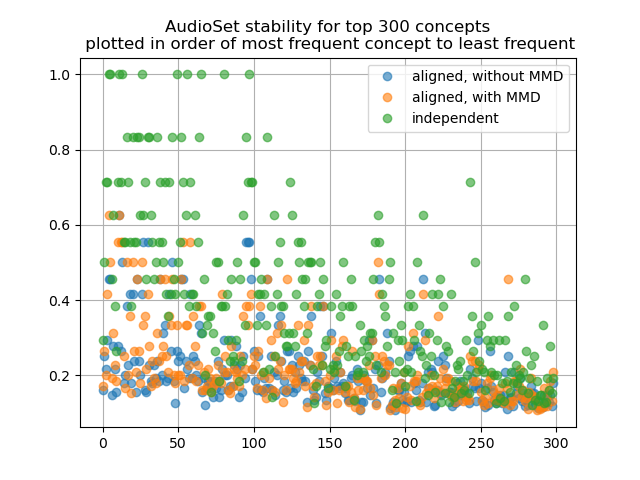
\includegraphics[width=0.45\textwidth]{images/results/audioset_stability.png}
    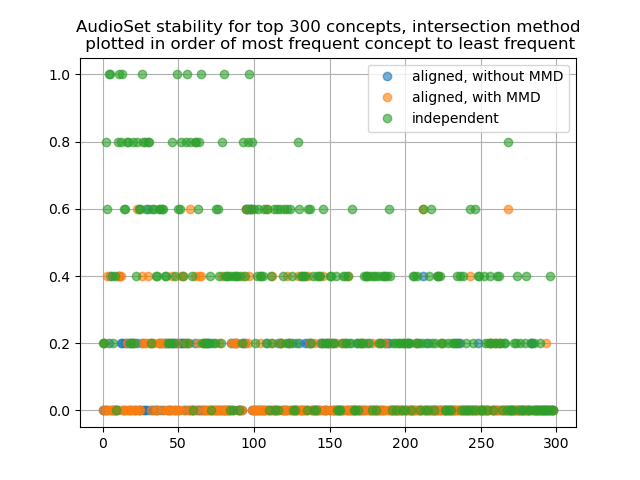
\includegraphics[width=0.45\textwidth]{images/results/audioset_stability_ixn.png}
    \caption{
        Stability of model variants for AudioSet. y-axis is relative frequency of concepts (most frequent = 0)
    }
\end{figure}


\begin{figure}[H]
    \centering
    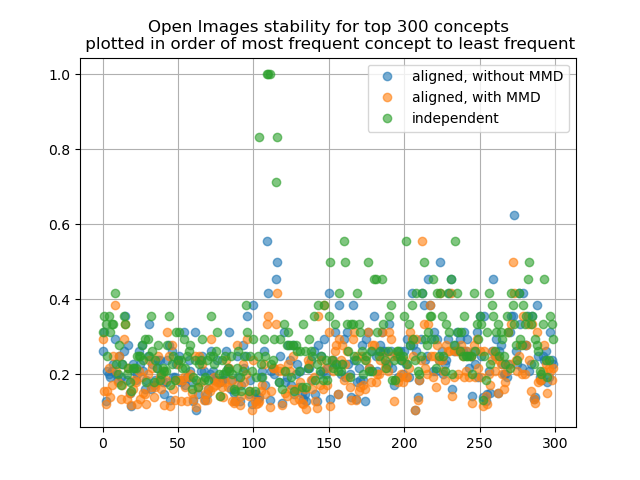
\includegraphics[width=0.45\textwidth]{images/results/openimages_stability.png}
    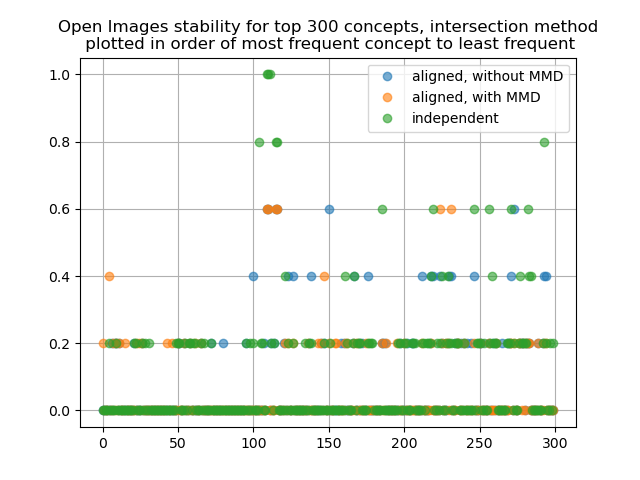
\includegraphics[width=0.45\textwidth]{images/results/openimages_stability_ixn.png}
    \caption{
        Stability of model variants for Open Images. y-axis is relative frequency of concepts (most frequent = 0)
    }
\end{figure}

\subsection{Other findings}
\subsubsection{The role of MMD}

Using MMD as a loss function has the effect of forcing $f(x)$ and $y$ to have the same distribution, and  $g(y)$ and $x$ to have the same distribution. Therefore it is reasonable that it should have a positive effect on alignment accuracy. However if the weighting of the MMD loss is high relative to glove loss, there is more pressure for distribution  matching but less pressure for good embeddings which can result in dysfunctional embeddings where all the concepts in the intersection are clustered together as shown in Figure \ref{fig:dysfunctional_clusters}. 

\subsubsection{Entropies and variances}

The entropies no longer correlate negatively with frequency of concepts, in the aligned embeddings. It is more appropriate to say they are now close to independent of the frequency of concepts, since the correlation is near zero. 

\subsubsection{GloVe loss scaling}
If the GloVe loss was not scaled by the ratio of concepts (see Section \ref{section:gloveloss}), the effect of this was to cause the (intersecting) concepts in the embedding to exhibit poor semantic organization.



%\begin{itemize}
%    \item Alignment accuracies of greater than 95\% were achieved for both domains ($f(x) \rightarrow y$ and $g(y) \rightarrow x$). % This was contingent on taking 10 samples for each embedding in each batch. If only 1 sample per embedding was taken, only 90\% accuracy was achieved. This is probably because using 10 samples acts like data augmentation. 
%\end{itemize}

\chapter{Further discussion and conclusions}

\todo[inline]{Brief summary of everything so far, suggestions for future work. }

\section{Summary of results}

\subsection{Restatement of project aims}

\begin{itemize}
    \item Learn independent probabilistic embeddings (represented by multidimensional Gaussian distributions with diagonal covariance matrix) for concepts in the Open Images and AudioSet domains.
    \item Investigate the quality of these embeddings and whether any insights can be gained from the variances.
    \item Learn jointly aligned probabilistic embeddings for concepts in the Open Images and AudioSet domains, in a semi-supervised way (marking the known correspondences between datasets). 
    \item Investigate the quality of the aligned embeddings compared to the independently learned embeddings. 
\end{itemize}

\subsection{Probabilistic embeddings}

\begin{itemize}
    \item The variances of the probabilistic embeddings, when expressed as entropies,  correlate negatively with co-occurrence frequency. Concepts which occur less frequently in the input data have a higher variance. 
    \item The means of the probabilistic embeddings represent sensible clusters when viewed through t-SNE dimensionality reduction. 
    \item Qualitatively, items in the concept hierarchy that represent very abstract concepts from the point of view of the hierarchy (``Cat", ``Dog") have nearest neighbours that are not very well clustered (show example). Items that are more specific (``Domestic short-haired cat")  have nearest neighbours that are more sensible (also show example). 
\end{itemize}

\subsection{Semi-supervised learning of aligned embeddings}

\begin{itemize}
    \item Our algorithm successfully learned jointly aligned embeddings from two modalities, OpenImages containing 19996 concepts and AudioSet containing 526 concepts, with an intersection of 230 concepts. No post-processing of the learned embeddings was necessary for alignment. 
    \item The 230 intersecting concepts were used as semi-supervised input into the algorithm; 230 concept instances were known to correspond.
    \item Alignment accuracy of more than 95\% was obtained between the two domains, for the intersecting concepts.
    \item However convergence to this level of accuracy while still maintaining sensible clustering (avoiding the degenerate case displayed in figure \ref{fig:dysfunctional_cluster} required the following:
    \begin{itemize}
        \item 10 samples per embedding in the mini-batch be used in each training step. This probably acts like data augmentation. 
        \item GloVe loss to be scaled by the ratio of concepts; since Open Images had 19996 concepts and AudioSet 526, GloVe loss for Open Images was multiplied by 19996 / 526. The cause of this requirement has not been investigated. 
        \item The criterion for saving the embeddings was when the mean alignment accuracy (of both OpenImages and AudioSet embeddings) was the lowest. Knowing that the independently learned probabilistic embeddings for AudioSet required more epochs of training to converge than the similar case of Open Images, it is possible that the point of greatest alignment accuracy for AudioSet is at a different epoch than for Open Images. 
    \end{itemize}
    \item The usage of the empirical MMD statistic as a loss function increased alignment accuracy for both domains.
    \item Embedding quality as measured by Spearman correlation of embedding pair similarity and WordNet similarity was greater for the aligned Open Images embeddings than the independently learned Open Images embeddings.
    \item Embedding quality by the same metric was decreased for the aligned AudioSet embeddings compared to the independently learned AudioSet embeddings. 
    \item The MMD statistic increased embedding quality as measured by the Spearman correlation metric for both Open Images and AudioSet domains, compared to the case of not using the MMD statistic. 
    \item There was less correlation between the entropy of the learned embeddings compared to the frequency of the occurrence of each concept, for aligned embeddings, compared to independently learned embeddings. (Could we expect that the variance of the distributions is less meaningful?)
\end{itemize}

\subsection{Computational performance}
\begin{itemize}
    \item Runtime - 150 epochs takes half an hour with saving models at lowest rate, convergence was fairly fast
    \item Scalability - would it scale to more concepts - the bottleneck part of the process is actually creating the co-occurrence matrix. 
\end{itemize}

\section{Further directions}

\begin{itemize}
    \item Reduce the proportion of concept intersections used from 230 to 0 gradually?
    \item Investigate if the highly imbalanced dataset (19996 concepts in Open Images vs 526 in AudioSet) causes other issues; already came across one, which was that the GloVe loss needed to be scaled to achieve good convergence. 
    \item The highly non-overlapping concept sets mean that there are many concepts present in Open Images that are not exactly present in AudioSet.
    \item However, the Open Images concepts are actually at many levels of hierarchy. For example there are many different types of cat (Malayan cat, Tabby cat, Siamese cat) and many different types of bread. Thus many of these may actually map to a single concept in AudioSet. 
    \item Use hierarchical embeddings (Poincare embeddings for example). It is clear that there are clusters of concepts, and preserving the structure between these clusters is desirable. For example, there are many different types and hierarchies of cats and dogs represented in the Open Images dataset, but only a few concepts in this hierarchy in AudioSet. The obvious modification to make would be to align the parent concepts for example ``Cat" and ``Dog" as a first pass, and then to attempt to align the subclasses around those anchor concepts. 
    \item An obvious limitation of using Open Images and AudioSet is that there are many aural concepts that do not have a visual representation. 
    \item Better results may perhaps be obtained by trying to align embeddings derived from Open Images and text, but then we would have to resolve the following technical problems
    \begin{itemize}
        \item How to resolve words to the Open Images namespace; one such possibility was used when running similarity comparisons with WordNet, described in the previous chapter. 
        \item How to extract not just single words but phrases from the text, for example ``domestic short-haired cat"
    \end{itemize}
\end{itemize}

\subsection{Unsupervised learning of aligned embeddings}
\begin{itemize}
    \item To truly mimic human learning, the ultimate aim is to learn aligned embeddings in a completely unsupervised fashion. 
    \item In this situation, the concept universes for both domains are known, as are the items in the intersection.
    \item However the specific embeddings in the intersection in each domain would not be directly mapped in the losses during learning. Aggregate statistics of the domain intersection might be used, such as the MMD.
    \item Preliminary work was unable to produce accuracies greater than 1\% for totally unsupervised alignment, using the same configuration as the semi-supervised case, only excluding the distance loss that related $||f(x) - y||$ and $||g(y) - x||$, even when run to high numbers of epochs. 
    \item MMD and other distribution similarity measures from \cite{torchtwosample} were tried.
    \item Further preliminary work also tested the Manifold Alignment GAN (\cite{magan}) and the Wasserstein GAN (\cite{WassersteinGAN}). Neither of these produced any feasible alignment. Mode collapse (all concepts mapping to the same embedding) was at first an issue, but even after using the minibatch discrimination technique \todo[inline]{CITE}, no feasible alignment was found. 
    \item Since GANs do well on problems where the input data fall into specific discernible classes, and our dataset does not have this characteristic (though there are discernible classes, they are indistinct as befits a human taxonomy of concepts rather than visual representations of 10 digits, or works by different artists), it is reasonable that a naive GAN might not work. 
    

\end{itemize}

%\chapter{Stuff that doesn't belong anywhere at the moment}



\section{Probabilistic embeddings learnt independently}

\begin{itemize}
    \item Each modality (images and audio) was learnt from separate co-occurrence data
    \item Means of the embeddings were examined 
    \begin{itemize}
        \item Similarity matrix calculated for means using dot product
        \item Because dot product is used in the Glove loss
        \item Then self-correlation between similarity matrix for means is calculated
        \item To see if there is a structure between seeds - if there is, we expect the self-correlation matrices to look the same between seeds.
        \item TSNE plots for different seeds to show clustering works fine
        \item Make figure showing different clusters eg. sports, cats, dogs, and different relationships for different random seeds (stochasticity in learnt embeddings). 
        \item TSNE seed was set to the same value and that causes the same plot if the input data is the same, therefore if plots are not the same, input data is not the same. 
    \end{itemize}
    \item Variances were converted to entropy and examined
    \begin{itemize}
        \item Entropies have the same distribution over all seeds (figure)
        \item Entropies are correlated with frequency: higher entropy (higher variance) corresponds to lower frequency words. (show spearman correlation)
    \end{itemize}
\end{itemize}


\section{Assorted bits from experimental method}
\begin{itemize}
    \item Semi-supervised alignment: 
    \begin{itemize}
        \item Openimages dataset with 19996 concepts (x), AudioSet has 526 concepts (y)
        \item Intersection of 230
        \item We have co-occurrence data for both datasets
        \item We will learn 2 sets of embeddings simultaneously, having an aligner network for each
        that learns $f(x) \approx y$ and $g(y) \approx x$
        \item Initial idea- Loss comprises the following items:
        \begin{itemize}
            \item Glove loss for x and y over all concepts
            \item Cycle loss for x: $f(g(y)) - x$ and y: $g(f(x)) - y$ over all concepts
            \item Supervised loss for x: $f(x) - y$ and y: $g(y) - x$ for the intersection of concepts
        \end{itemize}
        \item We learn both deterministic and probabilistic embeddings \todo[inline]{Not sure what to do with the deterministic ones}
        \item For probabilistic embeddings we use an optional additional loss item: Maximum mean discrepancy loss \cite{MMDGretton}, between f(x) with y and g(y) with x,  which provides additional ``pressure" needed to force the distributions to be the same. 
        \begin{itemize}
            \item MMD with a characteristic kernel will be 0 if the distributions are the same and certain conditions are met of the embedding space. 
            \item Use a Gaussian kernel which is characteristic.
            \item MMD is like infinite moment matching, if a characteristic kernel is used. 
        \end{itemize} 
    \end{itemize}
    \item Convergence is measured by accuracy, which is how well the known mapped concepts map to each other.
    \item For example, if we take $x$ to be the embedding of ``Cat"  in Openimages, and $f(x)$ to be the mapping of Openimages to AudioSet, then we expect that the nearest neighbour of $f(x)$ should be the embedding of ``Cat" in AudioSet. 
    \item Use mismatch loss for x: fraction of f(x) whose nearest neighbour is not the corresponding known y, and mismatch loss for y vice versa
    \item Analysis of results of how the unsupervised concepts (for example the ~19500 concepts that exist in Openimages that don't exist in AudioSet) form structure
\end{itemize}


\begin{itemize}
    \item Unsupervised alignment
    \begin{itemize}
        \item There does not appear to be a single distance metric that works. 
        \item Using multiple distance metrics just results in divergence which makes sense, because it complicates the loss function surface making the minimum harder to find. 
        \item Tried 3 GANs and none of them worked: Normal GAN, MAGAN, Wasserstein GAN
    \end{itemize}
    \item If writing up why it didn't work:
    \begin{itemize}
        \item What was tried and why it was plausible
        \item How to conclude it didn't work
        \item Any possible reasons for why
    \end{itemize}
\end{itemize}

\section{Alignment}

    \begin{itemize}
        \item In its simplest form: Learning how to map between 2 vector spaces. Dataset will often have large dimensionality. Compress datasets into a lower-dimensional representation while retaining semantic / structural similarity. 
        \item Second order isomorphism - \cite{SHEPARD19701} - functional relationships between concept clusters. 
        \begin{itemize}
            \item Therefore if there is a ``real-world" connection between some concepts - as evidenced by co-occurrence statistics from different modalities - we should observe the same connection between representations of those concepts, in our case, embeddings. 
            \item \cite{GOLDSTONE2002295}: The meaning of a concept is highly tied in with its relationships to other concepts within that modality. Similarity relationships between concepts within the same system can therefore be used to translate, or map, between systems. 
            \item \cite{GOLDSTONE2002295}: Cannot learn concepts singularly; can only understand once an entire system of related concepts has been learnt. \cite{GOLDSTONE2002295} suggests that the conceptual web can be augmented with systems of externally grounded meaning to come up with a system that is better than that using only one. 
            \item https://www.jstor.org/stable/2108085 - ``translation holism" - systems can only be translated if both systems contain enough similar concepts. If the meaning of a concept depends on that concept's place in the system, and the systems are different, then the meanings in the two systems will be different. 
            \item \cite{GOLDSTONE2002295} ABSURDIST was an early attempt to find ``correspondence" (their term for alignment) across two systems of concepts. ABSURDIST does not require a one to one mapping between concepts in systems and two concepts correspond if they have equivalent roles in their respective systems.
            \item ABSURDIST finds concepts that correspond between systems but it does not map these to any external world representation. It also does not attempt to include any hierarchical information, like that a dog is a type of animal. No specific relationships between concepts like is-a, has-a, part-of, used-for, or causality, are captured. 
            \item However ABSURDIST takes as its only inputs similarity matrices that some external agent (a German-English bilingual human, in the paper's example) has created. 
            \item ABSURDIST attempts to show that the relationships between parts of a system provide enough information necessary for an observer to translate between two such systems- this is the main point of interest in ABSURDIST. 
            \item There are no constraints on what the two systems are, or even on the number of concepts present in each system, in order for correspondences to exist. This is analogous to our problem; the two systems represent the modalities (images and audio), and the number of concepts  is quite unbalanced. 
            \item ABSURDIST found that while within-system relationships are enough to find a translation, this translation can be made more robust to noise by adding external, extrinsic information on correspondences (certain correspondences are weighted with higher values). 
        \end{itemize}
    \end{itemize}
    
    
    
\section{Raw data for Spearman correlations with human similarity datasets}
    
    

\subsubsection{Comparison with MTURK-771}

\todo[inline]{Condense all tables into one}


Only Open Images was compared with this dataset, as there were too few pairs overlapping with AudioSet (only three). 

\subsubsection{Open Images, Spearman correlation with MTURK-771 similarity}\\

\begin{tabular}{lrrrrr}
\toprule
{} &  independent &   aligned &  aligned\_acc &  aligned\_mmd &  aligned\_mmd\_acc \\
\midrule
1    &     0.357040 &  0.305814 &     0.947826 &     0.331085 &         0.947826 \\
2    &     0.342876 &  0.271306 &     0.956522 &     0.296354 &         0.982609 \\
3    &     0.375564 &  0.338173 &     0.934783 &     0.287192 &         0.956522 \\
4    &     0.342911 &  0.299614 &     0.952174 &     0.289880 &         0.965217 \\
5    &     0.357850 &  0.255958 &     0.947826 &     0.225208 &         0.960870 \\
6    &     0.373989 &  0.308962 &     0.952174 &     0.271217 &         0.973913 \\
7    &     0.347433 &  0.296559 &     0.965217 &     0.292202 &         0.965217 \\
8    &     0.343246 &  0.284002 &     0.969565 &     0.283377 &         0.952174 \\
9    &     0.340476 &  0.279059 &     0.956522 &     0.271877 &         0.956522 \\
10   &     0.366640 &  0.267160 &     0.960870 &     0.283802 &         0.952174 \\
\midrule
mean &     0.354803 &  0.290661 &     0.954348 &     0.283219 &         0.961304 \\
\bottomrule
\end{tabular}\\


\subsubsection{Open Images, differences of Spearman correlation between aligned model variant and MTURK-771 and independent embeddings}

\begin{tabular}{lrr}
\toprule
{} &   aligned &  aligned\_mmd \\
\midrule
1    & -0.051227 &    -0.025955 \\
2    & -0.071571 &    -0.046522 \\
3    & -0.037390 &    -0.088372 \\
4    & -0.043297 &    -0.053031 \\
5    & -0.101893 &    -0.132642 \\
6    & -0.065027 &    -0.102772 \\
7    & -0.050874 &    -0.055231 \\
8    & -0.059244 &    -0.059869 \\
9    & -0.061417 &    -0.068599 \\
10   & -0.099481 &    -0.082839 \\
\midrule
mean & -0.064142 &    -0.071583 \\
\bottomrule
\end{tabular}\\



\subsection{Comparison with WordNet}

\subsubsection{Open Images, Spearman correlation with WordNet similarity}

\begin{tabular}{lrrrrr}
\toprule
{} &  independent &   aligned &  aligned\_acc &  aligned\_mmd &  aligned\_mmd\_acc \\
\midrule
1    &     0.204645 &  0.229008 &     0.947826 &     0.228036 &         0.947826 \\
2    &     0.195614 &  0.221148 &     0.956522 &     0.230173 &         0.982609 \\
3    &     0.199725 &  0.239952 &     0.934783 &     0.239973 &         0.956522 \\
4    &     0.210023 &  0.233182 &     0.952174 &     0.228500 &         0.965217 \\
5    &     0.190570 &  0.225954 &     0.947826 &     0.226141 &         0.960870 \\
6    &     0.206630 &  0.238630 &     0.952174 &     0.236737 &         0.973913 \\
7    &     0.207851 &  0.229461 &     0.965217 &     0.238660 &         0.965217 \\
8    &     0.215203 &  0.217090 &     0.969565 &     0.218335 &         0.952174 \\
9    &     0.216922 &  0.223884 &     0.956522 &     0.233538 &         0.956522 \\
10   &     0.206950 &  0.225371 &     0.960870 &     0.230410 &         0.952174 \\
\midrule
mean &     0.205413 &  0.228368 &     0.954348 &     0.231050 &         0.961304 \\
\bottomrule
\end{tabular}

\subsubsection{Open Images, differences of Spearman correlation between aligned model variant and WordNet and independent embeddings} \\

\begin{tabular}{lrr}
\toprule
{} &   aligned &  aligned\_mmd \\
\midrule
1    &  0.024363 &     0.023391 \\
2    &  0.025535 &     0.034559 \\
3    &  0.040227 &     0.040248 \\
4    &  0.023160 &     0.018477 \\
5    &  0.035384 &     0.035571 \\
6    &  0.032000 &     0.030108 \\
7    &  0.021610 &     0.030809 \\
8    &  0.001887 &     0.003131 \\
9    &  0.006962 &     0.016616 \\
10   &  0.018421 &     0.023459 \\
\midrule
mean &  0.022955 &     0.025637 \\
\bottomrule
\end{tabular}


\subsubsection{AudioSet, Spearman correlation with WordNet similarity}

\begin{tabular}{lrrrrr}
\toprule
{} &  independent &   aligned &  aligned\_acc &  aligned\_mmd &  aligned\_mmd\_acc \\
\midrule
1    &     0.138980 &  0.162728 &     0.947826 &     0.152753 &         0.965217 \\
2    &     0.132803 &  0.130027 &     0.969565 &     0.147193 &         0.982609 \\
3    &     0.157127 &  0.174757 &     0.956522 &     0.133395 &         0.978261 \\
4    &     0.146678 &  0.148297 &     0.956522 &     0.168750 &         0.956522 \\
5    &     0.116176 &  0.151164 &     0.943478 &     0.152322 &         0.969565 \\
6    &     0.144309 &  0.134435 &     0.973913 &     0.125409 &         0.969565 \\
7    &     0.149543 &  0.133959 &     0.947826 &     0.169722 &         0.973913 \\
8    &     0.140360 &  0.182683 &     0.960870 &     0.127695 &         0.952174 \\
9    &     0.147353 &  0.135669 &     0.960870 &     0.187408 &         0.978261 \\
10   &     0.149795 &  0.165782 &     0.965217 &     0.142835 &         0.978261 \\
\midrule
mean &     0.142313 &  0.151950 &     0.958261 &     0.150748 &         0.970435 \\
\bottomrule
\end{tabular}


\subsubsection{AudioSet, differences of Spearman correlation between aligned model variant and WordNet and independent embeddings with WordNet}

\begin{tabular}{lrr}
\toprule
{} &   aligned &  aligned\_mmd \\
\midrule
1    &  0.023748 &     0.013773 \\
2    & -0.002776 &     0.014390 \\
3    &  0.017631 &    -0.023732 \\
4    &  0.001618 &     0.022072 \\
5    &  0.034988 &     0.036146 \\
6    & -0.009875 &    -0.018901 \\
7    & -0.015584 &     0.020179 \\
8    &  0.042323 &    -0.012665 \\
9    & -0.011684 &     0.040055 \\
10   &  0.015986 &    -0.006961 \\
\midrule
mean &  0.009637 &     0.008436 \\
\bottomrule
\end{tabular}

\subsection{Comparison with ILSVRC}

\subsubsection{Open Images, Spearman correlation with ILSVRC similarity}

\begin{tabular}{lrrrrr}
\toprule
{} &  independent &   aligned &  aligned\_acc &  aligned\_mmd &  aligned\_mmd\_acc \\
\midrule
1    &     0.523743 &  0.493222 &     0.947826 &     0.488418 &         0.947826 \\
2    &     0.470860 &  0.460144 &     0.956522 &     0.457864 &         0.982609 \\
3    &     0.482953 &  0.486438 &     0.934783 &     0.433406 &         0.956522 \\
4    &     0.514398 &  0.531787 &     0.952174 &     0.482189 &         0.965217 \\
5    &     0.504501 &  0.465994 &     0.947826 &     0.456137 &         0.960870 \\
6    &     0.541152 &  0.472602 &     0.952174 &     0.450753 &         0.973913 \\
7    &     0.506350 &  0.468013 &     0.965217 &     0.446900 &         0.965217 \\
8    &     0.553240 &  0.458478 &     0.969565 &     0.468173 &         0.952174 \\
9    &     0.507937 &  0.463128 &     0.956522 &     0.438866 &         0.956522 \\
10   &     0.531030 &  0.463582 &     0.960870 &     0.451747 &         0.952174 \\
\midrule
mean &     0.513617 &  0.476339 &     0.954348 &     0.457445 &         0.961304 \\
\bottomrule
\end{tabular}

\subsubsection{Open Images, differences of Spearman correlation between aligned model variant and ILSVRC and independent embeddings} \\

\begin{tabular}{lrr}
\toprule
{} &   aligned &  aligned\_mmd \\
\midrule
1    & -0.030521 &    -0.035326 \\
2    & -0.010716 &    -0.012996 \\
3    &  0.003485 &    -0.049548 \\
4    &  0.017389 &    -0.032209 \\
5    & -0.038507 &    -0.048364 \\
6    & -0.068550 &    -0.090399 \\
7    & -0.038337 &    -0.059450 \\
8    & -0.094763 &    -0.085067 \\
9    & -0.044809 &    -0.069071 \\
10   & -0.067448 &    -0.079283 \\
\midrule
mean & -0.037278 &    -0.056171 \\
\bottomrule
\end{tabular}

\subsubsection{AudioSet, Spearman correlation with ILSVRC similarity}

\begin{tabular}{lrrrrr}
\toprule
{} &  independent &   aligned &  aligned\_acc &  aligned\_mmd &  aligned\_mmd\_acc \\
\midrule
1    &     0.634553 &  0.683402 &     0.947826 &     0.502208 &         0.965217 \\
2    &     0.584539 &  0.686640 &     0.969565 &     0.650786 &         0.982609 \\
3    &     0.646683 &  0.427680 &     0.956522 &     0.617364 &         0.978261 \\
4    &     0.560294 &  0.609964 &     0.956522 &     0.648891 &         0.956522 \\
5    &     0.562203 &  0.513384 &     0.943478 &     0.578213 &         0.969565 \\
6    &     0.630897 &  0.609099 &     0.973913 &     0.503820 &         0.969565 \\
7    &     0.539494 &  0.563158 &     0.947826 &     0.546268 &         0.973913 \\
8    &     0.552983 &  0.674972 &     0.960870 &     0.681851 &         0.952174 \\
9    &     0.523634 &  0.718003 &     0.960870 &     0.680956 &         0.978261 \\
10   &     0.607010 &  0.717317 &     0.965217 &     0.698815 &         0.978261 \\
\midrule
mean &     0.584229 &  0.620362 &     0.958261 &     0.610917 &         0.970435 \\
\bottomrule
\end{tabular}


\subsubsection{AudioSet, differences of Spearman correlation between aligned model variant and ILSVRC and independent embeddings with ILSVRC}


\begin{tabular}{lrr}
\toprule
{} &   aligned &  aligned\_mmd \\
\midrule
1    &  0.048850 &    -0.132345 \\
2    &  0.102101 &     0.066247 \\
3    & -0.219003 &    -0.029319 \\
4    &  0.049670 &     0.088598 \\
5    & -0.048820 &     0.016010 \\
6    & -0.021799 &    -0.127078 \\
7    &  0.023664 &     0.006774 \\
8    &  0.121990 &     0.128868 \\
9    &  0.194369 &     0.157321 \\
10   &  0.110307 &     0.091806 \\
\midrule
mean &  0.036133 &     0.026688 \\
\bottomrule
\end{tabular}
    
\section{Measures of statistical distance}

\subsubsection{Energy distance}

Energy statistics, as described in \cite{energystatistics}, are measures of distance between statistical observations. They are based on the idea of gravitational potential energy as a function of the distance between two objects. The analogy is that the statistical observations are like large bodies which have a statistical potential energy depending on the statistical distance between them. 

[More on reasoning on why energy statistics are useful from \cite{energystatistics}]

The generic energy statistic for a random sample $\vecx_1, ..., \vecx_n$ and kernel function $k$, where $k$ is a symmetric function of Euclidean distances between the samples, has the following expression:

\begin{equation}
\label{eq:energystatistic}
\begin{split}
U_n = \frac{1}{n(n-1)} \sumin \sum_{j \neq i}^n k(\vecx_i, \vecx_j)
\end{split}
\end{equation}

We can see that this looks similar to the MMD expression in (\ref{eq:mmd}). If the MMD is used with a Gaussian kernel, then the MMD is a sum of energy statistics.

The energy statistic used to test for equal distributions as described in \cite{energystatistics} takes the following form. In the below,

\begin{itemize}
    \item $\vecx_i$ are $m$ samples from one distribution  $X$
    \item $\vecy_j$ are $n$ samples from the other distribution $Y$
\end{itemize}

\begin{equation}
\label{eq:energydistance}
\begin{split}
E(X, Y) &= \frac{2}{nm} \sumim \sumjn |\vecx_i - \vecy_j| - \frac{1}{n^2} \sumin \sumjn | \vecx_i - \vec_j| \\
&- \frac{1}{m^2} \sumim \sumjm |\vecy_i - \vecy_j|
\end{split}
\end{equation}

As with MMD, the implementation in the \texttt{torch-two-sample / https://torch-two-sample.readthedocs.io} library \cite{torchtwosample} was used. 

The energy statistic, when used in the loss function even with scaling (multiplying by a large factor), only achieved up to 50\% convergence of alignment. 

\subsubsection{Smoothed graph statistics}
\cite{torchtwosample} describes the problem of learning rich implicit models, from which we can get samples, but not evaluate their density. The embedding alignment problem can be considered in this class; we have samples from the distributions $f(x)$, $g(y)$, $x$ and $y$ but we do not have access to the probability densities of these models. \cite{torchtwosample} describes that a two-sample distributional test for distributional identity should be a good loss function for learning such an implicit model, as if the loss can decrease to zero, the distributions should be identical. 

However, some of these two-sample tests are not differentiable, and so cannot be used as loss functions in backpropagation frameworks. The authors of \cite{torchtwosample} have implemented smoothed, and therefore differentiable, versions of two such tests, the Friedman-Rafsky and k-nearest-neighbour graph tests. This theory is briefly summarised here and we refer readers to the original paper for much more detail. 

We introduce the following notation, which differs from that in \cite{torchtwosample} to avoid overloading previously defined terms in this document. 

\begin{itemize}
    \item $P$ is the distribution from which the points $X = \{\vecx_1, ..., \vecx_n \}$ are drawn.
    \item $Q$ is the distribution from which the points $Y = \{\vecy_1, ..., \vecy_n \}$ are drawn.
    \item $H(X) = (X, E)$ is the directed graph defined over the vertex set $X = \{\vecx_1, ..., \vecx_n \}$, with edges $E$.
    \item $J(Y) = (Y, F) $ is the directed graph defined over the vertex set $Y = \{\vecy_1, ..., \vecy_m \}$, with edges $F$. 
    \item These graphs are weighted with the distance function $d(\vecx, \vecx') = || \vecx - \vecx'||$, and we will denote with $d(e)$ the weight of the edge $e$ using distance function $d$. 
    \item For a labelling of vertices $\pi: X \rightarrow \{1, 2\}$ and any edge $e$ whose vertices $i$ and $j$ are adjacent, define $\Delta_{\pi}(e)$ to be 1 if $e$'s end points have different labels under the mapping $\pi$. 
\end{itemize}

The generic framework for the graph tests follows these steps:

\begin{enumerate}
    \item Let $Z$ be the union of the samples $X$ and $Y$ and let $K(Z)$ be the graph defined over all points. Define a mapping $\pi^* : Z \rightarrow \{1, 2\}$ such that $\pi^*(X) = 1$ and $\pi^*(Y) = 2$.
    \item Use an algorithm $A$ to choose a subset $U^* = A(K(Z))$ of the edges of $Z$, the idea being that this algorithm should encode some sort of neighbourhood structure.
    \begin{itemize}
        \item The Friedman-Rafsky test (CITE) uses the minimum spanning tree of $H(X)$ as the algorithm for selecting the neighbourhood structure $U^*$. 

        \item The k-nearest neighbours test adds an edge $e$ to $U^*$ if the starting point is one of the k nearest neighbours of the end point under the distance measure $d$.
    \end{itemize}
    \item The statistic $T_{\pi^*}(U^*) = \sum_{e \in U^*} \Delta_{\pi^*} (e)$ defines how many edges in $U^*$ join points from $X$ and $Y$. 
    \item If $T_{\pi^*}$ is high, then many edges join points from $X$ and $Y$, and $X$ and $Y$ are highly aligned. When using this statistic as a loss function, the negative of this must be minimised.
\end{enumerate}


In order to use $T_{\pi^*}$ in a loss function with backpropagation, we need to be able to calculate the derivatives $\frac{\partial T}{\partial \vecx_i}$ which normally do not exist. In \cite{torchtwosample} the strategy cited is to smooth these functions to make them continuously differentiable by turning them into expectations of probabilistic models in the exponential family. 


We can express the optimal neighbourhood mapping $U^*$ as 

\begin{equation}
\begin{split}
U^* &= \argmin{U \subseteq E} \sum_{e \in U} d(e) \spaced{such that} v(U) = 1 \\
&\spaced{and further define} \vecd \spaced{to be the vector of edge weights} d(e). 
\end{split}
\end{equation}

where $v: 2^{|E|} \rightarrow \{0, 1 \}$ is a mapping indicating if the set of edges is valid under the constraints of algorithm $A$, for example if each vertex has $k$ neighbours for the KNN test, or if the set of edges forms a valid set of minimum spanning trees in the Friedman-Rafsky test case. 

The aim is to find a probability distribution over $U$ whose expectation can be used in place of $T_{\pi^*}$. Without proof, we state the result from \cite{torchtwosample} that the following exponential family function suffices:

\begin{equation}
\label{eq:smoothed}
\begin{split}
P(U | \vecd / \lambda) &= \exp\Big[-\sum_{e \in U} d(e) / \lambda - A(-\vecd / \lambda \Big] v(U)
\end{split}
\end{equation}

where $\lambda$ is a hyperparameter (the ``temperature parameter") and $A(-\vecd / \lambda)$ is the log-partition function  that normalises the distribution. $U^*$ is thus a maximum a posteriori configuration for $P(U | \vecd/\lambda)$, and as $\lambda$ tends to 0,  $P(U | \vecd/\lambda)$ will tend to the MAP estimate. 

If we use the expectation $E_{U}[T_{\pi^*}(U)]$ in place of the original statistic $T_{\pi^*(U^*)}$, since $P(U)$ (\ref{eq:smoothed}) is a member of the exponential family, we can compute its first and second moments, which lead to the values of the smoothed statistic as well as its derivative.  [Add more details]

The PyTorch implementations in the \texttt{torch-two-sample} library  were used. The following were observed:

\begin{itemize}
    \item For $\lambda$ hyperparameter values of 0.01, the smoothed FR statistic converged to accuracy of about 60\%. 
    \item For hyperparameter values of 0.1, 1, and 5, the smoothed FR statistic simply diverged with increasing numbers of epochs and accuracy was at most 2\%.  , 
    \item For $\lambda$ hyperparameter values of 0.01, 0.1, 1, and 5, smoothed 1-NN was used. The KNN statistic decreased but accuracy never went above 2\%.
\end{itemize}

%It is surprising that these graph-based losses did not work at all in terms of aligning the embeddings using the intersection of concepts. The hypothesis was that loss functions based on graph structure should prove useful in picking out second-order isomorphisms as previously stated. 

    
\section{Results}
\begin{itemize}
    \item Convergence means asymptotically small glove loss, cycle loss, supervised loss
    \item Also accuracy of alignment higher than 97\%
    \item Had to be scaled- MMD loss multiplied by factor 1, caused convergence to 50\% alignment and then divergence down to 0.
    \item Multiplied by 10 had the same behaviour, convergence to 60\% alignment then divergence
    \item As the objective of this experiment is to achieve alignment, the partially-aligned situations were not investigated. This could be a possibility for further investigation, perhaps in terms of mixing with another metric to see if this improved convergence. 
    \item Scaled MMD converged fast to within 30 epochs, but we ran to 50 epochs anyway
    \item However, 
    \item Therefore regularisation was applied to reduce the weights of the aligner MLP 
    \item As the regularisation parameter is increased, TSNE plots of the intersection of concepts + top 200, show that the points get "mixed" more and more. 
    \item Second set of experiments run with MMD = 100, 100 epochs and regularisations. Observed that the maximum mean accuracy (of both x and y) was some time before 100 epochs, and then it started to decrease again, so the embeddings were saved if the mean accuracy was greater than that averaged over the previous epoch. This was not necessary for the MMD 500 case because in the MMD 500 case, it decreased to the asymptote. 
\end{itemize}

\appendix

%\chapter{Appendix}
\chapter{}

\section{Graph-based measures of statistical distance}
\label{appendix:graphbased}
We introduce the following notation, which differs from that in \cite{torchtwosample} to avoid overloading previously defined terms in this document. 

\begin{itemize}
    \item $P$ is the distribution from which the points $X = \{\vecx_1, ..., \vecx_n \}$ are drawn.
    \item $Q$ is the distribution from which the points $Y = \{\vecy_1, ..., \vecy_n \}$ are drawn.
    \item $H(X) = (X, E)$ is the directed graph defined over the vertex set $X = \{\vecx_1, ..., \vecx_n \}$, with edges $E$.
    \item $J(Y) = (Y, F) $ is the directed graph defined over the vertex set $Y = \{\vecy_1, ..., \vecy_m \}$, with edges $F$. 
    \item These graphs are weighted with the distance function $d(\vecx, \vecx') = || \vecx - \vecx'||$, and we will denote with $d(e)$ the weight of the edge $e$ using distance function $d$. 
    \item For a labelling of vertices $\pi: X \rightarrow \{1, 2\}$ and any edge $e$ whose vertices $i$ and $j$ are adjacent, define $\Delta_{\pi}(e)$ to be 1 if $e$'s end points have different labels under the mapping $\pi$. 
\end{itemize}

The generic framework for the graph tests follows these steps:

\begin{enumerate}
    \item Let $Z$ be the union of the samples $X$ and $Y$ and let $K(Z)$ be the graph defined over all points. Define a mapping $\pi^* : Z \rightarrow \{1, 2\}$ such that $\pi^*(X) = 1$ and $\pi^*(Y) = 2$.
    \item Use an algorithm $A$ to choose a subset $U^* = A(K(Z))$ of the edges of $Z$, the idea being that this algorithm should encode some sort of neighbourhood structure.
    \begin{itemize}
        \item The Friedman-Rafsky test (CITE) uses the minimum spanning tree of $H(X)$ as the algorithm for selecting the neighbourhood structure $U^*$. 

        \item The k-nearest neighbours test adds an edge $e$ to $U^*$ if the starting point is one of the k nearest neighbours of the end point under the distance measure $d$.
    \end{itemize}
    \item The statistic $T_{\pi^*}(U^*) = \sum_{e \in U^*} \Delta_{\pi^*} (e)$ defines how many edges in $U^*$ join points from $X$ and $Y$. 
    \item If $T_{\pi^*}$ is high, then many edges join points from $X$ and $Y$, and $X$ and $Y$ are highly aligned. When using this statistic as a loss function, the negative of this must be minimised.
\end{enumerate}

In order to use $T_{\pi^*}$ in a loss function with backpropagation, we need to be able to calculate the derivatives $\frac{\partial T}{\partial \vecx_i}$ which normally do not exist. In \cite{torchtwosample} the strategy cited is to smooth these functions to make them continuously differentiable by turning them into expectations of probabilistic models in the exponential family. 

We can express the optimal neighbourhood mapping $U^*$ as 

\begin{equation}
\begin{split}
U^* &= \argmin{U \subseteq E} \sum_{e \in U} d(e) \spaced{such that} v(U) = 1 \\
&\spaced{and further define} \vecd \spaced{to be the vector of edge weights} d(e). 
\end{split}
\end{equation}

where $v: 2^{|E|} \rightarrow \{0, 1 \}$ is a mapping indicating if the set of edges is valid under the constraints of algorithm $A$, for example if each vertex has $k$ neighbours for the KNN test, or if the set of edges forms a valid set of minimum spanning trees in the Friedman-Rafsky test case. 

The aim is to find a probability distribution over $U$ whose expectation can be used in place of $T_{\pi^*}$. Without proof, we state the result from \cite{torchtwosample} that the following exponential family function suffices:

\begin{equation}
\label{eq:smoothed}
\begin{split}
P(U | \vecd / \lambda) &= \exp\Big[-\sum_{e \in U} d(e) / \lambda - A(-\vecd / \lambda \Big] v(U)
\end{split}
\end{equation}

where $\lambda$ is a hyperparameter (the ``temperature parameter") and $A(-\vecd / \lambda)$ is the log-partition function  that normalises the distribution. $U^*$ is thus a maximum a posteriori configuration for $P(U | \vecd/\lambda)$, and as $\lambda$ tends to 0,  $P(U | \vecd/\lambda)$ will tend to the MAP estimate. 

If we use the expectation $E_{U}[T_{\pi^*}(U)]$ in place of the original statistic $T_{\pi^*(U^*)}$, since $P(U)$ (\ref{eq:smoothed}) is a member of the exponential family, we can compute its first and second moments, which lead to the values of the smoothed statistic as well as its derivative. These functions can now be used as loss functions of which minimisation corresponds to the two inputs having greater graph similarity. 



%\bibliographystyle{apalike}
%\bibliography{refs}

\printbibliography

\end{document}